\documentclass[11pt]{article}%
\usepackage{geometry}%
\geometry{a4paper,
  lmargin=2cm,rmargin=2cm,tmargin=2.5cm,bmargin=2.5cm}

% \usepackage{array}
\usepackage{paralist}

\usepackage[svgnames, usenames, dvipsnames]{xcolor}
\xdefinecolor{RecColor}{named}{Aqua}
\xdefinecolor{IncColor}{named}{Aqua}
\xdefinecolor{ImpColor}{named}{PaleGreen}

% \usepackage{frcursive}

\usepackage{adjustbox}

%%%%%%%%%%%
\newcommand{\cRB}[1]{{\color{Red} \pmb{#1}}} %
\newcommand{\cR}[1]{{\color{Red} {#1}}} %
\newcommand{\cBB}[1]{{\color{Blue} \pmb{#1}}}
\newcommand{\cB}[1]{{\color{Blue} {#1}}}
\newcommand{\cGB}[1]{{\color{LimeGreen} \pmb{#1}}}
\newcommand{\cG}[1]{{\color{LimeGreen} {#1}}}

%%%%%%%%%%

\usepackage{diagbox} %
\usepackage{colortbl} %
\usepackage{multirow} %
\usepackage{pgf} %
\usepackage{environ} %
\usepackage{fancybox} %
\usepackage{textcomp} %
\usepackage{marvosym} %

%%%%%%%%%% pour qu'une cellcolor ne recouvre pas le trait du tableau
\usepackage{hhline}%

\usepackage{pgfplots}
\pgfplotsset{compat=1.10}
\usepgfplotslibrary{patchplots}
\usepgfplotslibrary{fillbetween}
\usepackage{tikz,tkz-tab}
\usepackage{ifthen}
\usepackage{calc}
\usetikzlibrary{calc,decorations.pathreplacing,arrows,positioning} 
\usetikzlibrary{fit,shapes,backgrounds}
\usepackage[nomessages]{fp}% http://ctan.org/pkg/fp

\usetikzlibrary{matrix,arrows,decorations.pathmorphing,
  decorations.pathreplacing} 

\newcommand{\myunit}{1 cm}
\tikzset{
    node style sp/.style={draw,circle,minimum size=\myunit},
    node style ge/.style={circle,minimum size=\myunit},
    arrow style mul/.style={draw,sloped,midway,fill=white},
    arrow style plus/.style={midway,sloped,fill=white},
}

%%%%%%%%%%%%%%
%%%%% écrire des inférieur égal ou supérieur égal avec typographie
%%%%% francaise
%%%%%%%%%%%%%

\renewcommand{\geq}{\geqslant}
\renewcommand{\leq}{\leqslant}
\renewcommand{\emptyset}{\varnothing}

\newcommand{\Leq}{\leqslant}
\newcommand{\Geq}{\geqslant}

%%%%%%%%%%%%%%
%%%%% Macro Celia
%%%%%%%%%%%%%

\newcommand{\ff}[2]{\left[#1, #2\right]} %
\newcommand{\fo}[2]{\left[#1, #2\right[} %
\newcommand{\of}[2]{\left]#1, #2\right]} %
\newcommand{\soo}[2]{\left]#1, #2\right[} %
\newcommand{\abs}[1]{\left|#1\right|} %
\newcommand{\Ent}[1]{\left\lfloor #1 \right\rfloor} %


%%%%%%%%%%%%%%
%%%%% tikz : comment dessiner un "oeil"
%%%%%%%%%%%%%

\newcommand{\eye}[4]% size, x, y, rotation
{ \draw[rotate around={#4:(#2,#3)}] (#2,#3) -- ++(-.5*55:#1) (#2,#3)
  -- ++(.5*55:#1); \draw (#2,#3) ++(#4+55:.75*#1) arc
  (#4+55:#4-55:.75*#1);
  % IRIS
  \draw[fill=gray] (#2,#3) ++(#4+55/3:.75*#1) arc
  (#4+180-55:#4+180+55:.28*#1);
  % PUPIL, a filled arc
  \draw[fill=black] (#2,#3) ++(#4+55/3:.75*#1) arc
  (#4+55/3:#4-55/3:.75*#1);%
}


%%%%%%%%%%
%% discontinuité fonction
\newcommand\pointg[2]{%
  \draw[color = red, very thick] (#1+0.15, #2-.04)--(#1, #2-.04)--(#1,
  #2+.04)--(#1+0.15, #2+.04);%
}%

\newcommand\pointd[2]{%
  \draw[color = red, very thick] (#1-0.15, #2+.04)--(#1, #2+.04)--(#1,
  #2-.04)--(#1-0.15, #2-.04);%
}%

%%%%%%%%%%
%%% 1 : position abscisse, 2 : position ordonnée, 3 : taille, 4 : couleur
%%%%%%%%%%
% \newcommand\pointG[4]{%
%   \draw[color = #4, very thick] (#1+#3, #2-(#3/3.75))--(#1,
%   #2-(#3/3.75))--(#1, #2+(#3/3.75))--(#1+#3, #2+(#3/3.75)) %
% }%

\newcommand\pointG[4]{%
  \draw[color = #4, very thick] ({#1+#3/3.75}, {#2-#3})--(#1,
  {#2-#3})--(#1, {#2+#3})--({#1+#3/3.75}, {#2+#3}) %
}%

\newcommand\pointD[4]{%
  \draw[color = #4, very thick] ({#1-#3/3.75}, {#2+#3})--(#1,
  {#2+#3})--(#1, {#2-#3})--({#1-#3/3.75}, {#2-#3}) %
}%

\newcommand\spointG[4]{%
  \draw[color = #4, very thick] ({#1+#3/1.75}, {#2-#3})--(#1,
  {#2-#3})--(#1, {#2+#3})--({#1+#3/1.75}, {#2+#3}) %
}%

\newcommand\spointD[4]{%
  \draw[color = #4, very thick] ({#1-#3/2}, {#2+#3})--(#1,
  {#2+#3})--(#1, {#2-#3})--({#1-#3/2}, {#2-#3}) %
}%

%%%%%%%%%%

\newcommand{\Pb}{\mathtt{P}}

%%%%%%%%%%%%%%%
%%% Pour citer un précédent item
%%%%%%%%%%%%%%%
\newcommand{\itbf}[1]{{\small \bf \textit{#1}}}


%%%%%%%%%%%%%%%
%%% Quelques couleurs
%%%%%%%%%%%%%%%

\xdefinecolor{cancelcolor}{named}{Red}
\xdefinecolor{intI}{named}{ProcessBlue}
\xdefinecolor{intJ}{named}{ForestGreen}

%%%%%%%%%%%%%%%
%%%%%%%%%%%%%%%
% barrer du texte
\usetikzlibrary{shapes.misc}

\makeatletter
% \definecolor{cancelcolor}{rgb}{0.127,0.372,0.987}
\newcommand{\tikz@bcancel}[1]{%
  \begin{tikzpicture}[baseline=(textbox.base), inner sep=0pt]
    \node[strike out, draw] (textbox) {#1}[thick, color=cancelcolor];
    \useasboundingbox (textbox);
  \end{tikzpicture}%
}
\newcommand{\bcancel}[1]{%
  \relax\ifmmode
    \mathchoice{\tikz@bcancel{$\displaystyle#1$}}
               {\tikz@bcancel{$\textstyle#1$}}
               {\tikz@bcancel{$\scriptstyle#1$}}
               {\tikz@bcancel{$\scriptscriptstyle#1$}}
  \else
    \tikz@bcancel{\strut#1}%
  \fi
}
\newcommand{\tikz@xcancel}[1]{%
  \begin{tikzpicture}[baseline=(textbox.base),inner sep=0pt]
  \node[cross out,draw] (textbox) {#1}[thick, color=cancelcolor];
  \useasboundingbox (textbox);
  \end{tikzpicture}%
}
\newcommand{\xcancel}[1]{%
  \relax\ifmmode
    \mathchoice{\tikz@xcancel{$\displaystyle#1$}}
               {\tikz@xcancel{$\textstyle#1$}}
               {\tikz@xcancel{$\scriptstyle#1$}}
               {\tikz@xcancel{$\scriptscriptstyle#1$}}
  \else
    \tikz@xcancel{\strut#1}%
  \fi
}
\makeatother

\newcommand{\xcancelRA}{\xcancel{\rule[-.15cm]{0cm}{.5cm} \Rightarrow
    \rule[-.15cm]{0cm}{.5cm}}}

%%%%%%%%%%%%%%%%%%%%%%%%%%%%%%%%%%%
%%%%%%%%%%%%%%%%%%%%%%%%%%%%%%%%%%%

\newcommand{\vide}{\multicolumn{1}{c}{}}

%%%%%%%%%%%%%%%%%%%%%%%%%%%%%%%%%%%
%%%%%%%%%%%%%%%%%%%%%%%%%%%%%%%%%%%


\usepackage{multicol}
% \usepackage[latin1]{inputenc}
% \usepackage[T1]{fontenc}
\usepackage[utf8]{inputenc}
\usepackage[T1]{fontenc}
\usepackage[normalem]{ulem}
\usepackage[french]{babel}

\usepackage{url}    
\usepackage{hyperref}
\hypersetup{
  backref=true,
  pagebackref=true,
  hyperindex=true,
  colorlinks=true,
  breaklinks=true,
  urlcolor=blue,
  linkcolor=black,
  %%%%%%%%
  % ATTENTION : red changé en black pour le Livre !
  %%%%%%%%
  bookmarks=true,
  bookmarksopen=true
}

%%%%%%%%%%%%%%%%%%%%%%%%%%%%%%%%%%%%%%%%%%%
%% Pour faire des traits diagonaux dans les tableaux
%% Nécessite slashbox.sty
%\usepackage{slashbox}

\usepackage{tipa}
\usepackage{verbatim,listings}
\usepackage{graphicx}
\usepackage{fancyhdr}
\usepackage{mathrsfs}
\usepackage{pifont}
\usepackage{tablists}
\usepackage{dsfont,amsfonts,amssymb,amsmath,amsthm,stmaryrd,upgreek,manfnt}
\usepackage{enumerate}

%\newcolumntype{M}[1]{p{#1}}
\newcolumntype{C}[1]{>{\centering}m{#1}}
\newcolumntype{R}[1]{>{\raggedright}m{#1}}
\newcolumntype{L}[1]{>{\raggedleft}m{#1}}
\newcolumntype{P}[1]{>{\raggedright}p{#1}}
\newcolumntype{B}[1]{>{\raggedright}b{#1}}
\newcolumntype{Q}[1]{>{\raggedright}t{#1}}

\newcommand{\alias}[2]{
\providecommand{#1}{}
\renewcommand{#1}{#2}
}
\alias{\R}{\mathbb{R}}
\alias{\N}{\mathbb{N}}
\alias{\Z}{\mathbb{Z}}
\alias{\Q}{\mathbb{Q}}
\alias{\C}{\mathbb{C}}
\alias{\K}{\mathbb{K}}

%%%%%%%%%%%%
%% rendre +infty et -infty plus petits
%%%%%%%%%%%%
\newcommand{\sinfty}{{\scriptstyle \infty}}

%%%%%%%%%%%%%%%%%%%%%%%%%%%%%%%
%%%%% macros TP Scilab %%%%%%%%
\newcommand{\Scilab}{\textbf{Scilab}} %
\newcommand{\Scinotes}{\textbf{SciNotes}} %
\newcommand{\faire}{\noindent $\blacktriangleright$ } %
\newcommand{\fitem}{\scalebox{.8}{$\blacktriangleright$}} %
\newcommand{\entree}{{\small\texttt{ENTRÉE}}} %
\newcommand{\tab}{{\small\texttt{TAB}}} %
\newcommand{\mt}[1]{\mathtt{#1}} %
% guillemets droits

\newcommand{\ttq}{\textquotesingle} %

\newcommand{\reponse}[1]{\longboxed{
    \begin{array}{C{0.9\textwidth}}
      \nl[#1]
    \end{array}
  }} %

\newcommand{\reponseR}[1]{\longboxed{
    \begin{array}{R{0.9\textwidth}}
      #1
    \end{array}
  }} %

\newcommand{\reponseC}[1]{\longboxed{
    \begin{array}{C{0.9\textwidth}}
      #1
    \end{array}
  }} %

\colorlet{pyfunction}{Blue}
\colorlet{pyCle}{Magenta}
\colorlet{pycomment}{LimeGreen}
\colorlet{pydoc}{Cyan}
% \colorlet{SansCo}{white}
% \colorlet{AvecCo}{black}

\newcommand{\visible}[1]{{\color{ASCo}\colorlet{pydoc}{pyDo}\colorlet{pycomment}{pyCo}\colorlet{pyfunction}{pyF}\colorlet{pyCle}{pyC}\colorlet{function}{sciFun}\colorlet{var}{sciVar}\colorlet{if}{sciIf}\colorlet{comment}{sciComment}#1}} %

%%%% à changer ????
\newcommand{\invisible}[1]{{\color{ASCo}\colorlet{pydoc}{pyDo}\colorlet{pycomment}{pyCo}\colorlet{pyfunction}{pyF}\colorlet{pyCle}{pyC}\colorlet{function}{sciFun}\colorlet{var}{sciVar}\colorlet{if}{sciIf}\colorlet{comment}{sciComment}#1}} %

\newcommand{\invisibleCol}[2]{{\color{#1}#2}} %

\NewEnviron{solution} %
{ %
  \Boxed{
    \begin{array}{>{\color{ASCo}} R{0.9\textwidth}}
      \colorlet{pycomment}{pyCo}
      \colorlet{pydoc}{pyDo}
      \colorlet{pyfunction}{pyF}
      \colorlet{pyCle}{pyC}
      \colorlet{function}{sciFun}
      \colorlet{var}{sciVar}
      \colorlet{if}{sciIf}
      \colorlet{comment}{sciComment}
      \BODY
    \end{array}
  } %
} %

\NewEnviron{solutionC} %
{ %
  \Boxed{
    \begin{array}{>{\color{ASCo}} C{0.9\textwidth}}
      \colorlet{pycomment}{pyCo}
      \colorlet{pydoc}{pyDo}
      \colorlet{pyfunction}{pyF}
      \colorlet{pyCle}{pyC}
      \colorlet{function}{sciFun}
      \colorlet{var}{sciVar}
      \colorlet{if}{sciIf}
      \colorlet{comment}{sciComment}
      \BODY
    \end{array}
  } %
} %

\newcommand{\invite}{--\!\!>} %

%%%%% nouvel environnement tabular pour retour console %%%%
\colorlet{ConsoleColor}{Black!12}
\colorlet{function}{Red}
\colorlet{var}{Maroon}
\colorlet{if}{Magenta}
\colorlet{comment}{LimeGreen}

\newcommand{\tcVar}[1]{\textcolor{var}{\bf \small #1}} %
\newcommand{\tcFun}[1]{\textcolor{function}{#1}} %
\newcommand{\tcIf}[1]{\textcolor{if}{#1}} %
\newcommand{\tcFor}[1]{\textcolor{if}{#1}} %

\newcommand{\moins}{\!\!\!\!\!\!- }
\newcommand{\espn}{\!\!\!\!\!\!}

\usepackage{booktabs,varwidth} \newsavebox\TBox
\newenvironment{console}
{\begin{lrbox}{\TBox}\varwidth{\linewidth}
    \tabular{>{\tt\small}R{0.84\textwidth}}
    \nl[-.4cm]} {\endtabular\endvarwidth\end{lrbox}%
  \fboxsep=1pt\colorbox{ConsoleColor}{\usebox\TBox}}

\newcommand{\lInv}[1]{%
  $\invite$ #1} %

\newcommand{\lAns}[1]{%
  \qquad ans \ = \nl %
  \qquad \qquad #1} %

\newcommand{\lVar}[2]{%
  \qquad #1 \ = \nl %
  \qquad \qquad #2} %

\newcommand{\lDisp}[1]{%
  #1 %
} %

\newcommand{\ligne}[1]{\underline{\small \tt #1}} %

\newcommand{\ligneAns}[2]{%
  $\invite$ #1 \nl %
  \qquad ans \ = \nl %
  \qquad \qquad #2} %

\newcommand{\ligneVar}[3]{%
  $\invite$ #1 \nl %
  \qquad #2 \ = \nl %
  \qquad \qquad #3} %

\newcommand{\ligneErr}[3]{%
  $\invite$ #1 \nl %
  \quad !-{-}error #2 \nl %
  #3} %
%%%%%%%%%%%%%%%%%%%%%% 

\newcommand{\bs}[1]{\boldsymbol{#1}} %
\newcommand{\nll}{\nl[.4cm]} %
\newcommand{\nle}{\nl[.2cm]} %
%% opérateur puissance copiant l'affichage Scilab
%\newcommand{\puis}{\!\!\!~^{\scriptscriptstyle\pmb{\wedge}}}
\newcommand{\puis}{\mbox{$\hspace{-.1cm}~^{\scriptscriptstyle\pmb{\wedge}}
    \hspace{0.05cm}$}} %
\newcommand{\pointpuis}{.\mbox{$\hspace{-.15cm}~^{\scriptscriptstyle\pmb{\wedge}}$}} %
\newcommand{\Sfois}{\mbox{$\mt{\star}$}} %

%%%%% nouvel environnement tabular pour les encadrés Scilab %%%%
\newenvironment{encadre}
{\begin{lrbox}{\TBox}\varwidth{\linewidth}
    \tabular{>{\tt\small}C{0.1\textwidth}>{\small}R{0.7\textwidth}}}
  {\endtabular\endvarwidth\end{lrbox}%
  \fboxsep=1pt\longboxed{\usebox\TBox}}

\newenvironment{encadreL}
{\begin{lrbox}{\TBox}\varwidth{\linewidth}
    \tabular{>{\tt\small}C{0.25\textwidth}>{\small}R{0.6\textwidth}}}
  {\endtabular\endvarwidth\end{lrbox}%
  \fboxsep=1pt\longboxed{\usebox\TBox}}

\newenvironment{encadreF}
{\begin{lrbox}{\TBox}\varwidth{\linewidth}
    \tabular{>{\tt\small}C{0.2\textwidth}>{\small}R{0.70\textwidth}}}
  {\endtabular\endvarwidth\end{lrbox}%
  \fboxsep=1pt\longboxed{\usebox\TBox}}

\newenvironment{encadreLL}[2]
{\begin{lrbox}{\TBox}\varwidth{\linewidth}
    \tabular{>{\tt\small}C{#1\textwidth}>{\small}R{#2\textwidth}}}
  {\endtabular\endvarwidth\end{lrbox}%
  \fboxsep=1pt\longboxed{\usebox\TBox}}

%%%%% nouvel environnement tabular pour les script et fonctions %%%%
\newcommand{\commentaireDL}[1]{\multicolumn{1}{l}{\it
    \textcolor{comment}{$\slash\slash$ #1}}}

\newcommand{\commentaire}[1]{{\textcolor{comment}{$\slash\slash$ #1}}}

\newcounter{cptcol}

\newcommand{\nocount}{\multicolumn{1}{c}{}}

\newcommand{\sciNo}[1]{{\small \underbar #1}}

\NewEnviron{scilab}{ %
  \setcounter{cptcol}{0}
  \begin{center}
    \longboxed{
      \begin{tabular}{>{\stepcounter{cptcol}{\tiny \underbar
              \thecptcol}}c>{\tt}l}
        \BODY
      \end{tabular}
    }
  \end{center}
}

\NewEnviron{scilabNC}{ %
  \begin{center}
    \longboxed{
      \begin{tabular}{>{\tt}l} %
          \BODY
      \end{tabular}
    }
  \end{center}
}

\NewEnviron{scilabC}[1]{ %
  \setcounter{cptcol}{#1}
  \begin{center}
    \longboxed{
      \begin{tabular}{>{\stepcounter{cptcol}{\tiny \underbar
              \thecptcol}}c>{\tt}l}
        \BODY
      \end{tabular}
    }
  \end{center}
}

\newcommand{\scisol}[1]{ %
  \setcounter{cptcol}{0}
  \longboxed{
    \begin{tabular}{>{\stepcounter{cptcol}{\tiny \underbar
            \thecptcol}}c>{\tt}l}
      #1
    \end{tabular}
  }
}

\newcommand{\scisolNC}[1]{ %
  \longboxed{
    \begin{tabular}{>{\tt}l}
      #1
    \end{tabular}
  }
}

\newcommand{\scisolC}[2]{ %
  \setcounter{cptcol}{#1}
  \longboxed{
    \begin{tabular}{>{\stepcounter{cptcol}{\tiny \underbar
            \thecptcol}}c>{\tt}l}
      #2
    \end{tabular}
  }
}

\NewEnviron{syntaxe}{ %
  % \fcolorbox{black}{Yellow!20}{\setlength{\fboxsep}{3mm}
  \shadowbox{
    \setlength{\fboxsep}{3mm}
    \begin{tabular}{>{\tt}l}
      \BODY
    \end{tabular}
  }
}

%%%%% fin macros TP Scilab %%%%%%%%
%%%%%%%%%%%%%%%%%%%%%%%%%%%%%%%%%%%

%%%%%%%%%%%%%%%%%%%%%%%%%%%%%%%%%%%
%%%%% TP Python - listings %%%%%%%%
%%%%%%%%%%%%%%%%%%%%%%%%%%%%%%%%%%%
\newcommand{\Python}{\textbf{Python}} %

\lstset{% general command to set parameter(s)
basicstyle=\ttfamily\small, % print whole listing small
keywordstyle=\color{blue}\bfseries\underbar,
%% underlined bold black keywords
frame=lines,
xleftmargin=10mm,
numbers=left,
numberstyle=\tiny\underbar,
numbersep=10pt,
%identifierstyle=, % nothing happens
commentstyle=\color{green}, % white comments
%%stringstyle=\ttfamily, % typewriter type for strings
showstringspaces=false}

\newcommand{\pysolCpt}[2]{
  \setcounter{cptcol}{#1}
  \longboxed{
    \begin{tabular}{>{\stepcounter{cptcol}{\tiny \underbar
            \thecptcol}}c>{\tt}l}
        #2
      \end{tabular}
    }
} %

\newcommand{\pysol}[1]{
  \setcounter{cptcol}{0}
  \longboxed{
    \begin{tabular}{>{\stepcounter{cptcol}{\tiny \underbar
            \thecptcol}}c>{\tt}l}
        #1
      \end{tabular}
    }
} %

% \usepackage[labelsep=endash]{caption}

% avec un caption
\NewEnviron{pythonCap}[1]{ %
  \renewcommand{\tablename}{Programme}
  \setcounter{cptcol}{0}
  \begin{center}
    \longboxed{
      \begin{tabular}{>{\stepcounter{cptcol}{\tiny \underbar
              \thecptcol}}c>{\tt}l}
        \BODY
      \end{tabular}
    }
    \captionof{table}{#1}
  \end{center}
}

\NewEnviron{python}{ %
  \setcounter{cptcol}{0}
  \begin{center}
    \longboxed{
      \begin{tabular}{>{\stepcounter{cptcol}{\tiny \underbar
              \thecptcol}}c>{\tt}l}
        \BODY
      \end{tabular}
    }
  \end{center}
}

\newcommand{\pyVar}[1]{\textcolor{var}{\bf \small #1}} %
\newcommand{\pyFun}[1]{\textcolor{pyfunction}{#1}} %
\newcommand{\pyCle}[1]{\textcolor{pyCle}{#1}} %
\newcommand{\pyImp}[1]{{\bf #1}} %

%%%%% commentaire python %%%%
\newcommand{\pyComDL}[1]{\multicolumn{1}{l}{\textcolor{pycomment}{\#
      #1}}}

\newcommand{\pyCom}[1]{{\textcolor{pycomment}{\# #1}}}
\newcommand{\pyDoc}[1]{{\textcolor{pydoc}{#1}}}

\newcommand{\pyNo}[1]{{\small \underbar #1}}

%%%%%%%%%%%%%%%%%%%%%%%%%%%%%%%%%%%
%%%%%% Système linéaire paramétré : écrire les opérations au-dessus
%%%%%% d'un symbole équivalent
%%%%%%%%%%%%%%%%%%%%%%%%%%%%%%%%%%%

\usepackage{systeme}

\NewEnviron{arrayEq}{ %
  \stackrel{\scalebox{.6}{$
      \begin{array}{l} 
        \BODY \\[.1cm]
      \end{array}$}
  }{\Longleftrightarrow}
}

\NewEnviron{arrayEg}{ %
  \stackrel{\scalebox{.6}{$
      \begin{array}{l} 
        \BODY \\[.1cm]
      \end{array}$}
  }{=}
}

\NewEnviron{operationEq}{ %
  \scalebox{.6}{$
    \begin{array}{l} 
      \scalebox{1.6}{$\mbox{Opérations :}$} \\[.2cm]
      \BODY \\[.1cm]
    \end{array}$}
}

% \NewEnviron{arraySys}[1]{ %
%   \sysdelim\{.\systeme[#1]{ %
%     \BODY %
%   } %
% }

%%%%%

%%%%%%%%%%
%%%%%%%%%% ESSAI
\newlength\fboxseph
\newlength\fboxsepva
\newlength\fboxsepvb

\setlength\fboxsepva{0.2cm}
\setlength\fboxsepvb{0.2cm}
\setlength\fboxseph{0.2cm}

\makeatletter

\def\longboxed#1{\leavevmode\setbox\@tempboxa\hbox{\color@begingroup%
\kern\fboxseph{\m@th$\displaystyle #1 $}\kern\fboxseph%
\color@endgroup }\my@frameb@x\relax}

\def\my@frameb@x#1{%
  \@tempdima\fboxrule \advance\@tempdima \fboxsepva \advance\@tempdima
  \dp\@tempboxa\hbox {%
    \lower \@tempdima \hbox {%
      \vbox {\hrule\@height\fboxrule \hbox{\vrule\@width\fboxrule #1
          \vbox{%
            \vskip\fboxsepva \box\@tempboxa \vskip\fboxsepvb}#1
          \vrule\@width\fboxrule }%
        \hrule \@height \fboxrule }}}}

\newcommand{\boxedhv}[3]{\setlength\fboxseph{#1cm}
  \setlength\fboxsepva{#2cm}\setlength\fboxsepvb{#2cm}\longboxed{#3}}

\newcommand{\boxedhvv}[4]{\setlength\fboxseph{#1cm}
  \setlength\fboxsepva{#2cm}\setlength\fboxsepvb{#3cm}\longboxed{#4}}

\newcommand{\Boxed}[1]{{\setlength\fboxseph{0.2cm}
  \setlength\fboxsepva{0.2cm}\setlength\fboxsepvb{0.2cm}\longboxed{#1}}}

\newcommand{\mBoxed}[1]{{\setlength\fboxseph{0.2cm}
  \setlength\fboxsepva{0.2cm}\setlength\fboxsepvb{0.2cm}\longboxed{\mbox{#1}}}}

\newcommand{\mboxed}[1]{{\setlength\fboxseph{0.2cm}
  \setlength\fboxsepva{0.2cm}\setlength\fboxsepvb{0.2cm}\boxed{\mbox{#1}}}}

\newsavebox{\fmbox}
\newenvironment{fmpage}[1]
     {\begin{lrbox}{\fmbox}\begin{minipage}{#1}}
     {\end{minipage}\end{lrbox}\fbox{\usebox{\fmbox}}}

%%%%%%%%%%
%%%%%%%%%%

\DeclareMathOperator{\ch}{ch}
\DeclareMathOperator{\sh}{sh}

%%%%%%%%%%
%%%%%%%%%%

\newcommand{\norme}[1]{\Vert #1 \Vert}

%\newcommand*\widefbox[1]{\fbox{\hspace{2em}#1\hspace{2em}}}

\newcommand{\nl}{\tabularnewline}

\newcommand{\hand}{\noindent\ding{43}\ }
\newcommand{\ie}{\textit{i.e. }}
\newcommand{\cf}{\textit{cf }}

\newcommand{\Card}{\operatorname{Card}}

\newcommand{\aire}{\mathcal{A}}

\newcommand{\LL}[1]{\mathscr{L}(#1)} %
\newcommand{\B}{\mathscr{B}} %
\newcommand{\Bc}[1]{B_{#1}} %
\newcommand{\M}[1]{\mathscr{M}_{#1}(\mathbb{R})}

\DeclareMathOperator{\im}{Im}
\DeclareMathOperator{\kr}{Ker}
\DeclareMathOperator{\rg}{rg}
\DeclareMathOperator{\spc}{Sp}
\DeclareMathOperator{\sgn}{sgn}
\DeclareMathOperator{\supp}{Supp}

\newcommand{\Mat}{{\rm{Mat}}}
\newcommand{\Vect}[1]{{\rm{Vect}}\left(#1\right)}

\newenvironment{smatrix}{%
  \begin{adjustbox}{width=.9\width}
    $
    \begin{pmatrix}
    }{%      
    \end{pmatrix}
    $
  \end{adjustbox}
}

\newenvironment{sarray}[1]{%
  \begin{adjustbox}{width=.9\width}
    $
    \begin{array}{#1}
    }{%      
    \end{array}
    $
  \end{adjustbox}
}

\newcommand{\vd}[2]{
  \scalebox{.8}{
    $\left(\!
      \begin{array}{c}
        #1 \\
        #2
      \end{array}
    \!\right)$
    }}

\newcommand{\vt}[3]{
  \scalebox{.8}{
    $\left(\!
      \begin{array}{c}
        #1 \\
        #2 \\
        #3 
      \end{array}
    \!\right)$
    }}

\newcommand{\vq}[4]{
  \scalebox{.8}{
    $\left(\!
      \begin{array}{c}
        #1 \\
        #2 \\
        #3 \\
        #4 
      \end{array}
    \!\right)$
    }}

\newcommand{\vc}[5]{
  \scalebox{.8}{
    $\left(\!
      \begin{array}{c}
        #1 \\
        #2 \\
        #3 \\
        #4 \\
        #5 
      \end{array}
    \!\right)$
    }}

\newcommand{\ee}{\text{e}}

\newcommand{\dd}{\text{d}}

%%% Ensemble de définition
\newcommand{\Df}{\mathscr{D}}
\newcommand{\Cf}{\mathscr{C}}
\newcommand{\Ef}{\mathscr{C}}

\newcommand{\rond}[1]{\,\overset{\scriptscriptstyle \circ}{\!#1}}

\newcommand{\df}[2]{\dfrac{\partial #1}{\partial #2}} %
\newcommand{\dfn}[2]{\partial_{#2}(#1)} %
\newcommand{\ddfn}[2]{\partial^2_{#2}(#1)} %
\newcommand{\ddf}[2]{\dfrac{\partial^2 #1}{\partial #2^2}} %
\newcommand{\ddfr}[3]{\dfrac{\partial^2 #1}{\partial #2 \partial
    #3}} %


\newcommand{\dlim}[1]{{\displaystyle \lim_{#1} \ }}
\newcommand{\dlimPlus}[2]{
  \dlim{
    \scalebox{.6}{
      $
      \begin{array}{l}
        #1 \rightarrow #2\\
        #1 > #2
      \end{array}
      $}}}
\newcommand{\dlimMoins}[2]{
  \dlim{
    \scalebox{.6}{
      $
      \begin{array}{l}
        #1 \rightarrow #2\\
        #1 < #2
      \end{array}
      $}}}

%%%%%%%%%%%%%%
%% petit o, développement limité
%%%%%%%%%%%%%%

\newcommand{\oo}[2]{{\underset {{\overset {#1\rightarrow #2}{}}}{o}}} %
\newcommand{\oox}[1]{{\underset {{\overset {x\rightarrow #1}{}}}{o}}} %
\newcommand{\oon}{{\underset {{\overset {n\rightarrow +\infty}{}}}{o}}} %
\newcommand{\po}[1]{{\underset {{\overset {#1}{}}}{o}}} %
\newcommand{\neqx}[1]{{\ \underset {{\overset {x \to #1}{}}}{\not\sim}\ }} %
\newcommand{\eqx}[1]{{\ \underset {{\overset {x \to #1}{}}}{\sim}\ }} %
\newcommand{\eqn}{{\ \underset {{\overset {n \to +\infty}{}}}{\sim}\ }} %
\newcommand{\eq}[2]{{\ \underset {{\overset {#1 \to #2}{}}}{\sim}\ }} %
\newcommand{\DL}[1]{{\rm{DL}}_1 (#1)} %
\newcommand{\DLL}[1]{{\rm{DL}}_2 (#1)} %

\newcommand{\negl}{<<}

\newcommand{\neglP}[1]{\begin{array}{c}
    \vspace{-.2cm}\\
    << \\
    \vspace{-.7cm}\\
    {\scriptstyle #1}
  \end{array}}

%%%%%%%%%%%%%%
%% borne sup, inf, max, min
%%%%%%%%%%%%%%
\newcommand{\dsup}[1]{\displaystyle \sup_{#1} \ }
\newcommand{\dinf}[1]{\displaystyle \inf_{#1} \ }
\newcommand{\dmax}[1]{\max\limits_{#1} \ }
\newcommand{\dmin}[1]{\min\limits_{#1} \ }

\newcommand{\dcup}[2]{{\textstyle\bigcup\limits_{#1}^{#2}}\hspace{.1cm}}
%\displaystyle \bigcup_{#1}^{#2}}
\newcommand{\dcap}[2]{{\textstyle\bigcap\limits_{#1}^{#2}}\hspace{.1cm}}
% \displaystyle \bigcap_{#1}^{#2}
%%%%%%%%%%%%%%
%% opérateurs logiques
%%%%%%%%%%%%%%
\newcommand{\NON}[1]{\mathop{\small \tt{NON}} (#1)}
\newcommand{\ET}{\mathrel{\mathop{\small \mathtt{ET}}}}
\newcommand{\OU}{\mathrel{\mathop{\small \tt{OU}}}}
\newcommand{\XOR}{\mathrel{\mathop{\small \tt{XOR}}}}

\newcommand{\id}{{\rm{id}}}

\newcommand{\sbullet}{\scriptstyle \bullet}
\newcommand{\stimes}{\scriptstyle \times}

%%%%%%%%%%%%%%%%%%
%% Probabilités
%%%%%%%%%%%%%%%%%%
\newcommand{\Prob}{\mathbb{P}}
\newcommand{\Ev}[1]{\left[ {#1} \right]}
\newcommand{\Evmb}[1]{[ {#1} ]}
\newcommand{\E}{\mathbb{E}}
\newcommand{\V}{\mathbb{V}}
\newcommand{\Cov}{{\rm{Cov}}}
\newcommand{\U}[2]{\mathcal{U}(\llb #1, #2\rrb)}
\newcommand{\Uc}[2]{\mathcal{U}([#1, #2])}
\newcommand{\Ucof}[2]{\mathcal{U}(]#1, #2])}
\newcommand{\Ucoo}[2]{\mathcal{U}(]#1, #2[)}
\newcommand{\Ucfo}[2]{\mathcal{U}([#1, #2[)}
\newcommand{\Bern}[1]{\mathcal{B}\left(#1\right)}
\newcommand{\Bin}[2]{\mathcal{B}\left(#1, #2\right)}
\newcommand{\G}[1]{\mathcal{G}\left(#1\right)}
\newcommand{\Pois}[1]{\mathcal{P}\left(#1\right)}
\newcommand{\HG}[3]{\mathcal{H}\left(#1, #2, #3\right)}
\newcommand{\Exp}[1]{\mathcal{E}\left(#1\right)}
\newcommand{\Norm}[2]{\mathcal{N}\left(#1, #2\right)}

\DeclareMathOperator{\cov}{Cov}

\newcommand{\var}{v.a.r. }
\newcommand{\suit}{\hookrightarrow}

\newcommand{\flecheR}[1]{\rotatebox{90}{\scalebox{#1}{\color{red}
      $\curvearrowleft$}}}


\newcommand{\partie}[1]{\mathcal{P}(#1)}
\newcommand{\Cont}[1]{\mathcal{C}^{#1}}
\newcommand{\Contm}[1]{\mathcal{C}^{#1}_m}

\newcommand{\llb}{\llbracket}
\newcommand{\rrb}{\rrbracket}

%\newcommand{\im}[1]{{\rm{Im}}(#1)}
\newcommand{\imrec}[1]{#1^{- \mathds{1}}}

\newcommand{\unq}{\mathds{1}}

\newcommand{\Hyp}{\mathtt{H}}

\newcommand{\eme}[1]{#1^{\scriptsize \mbox{ème}}}
\newcommand{\er}[1]{#1^{\scriptsize \mbox{er}}}
\newcommand{\ere}[1]{#1^{\scriptsize \mbox{ère}}}
\newcommand{\nd}[1]{#1^{\scriptsize \mbox{nd}}}
\newcommand{\nde}[1]{#1^{\scriptsize \mbox{nde}}}

\newcommand{\truc}{\mathop{\top}}
\newcommand{\fois}{\mathop{\ast}}

\newcommand{\f}[1]{\overrightarrow{#1}}

\newcommand{\checked}{\textcolor{green}{\checkmark}}

\def\restriction#1#2{\mathchoice
              {\setbox1\hbox{${\displaystyle #1}_{\scriptstyle #2}$}
              \restrictionaux{#1}{#2}}
              {\setbox1\hbox{${\textstyle #1}_{\scriptstyle #2}$}
              \restrictionaux{#1}{#2}}
              {\setbox1\hbox{${\scriptstyle #1}_{\scriptscriptstyle #2}$}
              \restrictionaux{#1}{#2}}
              {\setbox1\hbox{${\scriptscriptstyle #1}_{\scriptscriptstyle #2}$}
              \restrictionaux{#1}{#2}}}
\def\restrictionaux#1#2{{#1\,\smash{\vrule height .8\ht1 depth .85\dp1}}_{\,#2}}

\makeatletter
\newcommand*{\da@rightarrow}{\mathchar"0\hexnumber@\symAMSa 4B }
\newcommand*{\da@leftarrow}{\mathchar"0\hexnumber@\symAMSa 4C }
\newcommand*{\xdashrightarrow}[2][]{%
  \mathrel{%
    \mathpalette{\da@xarrow{#1}{#2}{}\da@rightarrow{\,}{}}{}%
  }%
}
\newcommand{\xdashleftarrow}[2][]{%
  \mathrel{%
    \mathpalette{\da@xarrow{#1}{#2}\da@leftarrow{}{}{\,}}{}%
  }%
}
\newcommand*{\da@xarrow}[7]{%
  % #1: below
  % #2: above
  % #3: arrow left
  % #4: arrow right
  % #5: space left 
  % #6: space right
  % #7: math style 
  \sbox0{$\ifx#7\scriptstyle\scriptscriptstyle\else\scriptstyle\fi#5#1#6\m@th$}%
  \sbox2{$\ifx#7\scriptstyle\scriptscriptstyle\else\scriptstyle\fi#5#2#6\m@th$}%
  \sbox4{$#7\dabar@\m@th$}%
  \dimen@=\wd0 %
  \ifdim\wd2 >\dimen@
    \dimen@=\wd2 %   
  \fi
  \count@=2 %
  \def\da@bars{\dabar@\dabar@}%
  \@whiledim\count@\wd4<\dimen@\do{%
    \advance\count@\@ne
    \expandafter\def\expandafter\da@bars\expandafter{%
      \da@bars
      \dabar@ 
    }%
  }%  
  \mathrel{#3}%
  \mathrel{%   
    \mathop{\da@bars}\limits
    \ifx\\#1\\%
    \else
      _{\copy0}%
    \fi
    \ifx\\#2\\%
    \else
      ^{\copy2}%
    \fi
  }%   
  \mathrel{#4}%
}
\makeatother



\newcount\depth

\newcount\depth
\newcount\totaldepth

\makeatletter
\newcommand{\labelsymbol}{%
      \ifnum\depth=0
        %
      \else
        \rlap{\,$\bullet$}%
      \fi
}

\newcommand*\bernoulliTree[1]{%
    \depth=#1\relax            
    \totaldepth=#1\relax
    \draw node(root)[bernoulli/root] {\labelsymbol}[grow=right] \draw@bernoulli@tree;
    \draw \label@bernoulli@tree{root};                                   
}                                                                        

\def\draw@bernoulli@tree{%
    \ifnum\depth>0 
      child[parent anchor=east] foreach \type/\label in {left child/$E$,right child/$S$} {%
          node[bernoulli/\type] {\label\strut\labelsymbol} \draw@bernoulli@tree
      }
      coordinate[bernoulli/increment] (dummy)
   \fi%
}

\def\label@bernoulli@tree#1{%
    \ifnum\depth>0
      ($(#1)!0.5!(#1-1)$) node[fill=white,bernoulli/decrement] {\tiny$p$}
      \label@bernoulli@tree{#1-1}
      ($(#1)!0.5!(#1-2)$) node[fill=white] {\tiny$q$}
      \label@bernoulli@tree{#1-2}
      coordinate[bernoulli/increment] (dummy)
   \fi%
}

\makeatother

\tikzset{bernoulli/.cd,
         root/.style={},
         decrement/.code=\global\advance\depth by-1\relax,
         increment/.code=\global\advance\depth by 1\relax,
         left child/.style={bernoulli/decrement},
         right child/.style={}}


\newcommand{\eps}{\varepsilon}

% \newcommand{\tendi}[1]{\xrightarrow[\footnotesize #1 \rightarrow
%   +\infty]{}}%

\newcommand{\tend}{\rightarrow}%
\newcommand{\tendn}{\underset{n\to +\infty}{\longrightarrow}} %
\newcommand{\ntendn}{\underset{n\to
    +\infty}{\not\hspace{-.15cm}\longrightarrow}} %
% \newcommand{\tendn}{\xrightarrow[\footnotesize n \rightarrow
%   +\infty]{}}%
\newcommand{\Tendx}[1]{\xrightarrow[\footnotesize x \rightarrow
  #1]{}}%
\newcommand{\tendx}[1]{\underset{x\to #1}{\longrightarrow}}%
\newcommand{\ntendx}[1]{\underset{x\to #1}{\not\!\!\longrightarrow}}%
\newcommand{\tendd}[2]{\underset{#1\to #2}{\longrightarrow}}%
% \newcommand{\tendd}[2]{\xrightarrow[\footnotesize #1 \rightarrow
%   #2]{}}%
\newcommand{\tendash}[1]{\xdashrightarrow[\footnotesize #1 \rightarrow
  +\infty]{}}%
\newcommand{\tendashx}[1]{\xdashrightarrow[\footnotesize x \rightarrow
  #1]{}}%
\newcommand{\tendb}[1]{\underset{#1 \to +\infty}{\longrightarrow}}%
\newcommand{\tendL}{\overset{\mathscr L}{\underset{n \to
      +\infty}{\longrightarrow}}}%
\newcommand{\tendP}{\overset{\Prob}{\underset{n \to
      +\infty}{\longrightarrow}}}%
\newcommand{\tenddL}[1]{\overset{\mathscr L}{\underset{#1 \to
      +\infty}{\longrightarrow}}}%

\NewEnviron{attention}{ %
  ~\\[-.2cm]\noindent
  \begin{minipage}{\linewidth}
  \setlength{\fboxsep}{3mm}%
  \ \ \dbend \ \ %
  \fbox{\parbox[t]{.88\linewidth}{\BODY}} %
  \end{minipage}\\
}

\NewEnviron{sattention}[1]{ %
  ~\\[-.2cm]\noindent
  \begin{minipage}{#1\linewidth}
  \setlength{\fboxsep}{3mm}%
  \ \ \dbend \ \ %
  \fbox{\parbox[t]{.88\linewidth}{\BODY}} %
  \end{minipage}\\
}

%%%%% OBSOLETE %%%%%%

% \newcommand{\attention}[1]{
%   \noindent
%   \begin{tabular}{@{}l|p{11.5cm}|}
%     \cline{2-2}
%     \vspace{-.2cm} 
%     & \nl
%     \dbend & #1 \nl
%     \cline{2-2}
%   \end{tabular}
% }

% \newcommand{\attentionv}[2]{
%   \noindent
%   \begin{tabular}{@{}l|p{11.5cm}|}
%     \cline{2-2}
%     \vspace{-.2cm} 
%     & \nl
%     \dbend & #2 \nl[#1 cm]
%     \cline{2-2}
%   \end{tabular}
% }

\newcommand{\explainvb}[2]{
  \noindent
  \begin{tabular}{@{}l|p{11.5cm}|}
    \cline{2-2}
    \vspace{-.2cm} 
    & \nl
    \hand & #2 \nl [#1 cm]
    \cline{2-2}
  \end{tabular}
}


% \noindent
% \begin{tabular}{@{}l|lp{11cm}|}
%   \cline{3-3} 
%   \multicolumn{1}{@{}l@{\dbend}}{} & & #1 \nl
%   \multicolumn{1}{l}{} & & \nl [-.8cm]
%   & & #2 \nl
%   \cline{2-3}
% \end{tabular}

% \newcommand{\attention}[1]{
%   \noindent
%   \begin{tabular}{@{}@{}cp{11cm}}
%     \dbend & #1 \nl
%   \end{tabular}
% }

\newcommand{\PP}[1]{\mathcal{P}(#1)}
\newcommand{\HH}[1]{\mathcal{H}(#1)}
\newcommand{\FF}[1]{\mathcal{F}(#1)}

\newcommand{\DSum}[2]{\displaystyle\sum\limits_{#1}^{#2}\hspace{.1cm}}
\newcommand{\Sum}[2]{{\textstyle\sum\limits_{#1}^{#2}}\hspace{.1cm}}
\newcommand{\Serie}{\textstyle\sum\hspace{.1cm}}
\newcommand{\Prod}[2]{\textstyle\prod\limits_{#1}^{#2}}

\newcommand{\Prim}[3]{\left[\ {#1} \ \right]_{\scriptscriptstyle
   \hspace{-.15cm} ~_{#2}\, }^ {\scriptscriptstyle \hspace{-.15cm} ~^{#3}\, }}

% \newcommand{\Prim}[3]{\left[\ {#1} \ \right]_{\scriptscriptstyle
%     \!\!~_{#2}}^ {\scriptscriptstyle \!\!~^{#3}}}

\newcommand{\dint}[2]{\displaystyle \int_{#1}^{#2}\ }
\newcommand{\Int}[2]{{\rm{Int}}_{\scriptscriptstyle #1, #2}}
\newcommand{\dt}{\ dt}
\newcommand{\dx}{\ dx}

\newcommand{\llpar}[1]{\left(\!\!\!
    \begin{array}{c}
      \rule{0pt}{#1}
    \end{array}
  \!\!\!\right.}

\newcommand{\rrpar}[1]{\left.\!\!\!
    \begin{array}{c}
      \rule{0pt}{#1}
    \end{array}
  \!\!\!\right)}

\newcommand{\llacc}[1]{\left\{\!\!\!
    \begin{array}{c}
      \rule{0pt}{#1}
    \end{array}
  \!\!\!\right.}

\newcommand{\rracc}[1]{\left.\!\!\!
    \begin{array}{c}
      \rule{0pt}{#1}
    \end{array}
  \!\!\!\right\}}

\newcommand{\ttacc}[1]{\mbox{\rotatebox{-90}{\hspace{-.7cm}$\llacc{#1}$}}}
\newcommand{\bbacc}[1]{\mbox{\rotatebox{90}{\hspace{-.5cm}$\llacc{#1}$}}}

\newcommand{\comp}[1]{\overline{#1}}%

\newcommand{\dcomp}[2]{\stackrel{\mbox{\ \ \----}{\scriptscriptstyle
      #2}}{#1}}%

% \newcommand{\Comp}[2]{\stackrel{\mbox{\ \
%       \-------}{\scriptscriptstyle #2}}{#1}}

% \newcommand{\dcomp}[2]{\stackrel{\mbox{\ \
%       \-------}{\scriptscriptstyle #2}}{#1}}

\newcommand{\A}{\mathscr{A}}

\newcommand{\conc}[1]{
  \begin{center}
    \fbox{
      \begin{tabular}{c}
        #1
      \end{tabular}
    }
  \end{center}
}

\newcommand{\concC}[1]{
  \begin{center}
    \fbox{
    \begin{tabular}{C{10cm}}
      \quad #1 \quad
    \end{tabular}
    }
  \end{center}
}

\newcommand{\concL}[2]{
  \begin{center}
    \fbox{
    \begin{tabular}{C{#2cm}}
      \quad #1 \quad
    \end{tabular}
    }
  \end{center}
}


% \newcommand{\lims}[2]{\prod\limits_{#1}^{#2}}

\newtheorem{theorem}{Théorème}[]
\newtheorem{lemma}{Lemme}[]
\newtheorem{proposition}{Proposition}[]
\newtheorem{corollary}{Corollaire}[]

% \newenvironment{proof}[1][Démonstration]{\begin{trivlist}
% \item[\hskip \labelsep {\bfseries #1}]}{\end{trivlist}}
\newenvironment{definition}[1][Définition]{\begin{trivlist}
\item[\hskip \labelsep {\bfseries #1}]}{\end{trivlist}}
\newenvironment{example}[1][Exemple]{\begin{trivlist}
\item[\hskip \labelsep {\bfseries #1}]}{\end{trivlist}}
\newenvironment{examples}[1][Exemples]{\begin{trivlist}
\item[\hskip \labelsep {\bfseries #1}]}{\end{trivlist}}
\newenvironment{notation}[1][Notation]{\begin{trivlist}
\item[\hskip \labelsep {\bfseries #1}]}{\end{trivlist}}
\newenvironment{propriete}[1][Propriété]{\begin{trivlist}
\item[\hskip \labelsep {\bfseries #1}]}{\end{trivlist}}
\newenvironment{proprietes}[1][Propriétés]{\begin{trivlist}
\item[\hskip \labelsep {\bfseries #1}]}{\end{trivlist}}
% \newenvironment{remark}[1][Remarque]{\begin{trivlist}
% \item[\hskip \labelsep {\bfseries #1}]}{\end{trivlist}}
\newenvironment{application}[1][Application]{\begin{trivlist}
\item[\hskip \labelsep {\bfseries #1}]}{\end{trivlist}}

% Environnement pour les réponses des DS
\newenvironment{answer}{\par\emph{Réponse :}\par{}}
{\vspace{-.6cm}\hspace{\stretch{1}}\rule{1ex}{1ex}\vspace{.3cm}}

\newenvironment{answerTD}{\vspace{.2cm}\par\emph{Réponse :}\par{}}
{\hspace{\stretch{1}}\rule{1ex}{1ex}\vspace{.3cm}}

\newenvironment{answerCours}{\noindent\emph{Réponse :}}
{\rule{1ex}{1ex}}%\vspace{.3cm}}


% footnote in footer
\newcommand{\fancyfootnotetext}[2]{%
  \fancypagestyle{dingens}{%
    \fancyfoot[LO,RE]{\parbox{0.95\textwidth}{\footnotemark[#1]\footnotesize
        #2}}%
  }%
  \thispagestyle{dingens}%
}

%%% définit le style (arabic : 1,2,3...) et place des parenthèses
%%% autour de la numérotation
\renewcommand*{\thefootnote}{(\arabic{footnote})}
% http://www.tuteurs.ens.fr/logiciels/latex/footnote.html

%%%%%%%% tikz axis
% \pgfplotsset{every axis/.append style={
%                     axis x line=middle,    % put the x axis in the middle
%                     axis y line=middle,    % put the y axis in the middle
%                     axis line style={<->,color=blue}, % arrows on the axis
%                     xlabel={$x$},          % default put x on x-axis
%                     ylabel={$y$},          % default put y on y-axis
%             }}

%%%% s'utilise comme suit

% \begin{axis}[
%   xmin=-8,xmax=4,
%   ymin=-8,ymax=4,
%   grid=both,
%   ]
%   \addplot [domain=-3:3,samples=50]({x^3-3*x},{3*x^2-9}); 
% \end{axis}

%%%%%%%%



%%%%%%%%%%%% Pour avoir des numéros de section qui correspondent à
%%%%%%%%%%%% ceux du tableau
\renewcommand{\thesection}{\Roman{section}.\hspace{-.3cm}}
\renewcommand{\thesubsection}{\Roman{section}.\arabic{subsection}.\hspace{-.2cm}}
\renewcommand{\thesubsubsection}{\Roman{section}.\arabic{subsection}.\alph{subsubsection})\hspace{-.2cm}}
%%%%%%%%%%%% 

%%% Changer le nom des figures : Fig. au lieu de Figure
\usepackage[font=small,labelfont=bf,labelsep=space]{caption}
\captionsetup{%
  figurename=Fig.,
  tablename=Tab.
}
% \renewcommand{\thesection}{\Roman{section}.\hspace{-.2cm}}
% \renewcommand{\thesubsection}{\Roman{section}
%   .\hspace{.2cm}\arabic{subsection}\ .\hspace{-.3cm}}
% \renewcommand{\thesubsubsection}{\alph{subsection})}

\newenvironment{tabliste}[1]
{\begin{tabenum}[\bfseries\small\itshape #1]}{\end{tabenum}} 

%%%% ESSAI contre le too deeply nested %%%%
%%%% ATTENTION au package enumitem qui se comporte mal avec les
%%%% noliste, à redéfinir !
% \usepackage{enumitem}

% \setlistdepth{9}

% \newlist{myEnumerate}{enumerate}{9}
% \setlist[myEnumerate,1]{label=(\arabic*)}
% \setlist[myEnumerate,2]{label=(\Roman*)}
% \setlist[myEnumerate,3]{label=(\Alph*)}
% \setlist[myEnumerate,4]{label=(\roman*)}
% \setlist[myEnumerate,5]{label=(\alph*)}
% \setlist[myEnumerate,6]{label=(\arabic*)}
% \setlist[myEnumerate,7]{label=(\Roman*)}
% \setlist[myEnumerate,8]{label=(\Alph*)}
% \setlist[myEnumerate,9]{label=(\roman*)}

%%%%%

\newenvironment{noliste}[1] %
{\begin{enumerate}[\bfseries\small\itshape #1]} %
  {\end{enumerate}}

\newenvironment{nonoliste}[1] %
{\begin{enumerate}[\hspace{-12pt}\bfseries\small\itshape #1]} %
  {\end{enumerate}}

\newenvironment{arrayliste}[1]{ 
  % List with minimal white space to fit in small areas, e.g. table
  % cell
  \begin{minipage}[t]{\linewidth} %
    \begin{enumerate}[\bfseries\small\itshape #1] %
      {\leftmargin=0.5em \rightmargin=0em
        \topsep=0em \parskip=0em \parsep=0em
        \listparindent=0em \partopsep=0em \itemsep=0pt
        \itemindent=0em \labelwidth=\leftmargin\labelsep+0.25em}
    }{
    \end{enumerate}\end{minipage}
}

\newenvironment{nolistes}[2]
{\begin{enumerate}[\bfseries\small\itshape
    #1]\setlength{\itemsep}{#2 mm}}{\end{enumerate}}

\newenvironment{liste}[1]
{\begin{enumerate}[\hspace{12pt}\bfseries\small\itshape
    #1]}{\end{enumerate}}   


%%%%%%%% Pour les programmes de colle %%%%%%%

\newcommand{\cours}{{\small \tt (COURS)}} %
\newcommand{\poly}{{\small \tt (POLY)}} %
\newcommand{\exo}{{\small \tt (EXO)}} %
\newcommand{\culture}{{\small \tt (CULTURE)}} %
\newcommand{\methodo}{{\small \tt (MÉTHODO)}} %
\newcommand{\methodob}{\Boxed{\mbox{\tt MÉTHODO}}} %

%%%%%%%% Pour les TD %%%%%%%
\newtheoremstyle{exostyle} {\topsep} % espace avant
{.6cm} % espace apres
{} % Police utilisee par le style de thm
{} % Indentation (vide = aucune, \parindent = indentation paragraphe)
{\bfseries} % Police du titre de thm
{} % Signe de ponctuation apres le titre du thm
{ } % Espace apres le titre du thm (\newline = linebreak)
{\thmname{#1}\thmnumber{ #2}\thmnote{.
    \normalfont{\textit{#3}}}} % composants du titre du thm : \thmname
                               % = nom du thm, \thmnumber = numéro du
                               % thm, \thmnote = sous-titre du thm
 
\theoremstyle{exostyle}
\newtheorem{exercice}{Exercice}
\newtheorem*{exoCours}{Exercice}

%%%%%%%% Pour des théorèmes Sans Espaces APRÈS %%%%%%%
\newtheoremstyle{exostyleSE} {\topsep} % espace avant
{} % espace apres
{} % Police utilisee par le style de thm
{} % Indentation (vide = aucune, \parindent = indentation paragraphe)
{\bfseries} % Police du titre de thm
{} % Signe de ponctuation apres le titre du thm
{ } % Espace apres le titre du thm (\newline = linebreak)
{\thmname{#1}\thmnumber{ #2}\thmnote{.
    \normalfont{\textit{#3}}}} % composants du titre du thm : \thmname
                               % = nom du thm, \thmnumber = numéro du
                               % thm, \thmnote = sous-titre du thm
 
\theoremstyle{exostyleSE}
\newtheorem{exerciceSE}{Exercice}
\newtheorem*{exoCoursSE}{Exercice}

% \newcommand{\lims}[2]{\prod\limits_{#1}^{#2}}

\newtheorem{theoremSE}{Théorème}[]
\newtheorem{lemmaSE}{Lemme}[]
\newtheorem{propositionSE}{Proposition}[]
\newtheorem{corollarySE}{Corollaire}[]

% \newenvironment{proofSE}[1][Démonstration]{\begin{trivlist}
% \item[\hskip \labelsep {\bfseries #1}]}{\end{trivlist}}
\newenvironment{definitionSE}[1][Définition]{\begin{trivlist}
  \item[\hskip \labelsep {\bfseries #1}]}{\end{trivlist}}
\newenvironment{exampleSE}[1][Exemple]{\begin{trivlist} 
  \item[\hskip \labelsep {\bfseries #1}]}{\end{trivlist}}
\newenvironment{examplesSE}[1][Exemples]{\begin{trivlist}
\item[\hskip \labelsep {\bfseries #1}]}{\end{trivlist}}
\newenvironment{notationSE}[1][Notation]{\begin{trivlist}
\item[\hskip \labelsep {\bfseries #1}]}{\end{trivlist}}
\newenvironment{proprieteSE}[1][Propriété]{\begin{trivlist}
\item[\hskip \labelsep {\bfseries #1}]}{\end{trivlist}}
\newenvironment{proprietesSE}[1][Propriétés]{\begin{trivlist}
\item[\hskip \labelsep {\bfseries #1}]}{\end{trivlist}}
\newenvironment{remarkSE}[1][Remarque]{\begin{trivlist}
\item[\hskip \labelsep {\bfseries #1}]}{\end{trivlist}}
\newenvironment{applicationSE}[1][Application]{\begin{trivlist}
\item[\hskip \labelsep {\bfseries #1}]}{\end{trivlist}}

%%%%%%%%%%% Obtenir les étoiles sans charger le package MnSymbol
%%%%%%%%%%%
\DeclareFontFamily{U} {MnSymbolC}{}
\DeclareFontShape{U}{MnSymbolC}{m}{n}{
  <-6> MnSymbolC5
  <6-7> MnSymbolC6
  <7-8> MnSymbolC7
  <8-9> MnSymbolC8
  <9-10> MnSymbolC9
  <10-12> MnSymbolC10
  <12-> MnSymbolC12}{}
\DeclareFontShape{U}{MnSymbolC}{b}{n}{
  <-6> MnSymbolC-Bold5
  <6-7> MnSymbolC-Bold6
  <7-8> MnSymbolC-Bold7
  <8-9> MnSymbolC-Bold8
  <9-10> MnSymbolC-Bold9
  <10-12> MnSymbolC-Bold10
  <12-> MnSymbolC-Bold12}{}

\DeclareSymbolFont{MnSyC} {U} {MnSymbolC}{m}{n}

\DeclareMathSymbol{\filledlargestar}{\mathrel}{MnSyC}{205}
\DeclareMathSymbol{\largestar}{\mathrel}{MnSyC}{131}

\newcommand{\facile}{\rm{(}$\scriptstyle\largestar$\rm{)}} %
\newcommand{\moyen}{\rm{(}$\scriptstyle\filledlargestar$\rm{)}} %
\newcommand{\dur}{\rm{(}$\scriptstyle\filledlargestar\filledlargestar$\rm{)}} %
\newcommand{\costaud}{\rm{(}$\scriptstyle\filledlargestar\filledlargestar\filledlargestar$\rm{)}}

%%%%%%%%%%%%%%%%%%%%%%%%%

%%%%%%%%%%%%%%%%%%%%%%%%%
%%%%%%%% Fin de la partie TD

%%%%%%%%%%%%%%%%
%%%%%%%%%%%%%%%%
\makeatletter %
\newenvironment{myitemize}{%
  \setlength{\topsep}{0pt} %
  \setlength{\partopsep}{0pt} %
  \renewcommand*{\@listi}{\leftmargin\leftmargini \parsep\z@
    \topsep\z@ \itemsep\z@} \let\@listI\@listi %
  \itemize %
}{\enditemize} %
\makeatother
%%%%%%%%%%%%%%%%
%%%%%%%%%%%%%%%%

%% Commentaires dans la correction du livre

\newcommand{\Com}[1]{
% Define box and box title style
\tikzstyle{mybox} = [draw=black!50,
very thick,
    rectangle, rounded corners, inner sep=10pt, inner ysep=8pt]
\tikzstyle{fancytitle} =[rounded corners, fill=black!80, text=white]
\tikzstyle{fancylogo} =[ text=white]
\begin{center}

\begin{tikzpicture}
\node [mybox] (box){%

    \begin{minipage}{0.90\linewidth}
\vspace{6pt}  #1
    \end{minipage}
};
\node[fancytitle, right=10pt] at (box.north west) 
{\bfseries\normalsize{Commentaire}};

\end{tikzpicture}%

\end{center}
%
}

\NewEnviron{remark}{%
  % Define box and box title style
  \tikzstyle{mybox} = [draw=black!50, very thick, rectangle, rounded
  corners, inner sep=10pt, inner ysep=8pt] %
  \tikzstyle{fancytitle} = [rounded corners , fill=black!80,
  text=white] %
  \tikzstyle{fancylogo} =[ text=white]
  \begin{center}
    \begin{tikzpicture}
      \node [mybox] (box){%
        \begin{minipage}{0.90\linewidth}
          \vspace{6pt} \BODY
        \end{minipage}
      }; %
      \node[fancytitle, right=10pt] at (box.north west) %
      {\bfseries\normalsize{Commentaire}}; %
    \end{tikzpicture}%
  \end{center}
}

\NewEnviron{remarkST}{%
  % Define box and box title style
  \tikzstyle{mybox} = [draw=black!50, very thick, rectangle, rounded
  corners, inner sep=10pt, inner ysep=8pt] %
  \tikzstyle{fancytitle} = [rounded corners , fill=black!80,
  text=white] %
  \tikzstyle{fancylogo} =[ text=white]
  \begin{center}
    \begin{tikzpicture}
      \node [mybox] (box){%
        \begin{minipage}{0.90\linewidth}
          \vspace{6pt} \BODY
        \end{minipage}
      }; %
      % \node[fancytitle, right=10pt] at (box.north west) %
%       {\bfseries\normalsize{Commentaire}}; %
    \end{tikzpicture}%
  \end{center}
}

\NewEnviron{remarkL}[1]{%
  % Define box and box title style
  \tikzstyle{mybox} = [draw=black!50, very thick, rectangle, rounded
  corners, inner sep=10pt, inner ysep=8pt] %
  \tikzstyle{fancytitle} =[rounded corners, fill=black!80,
  text=white] %
  \tikzstyle{fancylogo} =[ text=white]
  \begin{center}
    \begin{tikzpicture}
      \node [mybox] (box){%
        \begin{minipage}{#1\linewidth}
          \vspace{6pt} \BODY
        \end{minipage}
      }; %
      \node[fancytitle, right=10pt] at (box.north west) %
      {\bfseries\normalsize{Commentaire}}; %
    \end{tikzpicture}%
  \end{center}
}

\NewEnviron{remarkSTL}[1]{%
  % Define box and box title style
  \tikzstyle{mybox} = [draw=black!50, very thick, rectangle, rounded
  corners, inner sep=10pt, inner ysep=8pt] %
  \tikzstyle{fancytitle} =[rounded corners, fill=black!80,
  text=white] %
  \tikzstyle{fancylogo} =[ text=white]
  \begin{center}
    \begin{tikzpicture}
      \node [mybox] (box){%
        \begin{minipage}{#1\linewidth}
          \vspace{6pt} \BODY
        \end{minipage}
      }; %
%       \node[fancytitle, right=10pt] at (box.north west) %
%       {\bfseries\normalsize{Commentaire}}; %
    \end{tikzpicture}%
  \end{center}
}

\NewEnviron{titre} %
{ %
  ~\\[-1.8cm]
  \begin{center}
    \bf \LARGE \BODY
  \end{center}
  ~\\[-.6cm]
  \hrule %
  \vspace*{.2cm}
} %

\NewEnviron{titreL}[2] %
{ %
  ~\\[-#1cm]
  \begin{center}
    \bf \LARGE \BODY
  \end{center}
  ~\\[-#2cm]
  \hrule %
  \vspace*{.2cm}
} %



%%%%%%%%%%% Redefinition \chapter



\usepackage[explicit]{titlesec}
\usepackage{color}
\titleformat{\chapter}
{\gdef\chapterlabel{}
\selectfont\huge\bf}
%\normalfont\sffamily\Huge\bfseries\scshape}
{\gdef\chapterlabel{\thechapter)\ }}{0pt}
{\begin{tikzpicture}[remember picture,overlay]
\node[yshift=-3cm] at (current page.north west)
{\begin{tikzpicture}[remember picture, overlay]
\draw (.1\paperwidth,0) -- (.9\paperwidth,0);
\draw (.1\paperwidth,2) -- (.9\paperwidth,2);
%(\paperwidth,3cm);
\node[anchor=center,xshift=.5\paperwidth,yshift=1cm, rectangle,
rounded corners=20pt,inner sep=11pt]
{\color{black}\chapterlabel#1};
\end{tikzpicture}
};
\end{tikzpicture}
}
\titlespacing*{\chapter}{0pt}{50pt}{-75pt}




%%%%%%%%%%%%%% Affichage chapter dans Table des matieres

\makeatletter
\renewcommand*\l@chapter[2]{%
  \ifnum \c@tocdepth >\m@ne
    \addpenalty{-\@highpenalty}%
    \vskip 1.0em \@plus\p@
    \setlength\@tempdima{1.5em}%
    \begingroup
      \parindent \z@ \rightskip \@pnumwidth
      \parfillskip -\@pnumwidth
      \leavevmode %\bfseries
      \advance\leftskip\@tempdima
      \hskip -\leftskip
      #1\nobreak\ 
       \leaders\hbox{$\m@th
        \mkern \@dotsep mu\hbox{.}\mkern \@dotsep
        mu$}\hfil\nobreak\hb@xt@\@pnumwidth{\hss #2}\par
      \penalty\@highpenalty
    \endgroup
  \fi}
\makeatother




%%%%%%%%%%%%%%%%% Redefinition part



\usepackage{array}
\usepackage{paralist}

\usepackage[svgnames, usenames, dvipsnames]{xcolor}
\xdefinecolor{RecColor}{named}{Aqua}
\xdefinecolor{IncColor}{named}{Aqua}
\xdefinecolor{ImpColor}{named}{PaleGreen}

% \usepackage{frcursive}

\usepackage{adjustbox}

%%%%%%%%%%%
\newcommand{\cRB}[1]{{\color{Red} \pmb{#1}}} %
\newcommand{\cR}[1]{{\color{Red} {#1}}} %
\newcommand{\cBB}[1]{{\color{Blue} \pmb{#1}}}
\newcommand{\cB}[1]{{\color{Blue} {#1}}}
\newcommand{\cGB}[1]{{\color{LimeGreen} \pmb{#1}}}
\newcommand{\cG}[1]{{\color{LimeGreen} {#1}}}

%%%%%%%%%%

\usepackage{diagbox} %
\usepackage{colortbl} %
\usepackage{multirow} %
\usepackage{pgf} %
\usepackage{environ} %
\usepackage{fancybox} %
\usepackage{textcomp} %
\usepackage{marvosym} %

%%%%%%%%%% pour pouvoir faire des dashedline dans les tableaux
\usepackage{arydshln}

%%%%%%%%%% pour qu'une cellcolor ne recouvre pas le trait du tableau
\usepackage{hhline}%

\usepackage{pgfplots}
\pgfplotsset{compat=1.10}
\usepgfplotslibrary{patchplots}
\usepgfplotslibrary{fillbetween}
\usepackage{tikz,tkz-tab}
\usepackage{ifthen}
\usepackage{calc}
\usetikzlibrary{calc,decorations.pathreplacing,arrows,positioning} 
\usetikzlibrary{fit,shapes,backgrounds}
% \usepackage[nomessages]{fp}% http://ctan.org/pkg/fp

\usetikzlibrary{matrix,arrows,decorations.pathmorphing,
  decorations.pathreplacing} 

\newcommand{\myunit}{1 cm}
\tikzset{
    node style sp/.style={draw,circle,minimum size=\myunit},
    node style ge/.style={circle,minimum size=\myunit},
    arrow style mul/.style={draw,sloped,midway,fill=white},
    arrow style plus/.style={midway,sloped,fill=white},
}

%%%%%%%%%%%%%%
%%%%% écrire des inférieur égal ou supérieur égal avec typographie
%%%%% francaise
%%%%%%%%%%%%%

\renewcommand{\geq}{\geqslant}
\renewcommand{\leq}{\leqslant}
\renewcommand{\emptyset}{\varnothing}

\newcommand{\Leq}{\leqslant}
\newcommand{\Geq}{\geqslant}

%%%%%%%%%%%%%%
%%%%% Macro Celia
%%%%%%%%%%%%%

\newcommand{\ff}[2]{\left[#1, #2\right]} %
\newcommand{\fo}[2]{\left[#1, #2\right[} %
\newcommand{\of}[2]{\left]#1, #2\right]} %
\newcommand{\soo}[2]{\left]#1, #2\right[} %
\newcommand{\abs}[1]{\left|#1\right|} %
\newcommand{\Ent}[1]{\left\lfloor #1 \right\rfloor} %


%%%%%%%%%%%%%%
%%%%% tikz : comment dessiner un "oeil"
%%%%%%%%%%%%%

\newcommand{\eye}[4]% size, x, y, rotation
{ \draw[rotate around={#4:(#2,#3)}] (#2,#3) -- ++(-.5*55:#1) (#2,#3)
  -- ++(.5*55:#1); \draw (#2,#3) ++(#4+55:.75*#1) arc
  (#4+55:#4-55:.75*#1);
  % IRIS
  \draw[fill=gray] (#2,#3) ++(#4+55/3:.75*#1) arc
  (#4+180-55:#4+180+55:.28*#1);
  % PUPIL, a filled arc
  \draw[fill=black] (#2,#3) ++(#4+55/3:.75*#1) arc
  (#4+55/3:#4-55/3:.75*#1);%
}


%%%%%%%%%%
%% discontinuité fonction
\newcommand\pointg[2]{%
  \draw[color = red, very thick] (#1+0.15, #2-.04)--(#1, #2-.04)--(#1,
  #2+.04)--(#1+0.15, #2+.04);%
}%

\newcommand\pointd[2]{%
  \draw[color = red, very thick] (#1-0.15, #2+.04)--(#1, #2+.04)--(#1,
  #2-.04)--(#1-0.15, #2-.04);%
}%

%%%%%%%%%%
%%% 1 : position abscisse, 2 : position ordonnée, 3 : taille, 4 : couleur
%%%%%%%%%%
% \newcommand\pointG[4]{%
%   \draw[color = #4, very thick] (#1+#3, #2-(#3/3.75))--(#1,
%   #2-(#3/3.75))--(#1, #2+(#3/3.75))--(#1+#3, #2+(#3/3.75)) %
% }%

\newcommand\pointG[4]{%
  \draw[color = #4, very thick] ({#1+#3/3.75}, {#2-#3})--(#1,
  {#2-#3})--(#1, {#2+#3})--({#1+#3/3.75}, {#2+#3}) %
}%

\newcommand\pointD[4]{%
  \draw[color = #4, very thick] ({#1-#3/3.75}, {#2+#3})--(#1,
  {#2+#3})--(#1, {#2-#3})--({#1-#3/3.75}, {#2-#3}) %
}%

\newcommand\spointG[4]{%
  \draw[color = #4, very thick] ({#1+#3/1.75}, {#2-#3})--(#1,
  {#2-#3})--(#1, {#2+#3})--({#1+#3/1.75}, {#2+#3}) %
}%

\newcommand\spointD[4]{%
  \draw[color = #4, very thick] ({#1-#3/2}, {#2+#3})--(#1,
  {#2+#3})--(#1, {#2-#3})--({#1-#3/2}, {#2-#3}) %
}%

%%%%%%%%%%

\newcommand{\Pb}{\mathtt{P}}

%%%%%%%%%%%%%%%
%%% Pour citer un précédent item
%%%%%%%%%%%%%%%
\newcommand{\itbf}[1]{{\small \bf \textit{#1}}}


%%%%%%%%%%%%%%%
%%% Quelques couleurs
%%%%%%%%%%%%%%%

\xdefinecolor{cancelcolor}{named}{Red}
\xdefinecolor{intI}{named}{ProcessBlue}
\xdefinecolor{intJ}{named}{ForestGreen}

%%%%%%%%%%%%%%%
%%%%%%%%%%%%%%%
% barrer du texte
\usetikzlibrary{shapes.misc}

\makeatletter
% \definecolor{cancelcolor}{rgb}{0.127,0.372,0.987}
\newcommand{\tikz@bcancel}[1]{%
  \begin{tikzpicture}[baseline=(textbox.base),inner sep=0pt]
  \node[strike out,draw] (textbox) {#1}[thick, color=cancelcolor];
  \useasboundingbox (textbox);
  \end{tikzpicture}%
}
\newcommand{\bcancel}[1]{%
  \relax\ifmmode
    \mathchoice{\tikz@bcancel{$\displaystyle#1$}}
               {\tikz@bcancel{$\textstyle#1$}}
               {\tikz@bcancel{$\scriptstyle#1$}}
               {\tikz@bcancel{$\scriptscriptstyle#1$}}
  \else
    \tikz@bcancel{\strut#1}%
  \fi
}
\newcommand{\tikz@xcancel}[1]{%
  \begin{tikzpicture}[baseline=(textbox.base),inner sep=0pt]
  \node[cross out,draw] (textbox) {#1}[thick, color=cancelcolor];
  \useasboundingbox (textbox);
  \end{tikzpicture}%
}
\newcommand{\xcancel}[1]{%
  \relax\ifmmode
    \mathchoice{\tikz@xcancel{$\displaystyle#1$}}
               {\tikz@xcancel{$\textstyle#1$}}
               {\tikz@xcancel{$\scriptstyle#1$}}
               {\tikz@xcancel{$\scriptscriptstyle#1$}}
  \else
    \tikz@xcancel{\strut#1}%
  \fi
}
\makeatother

\newcommand{\xcancelRA}{\xcancel{\rule[-.15cm]{0cm}{.5cm} \Rightarrow
    \rule[-.15cm]{0cm}{.5cm}}}

%%%%%%%%%%%%%%%%%%%%%%%%%%%%%%%%%%%
%%%%%%%%%%%%%%%%%%%%%%%%%%%%%%%%%%%

\newcommand{\vide}{\multicolumn{1}{c}{}}

%%%%%%%%%%%%%%%%%%%%%%%%%%%%%%%%%%%
%%%%%%%%%%%%%%%%%%%%%%%%%%%%%%%%%%%


\usepackage{multicol}
% \usepackage[latin1]{inputenc}
% \usepackage[T1]{fontenc}
\usepackage[utf8]{inputenc}
\usepackage[T1]{fontenc}
\usepackage[normalem]{ulem}
\usepackage[french]{babel}

\usepackage{url}    
\usepackage{hyperref}
\hypersetup{
  backref=true,
  pagebackref=true,
  hyperindex=true,
  colorlinks=true,
  breaklinks=true,
  urlcolor=blue,
  linkcolor=red,
  bookmarks=true,
  bookmarksopen=true
}

%%%%%%%%%%%%%%%%%%%%%%%%%%%%%%%%%%%%%%%%%%%
%% Pour faire des traits diagonaux dans les tableaux
%% Nécessite slashbox.sty
%\usepackage{slashbox}

\usepackage{tipa}
\usepackage{verbatim,listings}
\usepackage{graphicx}
\usepackage{fancyhdr}
\usepackage{mathrsfs}
\usepackage{pifont}
\usepackage{tablists}
\usepackage{dsfont,amsfonts,amssymb,amsmath,amsthm,stmaryrd,upgreek,manfnt}
\usepackage{enumerate}

%\newcolumntype{M}[1]{p{#1}}
\newcolumntype{C}[1]{>{\centering}m{#1}}
\newcolumntype{R}[1]{>{\raggedright}m{#1}}
\newcolumntype{L}[1]{>{\raggedleft}m{#1}}
\newcolumntype{P}[1]{>{\raggedright}p{#1}}
\newcolumntype{B}[1]{>{\raggedright}b{#1}}
\newcolumntype{Q}[1]{>{\raggedright}t{#1}}

\newcommand{\alias}[2]{
\providecommand{#1}{}
\renewcommand{#1}{#2}
}
\alias{\R}{\mathbb{R}}
\alias{\N}{\mathbb{N}}
\alias{\Z}{\mathbb{Z}}
\alias{\Q}{\mathbb{Q}}
\alias{\C}{\mathbb{C}}
\alias{\K}{\mathbb{K}}

%%%%%%%%%%%%
%% rendre +infty et -infty plus petits
%%%%%%%%%%%%
\newcommand{\sinfty}{{\scriptstyle \infty}}

%%%%%%%%%%%%%%%%%%%%%%%%%%%%%%%
%%%%% macros TP Scilab %%%%%%%%
\newcommand{\Scilab}{\textbf{Scilab}} %
\newcommand{\Scinotes}{\textbf{SciNotes}} %
\newcommand{\faire}{\noindent $\blacktriangleright$ } %
\newcommand{\fitem}{\scalebox{.8}{$\blacktriangleright$}} %
\newcommand{\entree}{{\small\texttt{ENTRÉE}}} %
\newcommand{\tab}{{\small\texttt{TAB}}} %
\newcommand{\mt}[1]{\mathtt{#1}} %
% guillemets droits

\newcommand{\ttq}{\textquotesingle} %

\newcommand{\reponse}[1]{\longboxed{
    \begin{array}{C{0.9\textwidth}}
      \nl[#1]
    \end{array}
  }} %

\newcommand{\reponseL}[2]{\longboxed{
    \begin{array}{C{#2\textwidth}}
      \nl[#1]
    \end{array}
  }} %

\newcommand{\reponseR}[1]{\longboxed{
    \begin{array}{R{0.9\textwidth}}
      #1
    \end{array}
  }} %

\newcommand{\reponseRL}[2]{\longboxed{
    \begin{array}{R{#2\textwidth}}
      #1
    \end{array}
  }} %

\newcommand{\reponseC}[1]{\longboxed{
    \begin{array}{C{0.9\textwidth}}
      #1
    \end{array}
  }} %

\colorlet{pyfunction}{Blue}
\colorlet{pyCle}{Magenta}
\colorlet{pycomment}{LimeGreen}
\colorlet{pydoc}{Cyan}
% \colorlet{SansCo}{white}
% \colorlet{AvecCo}{black}

\newcommand{\visible}[1]{{\color{ASCo}\colorlet{pydoc}{pyDo}\colorlet{pycomment}{pyCo}\colorlet{pyfunction}{pyF}\colorlet{pyCle}{pyC}\colorlet{function}{sciFun}\colorlet{var}{sciVar}\colorlet{if}{sciIf}\colorlet{comment}{sciComment}#1}} %

%%%% à changer ????
\newcommand{\invisible}[1]{{\color{ASCo}\colorlet{pydoc}{pyDo}\colorlet{pycomment}{pyCo}\colorlet{pyfunction}{pyF}\colorlet{pyCle}{pyC}\colorlet{function}{sciFun}\colorlet{var}{sciVar}\colorlet{if}{sciIf}\colorlet{comment}{sciComment}#1}} %

\newcommand{\invisibleCol}[2]{{\color{#1}#2}} %

\NewEnviron{solution} %
{ %
  \Boxed{
    \begin{array}{>{\color{ASCo}} R{0.9\textwidth}}
      \colorlet{pycomment}{pyCo}
      \colorlet{pydoc}{pyDo}
      \colorlet{pyfunction}{pyF}
      \colorlet{pyCle}{pyC}
      \colorlet{function}{sciFun}
      \colorlet{var}{sciVar}
      \colorlet{if}{sciIf}
      \colorlet{comment}{sciComment}
      \BODY
    \end{array}
  } %
} %

\NewEnviron{solutionC} %
{ %
  \Boxed{
    \begin{array}{>{\color{ASCo}} C{0.9\textwidth}}
      \colorlet{pycomment}{pyCo}
      \colorlet{pydoc}{pyDo}
      \colorlet{pyfunction}{pyF}
      \colorlet{pyCle}{pyC}
      \colorlet{function}{sciFun}
      \colorlet{var}{sciVar}
      \colorlet{if}{sciIf}
      \colorlet{comment}{sciComment}
      \BODY
    \end{array}
  } %
} %

\newcommand{\invite}{--\!\!>} %

%%%%% nouvel environnement tabular pour retour console %%%%
\colorlet{ConsoleColor}{Blue!15}
\colorlet{function}{Red}
\colorlet{var}{Maroon}
\colorlet{if}{Magenta}
\colorlet{comment}{LimeGreen}

\newcommand{\tcVar}[1]{\textcolor{var}{\bf \small #1}} %
\newcommand{\tcFun}[1]{\textcolor{function}{#1}} %
\newcommand{\tcIf}[1]{\textcolor{if}{#1}} %
\newcommand{\tcFor}[1]{\textcolor{if}{#1}} %

\newcommand{\moins}{\!\!\!\!\!\!- }
\newcommand{\espn}{\!\!\!\!\!\!}

\usepackage{booktabs,varwidth} \newsavebox\TBox
\newenvironment{console}
{\begin{lrbox}{\TBox}\varwidth{\linewidth}
    \tabular{>{\tt\small}R{0.84\textwidth}}
    \nl[-.4cm]} {\endtabular\endvarwidth\end{lrbox}%
  \fboxsep=1pt\colorbox{ConsoleColor}{\usebox\TBox}}

\newcommand{\lInv}[1]{%
  $\invite$ #1} %

\newcommand{\lAns}[1]{%
  \qquad ans \ = \nl %
  \qquad \qquad #1} %

\newcommand{\lVar}[2]{%
  \qquad #1 \ = \nl %
  \qquad \qquad #2} %

\newcommand{\lDisp}[1]{%
  #1 %
} %

\newcommand{\ligne}[1]{\underline{\small \tt #1}} %

\newcommand{\ligneAns}[2]{%
  $\invite$ #1 \nl %
  \qquad ans \ = \nl %
  \qquad \qquad #2} %

\newcommand{\ligneVar}[3]{%
  $\invite$ #1 \nl %
  \qquad #2 \ = \nl %
  \qquad \qquad #3} %

\newcommand{\ligneErr}[3]{%
  $\invite$ #1 \nl %
  \quad !-{-}error #2 \nl %
  #3} %
%%%%%%%%%%%%%%%%%%%%%% 

\newcommand{\bs}[1]{\boldsymbol{#1}} %
\newcommand{\nll}{\nl[.4cm]} %
\newcommand{\nle}{\nl[.2cm]} %
%% opérateur puissance copiant l'affichage Scilab
%\newcommand{\puis}{\!\!\!~^{\scriptscriptstyle\pmb{\wedge}}}
\newcommand{\puis}{\mbox{$\hspace{-.1cm}~^{\scriptscriptstyle\pmb{\wedge}}
    \hspace{0.05cm}$}} %
\newcommand{\pointpuis}{.\mbox{$\hspace{-.15cm}~^{\scriptscriptstyle\pmb{\wedge}}$}} %
\newcommand{\Sfois}{\mbox{$\mt{\star}$}} %

%%%%% nouvel environnement tabular pour les encadrés Scilab %%%%
\newenvironment{encadre}
{\begin{lrbox}{\TBox}\varwidth{\linewidth}
    \tabular{>{\tt\small}C{0.1\textwidth}>{\small}R{0.7\textwidth}}}
  {\endtabular\endvarwidth\end{lrbox}%
  \fboxsep=1pt\longboxed{\usebox\TBox}}

\newenvironment{encadreL}
{\begin{lrbox}{\TBox}\varwidth{\linewidth}
    \tabular{>{\tt\small}C{0.25\textwidth}>{\small}R{0.6\textwidth}}}
  {\endtabular\endvarwidth\end{lrbox}%
  \fboxsep=1pt\longboxed{\usebox\TBox}}

\newenvironment{encadreF}
{\begin{lrbox}{\TBox}\varwidth{\linewidth}
    \tabular{>{\tt\small}C{0.2\textwidth}>{\small}R{0.70\textwidth}}}
  {\endtabular\endvarwidth\end{lrbox}%
  \fboxsep=1pt\longboxed{\usebox\TBox}}

\newenvironment{encadreLL}[2]
{\begin{lrbox}{\TBox}\varwidth{\linewidth}
    \tabular{>{\tt\small}C{#1\textwidth}>{\small}R{#2\textwidth}}}
  {\endtabular\endvarwidth\end{lrbox}%
  \fboxsep=1pt\longboxed{\usebox\TBox}}

%%%%% nouvel environnement tabular pour les script et fonctions %%%%
\newcommand{\commentaireDL}[1]{\multicolumn{1}{l}{\it
    \textcolor{comment}{$\slash\slash$ #1}}}

\newcommand{\commentaire}[1]{{\textcolor{comment}{$\slash\slash$ #1}}}

\newcounter{cptcol}

\newcommand{\nocount}{\multicolumn{1}{c}{}}

\newcommand{\sciNo}[1]{{\small \underbar #1}}

\NewEnviron{scilab}{ %
  \setcounter{cptcol}{0}
  \begin{center}
    \longboxed{
      \begin{tabular}{>{\stepcounter{cptcol}{\tiny \underbar
              \thecptcol}}c>{\tt}l}
        \BODY
      \end{tabular}
    }
  \end{center}
}

\NewEnviron{scilabNC}{ %
  \begin{center}
    \longboxed{
      \begin{tabular}{>{\tt}l} %
          \BODY
      \end{tabular}
    }
  \end{center}
}

\NewEnviron{scilabC}[1]{ %
  \setcounter{cptcol}{#1}
  \begin{center}
    \longboxed{
      \begin{tabular}{>{\stepcounter{cptcol}{\tiny \underbar
              \thecptcol}}c>{\tt}l}
        \BODY
      \end{tabular}
    }
  \end{center}
}

\newcommand{\scisol}[1]{ %
  \setcounter{cptcol}{0}
  \longboxed{
    \begin{tabular}{>{\stepcounter{cptcol}{\tiny \underbar
            \thecptcol}}c>{\tt}l}
      #1
    \end{tabular}
  }
}

\newcommand{\scisolNC}[1]{ %
  \longboxed{
    \begin{tabular}{>{\tt}l}
      #1
    \end{tabular}
  }
}

\newcommand{\scisolC}[2]{ %
  \setcounter{cptcol}{#1}
  \longboxed{
    \begin{tabular}{>{\stepcounter{cptcol}{\tiny \underbar
            \thecptcol}}c>{\tt}l}
      #2
    \end{tabular}
  }
}

\NewEnviron{syntaxe}{ %
  % \fcolorbox{black}{Yellow!20}{\setlength{\fboxsep}{3mm}
  \shadowbox{
    \setlength{\fboxsep}{3mm}
    \begin{tabular}{>{\tt}l}
      \BODY
    \end{tabular}
  }
}

%%%%% fin macros TP Scilab %%%%%%%%
%%%%%%%%%%%%%%%%%%%%%%%%%%%%%%%%%%%

%%%%%%%%%%%%%%%%%%%%%%%%%%%%%%%%%%%
%%%%% TP Python - listings %%%%%%%%
%%%%%%%%%%%%%%%%%%%%%%%%%%%%%%%%%%%
\newcommand{\Python}{\textbf{Python}} %

\lstset{% general command to set parameter(s)
basicstyle=\ttfamily\small, % print whole listing small
keywordstyle=\color{blue}\bfseries\underbar,
%% underlined bold black keywords
frame=lines,
xleftmargin=10mm,
numbers=left,
numberstyle=\tiny\underbar,
numbersep=10pt,
%identifierstyle=, % nothing happens
commentstyle=\color{green}, % white comments
%%stringstyle=\ttfamily, % typewriter type for strings
showstringspaces=false}

\newcommand{\pysolCpt}[2]{
  \setcounter{cptcol}{#1}
  \longboxed{
    \begin{tabular}{>{\stepcounter{cptcol}{\tiny \underbar
            \thecptcol}}c>{\tt}l}
        #2
      \end{tabular}
    }
} %

\newcommand{\pysol}[1]{
  \setcounter{cptcol}{0}
  \longboxed{
    \begin{tabular}{>{\stepcounter{cptcol}{\tiny \underbar
            \thecptcol}}c>{\tt}l}
        #1
      \end{tabular}
    }
} %

% \usepackage[labelsep=endash]{caption}

% avec un caption
\NewEnviron{pythonCap}[1]{ %
  \renewcommand{\tablename}{Programme}
  \setcounter{cptcol}{0}
  \begin{center}
    \longboxed{
      \begin{tabular}{>{\stepcounter{cptcol}{\tiny \underbar
              \thecptcol}}c>{\tt}l}
        \BODY
      \end{tabular}
    }
    \captionof{table}{#1}
  \end{center}
}

\NewEnviron{python}{ %
  \setcounter{cptcol}{0}
  \begin{center}
    \longboxed{
      \begin{tabular}{>{\stepcounter{cptcol}{\tiny \underbar
              \thecptcol}}c>{\tt}l}
        \BODY
      \end{tabular}
    }
  \end{center}
}

\newcommand{\pyVar}[1]{\textcolor{var}{\bf \small #1}} %
\newcommand{\pyFun}[1]{\textcolor{pyfunction}{#1}} %
\newcommand{\pyCle}[1]{\textcolor{pyCle}{#1}} %
\newcommand{\pyImp}[1]{{\bf #1}} %

%%%%% commentaire python %%%%
\newcommand{\pyComDL}[1]{\multicolumn{1}{l}{\textcolor{pycomment}{\#
      #1}}}

\newcommand{\pyCom}[1]{{\textcolor{pycomment}{\# #1}}}
\newcommand{\pyDoc}[1]{{\textcolor{pydoc}{#1}}}

\newcommand{\pyNo}[1]{{\small \underbar #1}}

%%%%%%%%%%%%%%%%%%%%%%%%%%%%%%%%%%%
%%%%%% Système linéaire paramétré : écrire les opérations au-dessus
%%%%%% d'un symbole équivalent
%%%%%%%%%%%%%%%%%%%%%%%%%%%%%%%%%%%

\usepackage{systeme}

\NewEnviron{arrayEq}{ %
  \stackrel{\scalebox{.6}{$
      \begin{array}{l} 
        \BODY \\[.1cm]
      \end{array}$}
  }{\Longleftrightarrow}
}

\NewEnviron{arrayEg}{ %
  \stackrel{\scalebox{.6}{$
      \begin{array}{l} 
        \BODY \\[.1cm]
      \end{array}$}
  }{=}
}

\NewEnviron{operationEq}{ %
  \scalebox{.6}{$
    \begin{array}{l} 
      \scalebox{1.6}{$\mbox{Opérations :}$} \\[.2cm]
      \BODY \\[.1cm]
    \end{array}$}
}

% \NewEnviron{arraySys}[1]{ %
%   \sysdelim\{.\systeme[#1]{ %
%     \BODY %
%   } %
% }

%%%%%

%%%%%%%%%%
%%%%%%%%%% ESSAI
\newlength\fboxseph
\newlength\fboxsepva
\newlength\fboxsepvb

\setlength\fboxsepva{0.2cm}
\setlength\fboxsepvb{0.2cm}
\setlength\fboxseph{0.2cm}

\makeatletter

\def\longboxed#1{\leavevmode\setbox\@tempboxa\hbox{\color@begingroup%
\kern\fboxseph{\m@th$\displaystyle #1 $}\kern\fboxseph%
\color@endgroup }\my@frameb@x\relax}

\def\my@frameb@x#1{%
  \@tempdima\fboxrule \advance\@tempdima \fboxsepva \advance\@tempdima
  \dp\@tempboxa\hbox {%
    \lower \@tempdima \hbox {%
      \vbox {\hrule\@height\fboxrule \hbox{\vrule\@width\fboxrule #1
          \vbox{%
            \vskip\fboxsepva \box\@tempboxa \vskip\fboxsepvb}#1
          \vrule\@width\fboxrule }%
        \hrule \@height \fboxrule }}}}

\newcommand{\boxedhv}[3]{\setlength\fboxseph{#1cm}
  \setlength\fboxsepva{#2cm}\setlength\fboxsepvb{#2cm}\longboxed{#3}}

\newcommand{\boxedhvv}[4]{\setlength\fboxseph{#1cm}
  \setlength\fboxsepva{#2cm}\setlength\fboxsepvb{#3cm}\longboxed{#4}}

\newcommand{\Boxed}[1]{{\setlength\fboxseph{0.2cm}
  \setlength\fboxsepva{0.2cm}\setlength\fboxsepvb{0.2cm}\longboxed{#1}}}

\newcommand{\mBoxed}[1]{{\setlength\fboxseph{0.2cm}
  \setlength\fboxsepva{0.2cm}\setlength\fboxsepvb{0.2cm}\longboxed{\mbox{#1}}}}

\newcommand{\mboxed}[1]{{\setlength\fboxseph{0.2cm}
  \setlength\fboxsepva{0.2cm}\setlength\fboxsepvb{0.2cm}\boxed{\mbox{#1}}}}

\newsavebox{\fmbox}
\newenvironment{fmpage}[1]
     {\begin{lrbox}{\fmbox}\begin{minipage}{#1}}
     {\end{minipage}\end{lrbox}\fbox{\usebox{\fmbox}}}

%%%%%%%%%%
%%%%%%%%%%

\DeclareMathOperator{\ch}{ch}
\DeclareMathOperator{\sh}{sh}

%%%%%%%%%%
%%%%%%%%%%

\newcommand{\norme}[1]{\Vert #1 \Vert}

%\newcommand*\widefbox[1]{\fbox{\hspace{2em}#1\hspace{2em}}}

\newcommand{\nl}{\tabularnewline}

\newcommand{\hand}{\noindent\ding{43}\ }
\newcommand{\ie}{\textit{i.e. }}
\newcommand{\cf}{\textit{cf }}

\newcommand{\Card}{\operatorname{Card}}

\newcommand{\aire}{\mathcal{A}}

\newcommand{\LL}[1]{\mathscr{L}(#1)} %
\newcommand{\B}{\mathscr{B}} %
\newcommand{\Bc}[1]{B_{#1}} %
\newcommand{\M}[1]{\mathscr{M}_{#1}(\mathbb{R})}

\DeclareMathOperator{\im}{Im}
\DeclareMathOperator{\kr}{Ker}
\DeclareMathOperator{\rg}{rg}
\DeclareMathOperator{\tr}{tr}
\DeclareMathOperator{\spc}{Sp}
\DeclareMathOperator{\sgn}{sgn}
\DeclareMathOperator{\supp}{Supp}

\newcommand{\Mat}{{\rm{Mat}}}
\newcommand{\Vect}[1]{{\rm{Vect}}\left(#1\right)}

\newenvironment{smatrix}{%
  \begin{adjustbox}{width=.9\width}
    $
    \begin{pmatrix}
    }{%      
    \end{pmatrix}
    $
  \end{adjustbox}
}

\newenvironment{sarray}[1]{%
  \begin{adjustbox}{width=.9\width}
    $
    \begin{array}{#1}
    }{%      
    \end{array}
    $
  \end{adjustbox}
}

\newcommand{\vd}[2]{
  \scalebox{.8}{
    $\left(\!
      \begin{array}{c}
        #1 \\
        #2
      \end{array}
    \!\right)$
    }}

\newcommand{\vt}[3]{
  \scalebox{.8}{
    $\left(\!
      \begin{array}{c}
        #1 \\
        #2 \\
        #3 
      \end{array}
    \!\right)$
    }}

\newcommand{\vq}[4]{
  \scalebox{.8}{
    $\left(\!
      \begin{array}{c}
        #1 \\
        #2 \\
        #3 \\
        #4 
      \end{array}
    \!\right)$
    }}

\newcommand{\vc}[5]{
  \scalebox{.8}{
    $\left(\!
      \begin{array}{c}
        #1 \\
        #2 \\
        #3 \\
        #4 \\
        #5 
      \end{array}
    \!\right)$
    }}

\newcommand{\ee}{\text{e}}

\newcommand{\dd}{\text{d}}

%%% Ensemble de définition
\newcommand{\Df}{\mathscr{D}}
\newcommand{\Cf}{\mathscr{C}}
\newcommand{\Ef}{\mathscr{C}}

\newcommand{\rond}[1]{\,\overset{\scriptscriptstyle \circ}{\!#1}}

\newcommand{\df}[2]{\dfrac{\partial #1}{\partial #2}} %
\newcommand{\dfn}[2]{\partial_{#2}(#1)} %
\newcommand{\ddfn}[2]{\partial^2_{#2}(#1)} %
\newcommand{\ddf}[2]{\dfrac{\partial^2 #1}{\partial #2^2}} %
\newcommand{\ddfr}[3]{\dfrac{\partial^2 #1}{\partial #2 \partial
    #3}} %


\newcommand{\dlim}[1]{{\displaystyle \lim_{#1} \ }}
\newcommand{\dlimPlus}[2]{
  \dlim{
    \scalebox{.6}{
      $
      \begin{array}{l}
        #1 \rightarrow #2\\
        #1 > #2
      \end{array}
      $}}}
\newcommand{\dlimMoins}[2]{
  \dlim{
    \scalebox{.6}{
      $
      \begin{array}{l}
        #1 \rightarrow #2\\
        #1 < #2
      \end{array}
      $}}}

%%%%%%%%%%%%%%
%% petit o, développement limité
%%%%%%%%%%%%%%

\newcommand{\oo}[2]{{\underset {{\overset {#1\rightarrow #2}{}}}{o}}} %
\newcommand{\oox}[1]{{\underset {{\overset {x\rightarrow #1}{}}}{o}}} %
\newcommand{\oon}{{\underset {{\overset {n\rightarrow +\infty}{}}}{o}}} %
\newcommand{\po}[1]{{\underset {{\overset {#1}{}}}{o}}} %
\newcommand{\neqx}[1]{{\ \underset {{\overset {x \to #1}{}}}{\not\sim}\ }} %
\newcommand{\eqx}[1]{{\ \underset {{\overset {x \to #1}{}}}{\sim}\ }} %
\newcommand{\eqn}{{\ \underset {{\overset {n \to +\infty}{}}}{\sim}\ }} %
\newcommand{\eq}[2]{{\ \underset {{\overset {#1 \to #2}{}}}{\sim}\ }} %
\newcommand{\DL}[1]{{\rm{DL}}_1 (#1)} %
\newcommand{\DLL}[1]{{\rm{DL}}_2 (#1)} %

\newcommand{\negl}{<<}

\newcommand{\neglP}[1]{\begin{array}{c}
    \vspace{-.2cm}\\
    << \\
    \vspace{-.7cm}\\
    {\scriptstyle #1}
  \end{array}}

%%%%%%%%%%%%%%
%% borne sup, inf, max, min
%%%%%%%%%%%%%%
\newcommand{\dsup}[1]{\displaystyle \sup_{#1} \ }
\newcommand{\dinf}[1]{\displaystyle \inf_{#1} \ }
\newcommand{\dmax}[1]{\max\limits_{#1} \ }
\newcommand{\dmin}[1]{\min\limits_{#1} \ }

\newcommand{\dcup}[2]{{\textstyle\bigcup\limits_{#1}^{#2}}\hspace{.1cm}}
%\displaystyle \bigcup_{#1}^{#2}}
\newcommand{\dcap}[2]{{\textstyle\bigcap\limits_{#1}^{#2}}\hspace{.1cm}}
% \displaystyle \bigcap_{#1}^{#2}
%%%%%%%%%%%%%%
%% opérateurs logiques
%%%%%%%%%%%%%%
\newcommand{\NON}[1]{\mathop{\small \tt{NON}} (#1)}
\newcommand{\ET}{\mathrel{\mathop{\small \mathtt{ET}}}}
\newcommand{\OU}{\mathrel{\mathop{\small \tt{OU}}}}
\newcommand{\XOR}{\mathrel{\mathop{\small \tt{XOR}}}}

\newcommand{\id}{{\rm{id}}}

\newcommand{\sbullet}{\scriptstyle \bullet}
\newcommand{\stimes}{\scriptstyle \times}

%%%%%%%%%%%%%%%%%%
%% Probabilités
%%%%%%%%%%%%%%%%%%
\newcommand{\Prob}{\mathbb{P}}
\newcommand{\Ev}[1]{\left[ {#1} \right]}
\newcommand{\E}{\mathbb{E}}
\newcommand{\V}{\mathbb{V}}
\newcommand{\Cov}{{\rm{Cov}}}
\newcommand{\U}[2]{\mathcal{U}(\llb #1, #2\rrb)}
\newcommand{\Uc}[2]{\mathcal{U}([#1, #2])}
\newcommand{\Ucof}[2]{\mathcal{U}(]#1, #2])}
\newcommand{\Ucoo}[2]{\mathcal{U}(]#1, #2[)}
\newcommand{\Ucfo}[2]{\mathcal{U}([#1, #2[)}
\newcommand{\Bern}[1]{\mathcal{B}\left(#1\right)}
\newcommand{\Bin}[2]{\mathcal{B}\left(#1, #2\right)}
\newcommand{\G}[1]{\mathcal{G}\left(#1\right)}
\newcommand{\Pois}[1]{\mathcal{P}\left(#1\right)}
\newcommand{\HG}[3]{\mathcal{H}\left(#1, #2, #3\right)}
\newcommand{\Exp}[1]{\mathcal{E}\left(#1\right)}
\newcommand{\Norm}[2]{\mathcal{N}\left(#1, #2\right)}

\DeclareMathOperator{\cov}{Cov}

\newcommand{\var}{v.a.r. }
\newcommand{\suit}{\hookrightarrow}

\newcommand{\flecheR}[1]{\rotatebox{90}{\scalebox{#1}{\color{red}
      $\curvearrowleft$}}}


\newcommand{\partie}[1]{\mathcal{P}(#1)}
\newcommand{\Cont}[1]{\mathcal{C}^{#1}}
\newcommand{\Contm}[1]{\mathcal{C}^{#1}_m}

\newcommand{\llb}{\llbracket}
\newcommand{\rrb}{\rrbracket}

%\newcommand{\im}[1]{{\rm{Im}}(#1)}
\newcommand{\imrec}[1]{#1^{- \mathds{1}}}

\newcommand{\unq}{\mathds{1}}

\newcommand{\Hyp}{\mathtt{H}}

\newcommand{\eme}[1]{#1^{\scriptsize \mbox{ème}}}
\newcommand{\er}[1]{#1^{\scriptsize \mbox{er}}}
\newcommand{\ere}[1]{#1^{\scriptsize \mbox{ère}}}
\newcommand{\nd}[1]{#1^{\scriptsize \mbox{nd}}}
\newcommand{\nde}[1]{#1^{\scriptsize \mbox{nde}}}

\newcommand{\truc}{\mathop{\top}}
\newcommand{\fois}{\mathop{\ast}}

\newcommand{\f}[1]{\overrightarrow{#1}}

\newcommand{\checked}{\textcolor{green}{\checkmark}}

\def\restriction#1#2{\mathchoice
              {\setbox1\hbox{${\displaystyle #1}_{\scriptstyle #2}$}
              \restrictionaux{#1}{#2}}
              {\setbox1\hbox{${\textstyle #1}_{\scriptstyle #2}$}
              \restrictionaux{#1}{#2}}
              {\setbox1\hbox{${\scriptstyle #1}_{\scriptscriptstyle #2}$}
              \restrictionaux{#1}{#2}}
              {\setbox1\hbox{${\scriptscriptstyle #1}_{\scriptscriptstyle #2}$}
              \restrictionaux{#1}{#2}}}
\def\restrictionaux#1#2{{#1\,\smash{\vrule height .8\ht1 depth .85\dp1}}_{\,#2}}

\makeatletter
\newcommand*{\da@rightarrow}{\mathchar"0\hexnumber@\symAMSa 4B }
\newcommand*{\da@leftarrow}{\mathchar"0\hexnumber@\symAMSa 4C }
\newcommand*{\xdashrightarrow}[2][]{%
  \mathrel{%
    \mathpalette{\da@xarrow{#1}{#2}{}\da@rightarrow{\,}{}}{}%
  }%
}
\newcommand{\xdashleftarrow}[2][]{%
  \mathrel{%
    \mathpalette{\da@xarrow{#1}{#2}\da@leftarrow{}{}{\,}}{}%
  }%
}
\newcommand*{\da@xarrow}[7]{%
  % #1: below
  % #2: above
  % #3: arrow left
  % #4: arrow right
  % #5: space left 
  % #6: space right
  % #7: math style 
  \sbox0{$\ifx#7\scriptstyle\scriptscriptstyle\else\scriptstyle\fi#5#1#6\m@th$}%
  \sbox2{$\ifx#7\scriptstyle\scriptscriptstyle\else\scriptstyle\fi#5#2#6\m@th$}%
  \sbox4{$#7\dabar@\m@th$}%
  \dimen@=\wd0 %
  \ifdim\wd2 >\dimen@
    \dimen@=\wd2 %   
  \fi
  \count@=2 %
  \def\da@bars{\dabar@\dabar@}%
  \@whiledim\count@\wd4<\dimen@\do{%
    \advance\count@\@ne
    \expandafter\def\expandafter\da@bars\expandafter{%
      \da@bars
      \dabar@ 
    }%
  }%  
  \mathrel{#3}%
  \mathrel{%   
    \mathop{\da@bars}\limits
    \ifx\\#1\\%
    \else
      _{\copy0}%
    \fi
    \ifx\\#2\\%
    \else
      ^{\copy2}%
    \fi
  }%   
  \mathrel{#4}%
}
\makeatother



\newcount\depth

\newcount\depth
\newcount\totaldepth

\makeatletter
\newcommand{\labelsymbol}{%
      \ifnum\depth=0
        %
      \else
        \rlap{\,$\bullet$}%
      \fi
}

\newcommand*\bernoulliTree[1]{%
    \depth=#1\relax            
    \totaldepth=#1\relax
    \draw node(root)[bernoulli/root] {\labelsymbol}[grow=right] \draw@bernoulli@tree;
    \draw \label@bernoulli@tree{root};                                   
}                                                                        

\def\draw@bernoulli@tree{%
    \ifnum\depth>0 
      child[parent anchor=east] foreach \type/\label in {left child/$E$,right child/$S$} {%
          node[bernoulli/\type] {\label\strut\labelsymbol} \draw@bernoulli@tree
      }
      coordinate[bernoulli/increment] (dummy)
   \fi%
}

\def\label@bernoulli@tree#1{%
    \ifnum\depth>0
      ($(#1)!0.5!(#1-1)$) node[fill=white,bernoulli/decrement] {\tiny$p$}
      \label@bernoulli@tree{#1-1}
      ($(#1)!0.5!(#1-2)$) node[fill=white] {\tiny$q$}
      \label@bernoulli@tree{#1-2}
      coordinate[bernoulli/increment] (dummy)
   \fi%
}

\makeatother

\tikzset{bernoulli/.cd,
         root/.style={},
         decrement/.code=\global\advance\depth by-1\relax,
         increment/.code=\global\advance\depth by 1\relax,
         left child/.style={bernoulli/decrement},
         right child/.style={}}


\newcommand{\eps}{\varepsilon}

% \newcommand{\tendi}[1]{\xrightarrow[\footnotesize #1 \rightarrow
%   +\infty]{}}%

\newcommand{\tend}{\rightarrow}%
\newcommand{\tendn}{\underset{n\to +\infty}{\longrightarrow}} %
\newcommand{\ntendn}{\underset{n\to
    +\infty}{\not\hspace{-.15cm}\longrightarrow}} %
% \newcommand{\tendn}{\xrightarrow[\footnotesize n \rightarrow
%   +\infty]{}}%
\newcommand{\Tendx}[1]{\xrightarrow[\footnotesize x \rightarrow
  #1]{}}%
\newcommand{\tendx}[1]{\underset{x\to #1}{\longrightarrow}}%
\newcommand{\ntendx}[1]{\underset{x\to #1}{\not\!\!\longrightarrow}}%
\newcommand{\tendd}[2]{\underset{#1\to #2}{\longrightarrow}}%
% \newcommand{\tendd}[2]{\xrightarrow[\footnotesize #1 \rightarrow
%   #2]{}}%
\newcommand{\tendash}[1]{\xdashrightarrow[\footnotesize #1 \rightarrow
  +\infty]{}}%
\newcommand{\tendashx}[1]{\xdashrightarrow[\footnotesize x \rightarrow
  #1]{}}%
\newcommand{\tendb}[1]{\underset{#1 \to +\infty}{\longrightarrow}}%
\newcommand{\tendL}{\overset{\mathscr L}{\underset{n \to
      +\infty}{\longrightarrow}}}%
\newcommand{\tendP}{\overset{\Prob}{\underset{n \to
      +\infty}{\longrightarrow}}}%
\newcommand{\tenddL}[1]{\overset{\mathscr L}{\underset{#1 \to
      +\infty}{\longrightarrow}}}%

\NewEnviron{attention}{ %
  ~\\[-.2cm]\noindent
  \begin{minipage}{\linewidth}
  \setlength{\fboxsep}{3mm}%
  \ \ \dbend \ \ %
  \fbox{\parbox[t]{.88\linewidth}{\BODY}} %
  \end{minipage}\\
}

\NewEnviron{sattention}[1]{ %
  ~\\[-.2cm]\noindent
  \begin{minipage}{#1\linewidth}
  \setlength{\fboxsep}{3mm}%
  \ \ \dbend \ \ %
  \fbox{\parbox[t]{.88\linewidth}{\BODY}} %
  \end{minipage}\\
}

%%%%% OBSOLETE %%%%%%

% \newcommand{\attention}[1]{
%   \noindent
%   \begin{tabular}{@{}l|p{11.5cm}|}
%     \cline{2-2}
%     \vspace{-.2cm} 
%     & \nl
%     \dbend & #1 \nl
%     \cline{2-2}
%   \end{tabular}
% }

% \newcommand{\attentionv}[2]{
%   \noindent
%   \begin{tabular}{@{}l|p{11.5cm}|}
%     \cline{2-2}
%     \vspace{-.2cm} 
%     & \nl
%     \dbend & #2 \nl[#1 cm]
%     \cline{2-2}
%   \end{tabular}
% }

\newcommand{\explainvb}[2]{
  \noindent
  \begin{tabular}{@{}l|p{11.5cm}|}
    \cline{2-2}
    \vspace{-.2cm} 
    & \nl
    \hand & #2 \nl [#1 cm]
    \cline{2-2}
  \end{tabular}
}


% \noindent
% \begin{tabular}{@{}l|lp{11cm}|}
%   \cline{3-3} 
%   \multicolumn{1}{@{}l@{\dbend}}{} & & #1 \nl
%   \multicolumn{1}{l}{} & & \nl [-.8cm]
%   & & #2 \nl
%   \cline{2-3}
% \end{tabular}

% \newcommand{\attention}[1]{
%   \noindent
%   \begin{tabular}{@{}@{}cp{11cm}}
%     \dbend & #1 \nl
%   \end{tabular}
% }

\newcommand{\PP}[1]{\mathcal{P}(#1)}
\newcommand{\FF}[1]{\mathcal{F}(#1)}

\newcommand{\DSum}[2]{\displaystyle\sum\limits_{#1}^{#2}\hspace{.1cm}}
\newcommand{\Sum}[2]{{\textstyle\sum\limits_{#1}^{#2}}\hspace{.1cm}}
\newcommand{\Serie}{\textstyle\sum\ }
\newcommand{\Prod}[2]{\textstyle\prod\limits_{#1}^{#2}}

\newcommand{\Prim}[3]{\left[\ {#1} \ \right]_{\scriptscriptstyle
   \hspace{-.15cm} ~_{#2}\, }^ {\scriptscriptstyle \hspace{-.15cm} ~^{#3}\, }}

% \newcommand{\Prim}[3]{\left[\ {#1} \ \right]_{\scriptscriptstyle
%     \!\!~_{#2}}^ {\scriptscriptstyle \!\!~^{#3}}}

\newcommand{\dint}[2]{\displaystyle \int_{#1}^{#2}\ }
\newcommand{\Int}[2]{{\rm{Int}}_{\scriptscriptstyle #1, #2}}
\newcommand{\dt}{\ dt}
\newcommand{\dx}{\ dx}

\newcommand{\llpar}[1]{\left(\!\!\!
    \begin{array}{c}
      \rule{0pt}{#1}
    \end{array}
  \!\!\!\right.}

\newcommand{\rrpar}[1]{\left.\!\!\!
    \begin{array}{c}
      \rule{0pt}{#1}
    \end{array}
  \!\!\!\right)}

\newcommand{\llacc}[1]{\left\{\!\!\!
    \begin{array}{c}
      \rule{0pt}{#1}
    \end{array}
  \!\!\!\right.}

\newcommand{\rracc}[1]{\left.\!\!\!
    \begin{array}{c}
      \rule{0pt}{#1}
    \end{array}
  \!\!\!\right\}}

\newcommand{\ttacc}[1]{\mbox{\rotatebox{-90}{\hspace{-.7cm}$\llacc{#1}$}}}
\newcommand{\bbacc}[1]{\mbox{\rotatebox{90}{\hspace{-.5cm}$\llacc{#1}$}}}

\newcommand{\comp}[1]{\overline{#1}}%

\newcommand{\dcomp}[2]{\stackrel{\mbox{\ \ \----}{\scriptscriptstyle
      #2}}{#1}}%

% \newcommand{\Comp}[2]{\stackrel{\mbox{\ \
%       \-------}{\scriptscriptstyle #2}}{#1}}

% \newcommand{\dcomp}[2]{\stackrel{\mbox{\ \
%       \-------}{\scriptscriptstyle #2}}{#1}}

\newcommand{\A}{\mathscr{A}}

\newcommand{\conc}[1]{
  \begin{center}
    \fbox{
      \begin{tabular}{c}
        #1
      \end{tabular}
    }
  \end{center}
}

\newcommand{\concC}[1]{
  \begin{center}
    \fbox{
    \begin{tabular}{C{10cm}}
      \quad #1 \quad
    \end{tabular}
    }
  \end{center}
}

\newcommand{\concL}[2]{
  \begin{center}
    \fbox{
    \begin{tabular}{C{#2cm}}
      \quad #1 \quad
    \end{tabular}
    }
  \end{center}
}

% \newcommand{\lims}[2]{\prod\limits_{#1}^{#2}}

\newtheorem{theorem}{Théorème}[]
\newtheorem{lemma}{Lemme}[]
\newtheorem{proposition}{Proposition}[]
\newtheorem{corollary}{Corollaire}[]

% \newenvironment{proof}[1][Démonstration]{\begin{trivlist}
% \item[\hskip \labelsep {\bfseries #1}]}{\end{trivlist}}
\newenvironment{definition}[1][Définition]{\begin{trivlist}
\item[\hskip \labelsep {\bfseries #1}]}{\end{trivlist}}
\newenvironment{example}[1][Exemple]{\begin{trivlist}
\item[\hskip \labelsep {\bfseries #1}]}{\end{trivlist}}
\newenvironment{examples}[1][Exemples]{\begin{trivlist}
\item[\hskip \labelsep {\bfseries #1}]}{\end{trivlist}}
\newenvironment{notation}[1][Notation]{\begin{trivlist}
\item[\hskip \labelsep {\bfseries #1}]}{\end{trivlist}}
\newenvironment{propriete}[1][Propriété]{\begin{trivlist}
\item[\hskip \labelsep {\bfseries #1}]}{\end{trivlist}}
\newenvironment{proprietes}[1][Propriétés]{\begin{trivlist}
\item[\hskip \labelsep {\bfseries #1}]}{\end{trivlist}}
\newenvironment{remarkSC}[1][Remarque]{\begin{trivlist}
\item[\hskip \labelsep {\bfseries #1}]}{\end{trivlist}}
\newenvironment{application}[1][Application]{\begin{trivlist}
\item[\hskip \labelsep {\bfseries #1}]}{\end{trivlist}}

% Environnement pour les réponses des DS
\newenvironment{answer}{\par\emph{Réponse :}\par{}}
{\vspace{-.6cm}\hspace{\stretch{1}}\rule{1ex}{1ex}\vspace{.3cm}}

\newenvironment{answerTD}{\vspace{.2cm}\par\emph{Réponse :}\par{}}
{\hspace{\stretch{1}}\rule{1ex}{1ex}\vspace{.3cm}}

\newenvironment{answerCours}{\noindent\emph{Réponse :}}
{\rule{1ex}{1ex}}%\vspace{.3cm}}


% footnote in footer
\newcommand{\fancyfootnotetext}[2]{%
  \fancypagestyle{dingens}{%
    \fancyfoot[LO,RE]{\parbox{0.95\textwidth}{\footnotemark[#1]\footnotesize
        #2}}%
  }%
  \thispagestyle{dingens}%
}

%%% définit le style (arabic : 1,2,3...) et place des parenthèses
%%% autour de la numérotation
\renewcommand*{\thefootnote}{(\arabic{footnote})}
% http://www.tuteurs.ens.fr/logiciels/latex/footnote.html

%%%%%%%% tikz axis
% \pgfplotsset{every axis/.append style={
%                     axis x line=middle,    % put the x axis in the middle
%                     axis y line=middle,    % put the y axis in the middle
%                     axis line style={<->,color=blue}, % arrows on the axis
%                     xlabel={$x$},          % default put x on x-axis
%                     ylabel={$y$},          % default put y on y-axis
%             }}

%%%% s'utilise comme suit

% \begin{axis}[
%   xmin=-8,xmax=4,
%   ymin=-8,ymax=4,
%   grid=both,
%   ]
%   \addplot [domain=-3:3,samples=50]({x^3-3*x},{3*x^2-9}); 
% \end{axis}

%%%%%%%%



%%%%%%%%%%%% Pour avoir des numéros de section qui correspondent à
%%%%%%%%%%%% ceux du tableau
\renewcommand{\thesection}{\Roman{section}.\hspace{-.3cm}}
\renewcommand{\thesubsection}{\Roman{section}.\arabic{subsection}.\hspace{-.2cm}}
\renewcommand{\thesubsubsection}{\Roman{section}.\arabic{subsection}.\alph{subsubsection})\hspace{-.2cm}}
%%%%%%%%%%%% 

%%% Changer le nom des figures : Fig. au lieu de Figure
\usepackage[font=small,labelfont=bf,labelsep=space]{caption}
\captionsetup{%
  figurename=Fig.,
  tablename=Tab.
}
% \renewcommand{\thesection}{\Roman{section}.\hspace{-.2cm}}
% \renewcommand{\thesubsection}{\Roman{section}
%   .\hspace{.2cm}\arabic{subsection}\ .\hspace{-.3cm}}
% \renewcommand{\thesubsubsection}{\alph{subsection})}

\newenvironment{tabliste}[1]
{\begin{tabenum}[\bfseries\small\itshape #1]}{\end{tabenum}} 

\newenvironment{noliste}[1] %
{\begin{enumerate}[\bfseries\small\itshape #1]} %
  {\end{enumerate}}

\newenvironment{nonoliste}[1] %
{\begin{enumerate}[\hspace{-12pt}\bfseries\small\itshape #1]} %
  {\end{enumerate}}

\newenvironment{arrayliste}[1]{ 
  % List with minimal white space to fit in small areas, e.g. table
  % cell
  \begin{minipage}[t]{\linewidth} %
    \begin{enumerate}[\bfseries\small\itshape #1] %
      {\leftmargin=0.5em \rightmargin=0em
        \topsep=0em \parskip=0em \parsep=0em
        \listparindent=0em \partopsep=0em \itemsep=0pt
        \itemindent=0em \labelwidth=\leftmargin\labelsep+0.25em}
    }{
    \end{enumerate}\end{minipage}
}

\newenvironment{nolistes}[2]
{\begin{enumerate}[\bfseries\small\itshape
    #1]\setlength{\itemsep}{#2 mm}}{\end{enumerate}}

\newenvironment{liste}[1]
{\begin{enumerate}[\hspace{12pt}\bfseries\small\itshape #1]}{\end{enumerate}} 



%%%%%%%% Pour les programmes de colle %%%%%%%

\newcommand{\cours}{{\small \tt (COURS)}} %
\newcommand{\poly}{{\small \tt (POLY)}} %
\newcommand{\exo}{{\small \tt (EXO)}} %
\newcommand{\culture}{{\small \tt (CULTURE)}} %
\newcommand{\methodo}{{\small \tt (MÉTHODO)}} %
\newcommand{\methodob}{\Boxed{\mbox{\tt MÉTHODO}}} %

%%%%%%%% Pour les TD %%%%%%%
\newtheoremstyle{exostyle} {\topsep} % espace avant
{.6cm} % espace apres
{} % Police utilisee par le style de thm
{} % Indentation (vide = aucune, \parindent = indentation paragraphe)
{\bfseries} % Police du titre de thm
{} % Signe de ponctuation apres le titre du thm
{ } % Espace apres le titre du thm (\newline = linebreak)
{\thmname{#1}\thmnumber{ #2}\thmnote{.
    \normalfont{\textit{#3}}}} % composants du titre du thm : \thmname
                               % = nom du thm, \thmnumber = numéro du
                               % thm, \thmnote = sous-titre du thm
 
\theoremstyle{exostyle}
\newtheorem{exercice}{Exercice}
\newtheorem{exerciceAP}{Exercice avec préparation}
\newtheorem{exerciceSP}{Exercice sans préparation}
\newtheorem*{exoCours}{Exercice}

%%%%%%%% Pour des théorèmes Sans Espaces APRÈS %%%%%%%
\newtheoremstyle{exostyleSE} {\topsep} % espace avant
{} % espace apres
{} % Police utilisee par le style de thm
{} % Indentation (vide = aucune, \parindent = indentation paragraphe)
{\bfseries} % Police du titre de thm
{} % Signe de ponctuation apres le titre du thm
{ } % Espace apres le titre du thm (\newline = linebreak)
{\thmname{#1}\thmnumber{ #2}\thmnote{.
    \normalfont{\textit{#3}}}} % composants du titre du thm : \thmname
                               % = nom du thm, \thmnumber = numéro du
                               % thm, \thmnote = sous-titre du thm
 
\theoremstyle{exostyleSE}
\newtheorem{exerciceSE}{Exercice}
\newtheorem*{exoCoursSE}{Exercice}

% \newcommand{\lims}[2]{\prod\limits_{#1}^{#2}}

\newtheorem{theoremSE}{Théorème}[]
\newtheorem{lemmaSE}{Lemme}[]
\newtheorem{propositionSE}{Proposition}[]
\newtheorem{corollarySE}{Corollaire}[]

% \newenvironment{proofSE}[1][Démonstration]{\begin{trivlist}
% \item[\hskip \labelsep {\bfseries #1}]}{\end{trivlist}}
\newenvironment{definitionSE}[1][Définition]{\begin{trivlist}
  \item[\hskip \labelsep {\bfseries #1}]}{\end{trivlist}}
\newenvironment{exampleSE}[1][Exemple]{\begin{trivlist} 
  \item[\hskip \labelsep {\bfseries #1}]}{\end{trivlist}}
\newenvironment{examplesSE}[1][Exemples]{\begin{trivlist}
\item[\hskip \labelsep {\bfseries #1}]}{\end{trivlist}}
\newenvironment{notationSE}[1][Notation]{\begin{trivlist}
\item[\hskip \labelsep {\bfseries #1}]}{\end{trivlist}}
\newenvironment{proprieteSE}[1][Propriété]{\begin{trivlist}
\item[\hskip \labelsep {\bfseries #1}]}{\end{trivlist}}
\newenvironment{proprietesSE}[1][Propriétés]{\begin{trivlist}
\item[\hskip \labelsep {\bfseries #1}]}{\end{trivlist}}
\newenvironment{remarkSE}[1][Remarque]{\begin{trivlist}
\item[\hskip \labelsep {\bfseries #1}]}{\end{trivlist}}
\newenvironment{applicationSE}[1][Application]{\begin{trivlist}
\item[\hskip \labelsep {\bfseries #1}]}{\end{trivlist}}

%%%%%%%%%%% Obtenir les étoiles sans charger le package MnSymbol
%%%%%%%%%%%
\DeclareFontFamily{U} {MnSymbolC}{}
\DeclareFontShape{U}{MnSymbolC}{m}{n}{
  <-6> MnSymbolC5
  <6-7> MnSymbolC6
  <7-8> MnSymbolC7
  <8-9> MnSymbolC8
  <9-10> MnSymbolC9
  <10-12> MnSymbolC10
  <12-> MnSymbolC12}{}
\DeclareFontShape{U}{MnSymbolC}{b}{n}{
  <-6> MnSymbolC-Bold5
  <6-7> MnSymbolC-Bold6
  <7-8> MnSymbolC-Bold7
  <8-9> MnSymbolC-Bold8
  <9-10> MnSymbolC-Bold9
  <10-12> MnSymbolC-Bold10
  <12-> MnSymbolC-Bold12}{}

\DeclareSymbolFont{MnSyC} {U} {MnSymbolC}{m}{n}

\DeclareMathSymbol{\filledlargestar}{\mathrel}{MnSyC}{205}
\DeclareMathSymbol{\largestar}{\mathrel}{MnSyC}{131}

\newcommand{\facile}{\rm{(}$\scriptstyle\largestar$\rm{)}} %
\newcommand{\moyen}{\rm{(}$\scriptstyle\filledlargestar$\rm{)}} %
\newcommand{\dur}{\rm{(}$\scriptstyle\filledlargestar\filledlargestar$\rm{)}} %
\newcommand{\costaud}{\rm{(}$\scriptstyle\filledlargestar\filledlargestar\filledlargestar$\rm{)}}

%%%%%%%%%%%%%%%%%%%%%%%%%

%%%%%%%%%%%%%%%%%%%%%%%%%
%%%%%%%% Fin de la partie TD

%%%%%%%%%%%%%%%%
%%%%%%%%%%%%%%%%
\makeatletter %
\newenvironment{myitemize}{%
  \setlength{\topsep}{0pt} %
  \setlength{\partopsep}{0pt} %
  \renewcommand*{\@listi}{\leftmargin\leftmargini \parsep\z@
    \topsep\z@ \itemsep\z@} \let\@listI\@listi %
  \itemize %
}{\enditemize} %
\makeatother
%%%%%%%%%%%%%%%%
%%%%%%%%%%%%%%%%

%% Commentaires dans la correction du livre

\newcommand{\Com}[1]{
% Define box and box title style
\tikzstyle{mybox} = [draw=black!50,
very thick,
    rectangle, rounded corners, inner sep=10pt, inner ysep=8pt]
\tikzstyle{fancytitle} =[rounded corners, fill=black!80, text=white]
\tikzstyle{fancylogo} =[ text=white]
\begin{center}

\begin{tikzpicture}
\node [mybox] (box){%

    \begin{minipage}{0.90\linewidth}
\vspace{6pt}  #1
    \end{minipage}
};
\node[fancytitle, right=10pt] at (box.north west) 
{\bfseries\normalsize{Commentaire}};

\end{tikzpicture}%

\end{center}
%
}

% \NewEnviron{remark}{%
%   % Define box and box title style
%   \tikzstyle{mybox} = [draw=black!50, very thick, rectangle, rounded
%   corners, inner sep=10pt, inner ysep=8pt] %
%   \tikzstyle{fancytitle} =[rounded corners, fill=black!80,
%   text=white] %
%   \tikzstyle{fancylogo} =[ text=white]
%   \begin{center}
%     \begin{tikzpicture}
%       \node [mybox] (box){%
%         \begin{minipage}{0.90\linewidth}
%           \vspace{6pt} \BODY
%         \end{minipage}
%       }; %
%       \node[fancytitle, right=10pt] at (box.north west) %
%       {\bfseries\normalsize{Commentaire}}; %
%     \end{tikzpicture}%
%   \end{center}
% }
% \makeatother


%%%
% Remarques comme dans le livre
%%%

\NewEnviron{remark}{%
  % Define box and box title style
  \tikzstyle{mybox} = [draw=black!50, very thick, rectangle, rounded
  corners, inner sep=10pt, inner ysep=8pt] %
  \tikzstyle{fancytitle} = [rounded corners , fill=black!80,
  text=white] %
  \tikzstyle{fancylogo} =[ text=white]
  \begin{center}
    \begin{tikzpicture}
      \node [mybox] (box){%
        \begin{minipage}{0.90\linewidth}
          \vspace{6pt} \BODY
        \end{minipage}
      }; %
      \node[fancytitle, right=10pt] at (box.north west) %
      {\bfseries\normalsize{Commentaire}}; %
    \end{tikzpicture}%
  \end{center}
}

\NewEnviron{remarkST}{%
  % Define box and box title style
  \tikzstyle{mybox} = [draw=black!50, very thick, rectangle, rounded
  corners, inner sep=10pt, inner ysep=8pt] %
  \tikzstyle{fancytitle} = [rounded corners , fill=black!80,
  text=white] %
  \tikzstyle{fancylogo} =[ text=white]
  \begin{center}
    \begin{tikzpicture}
      \node [mybox] (box){%
        \begin{minipage}{0.90\linewidth}
          \vspace{6pt} \BODY
        \end{minipage}
      }; %
      % \node[fancytitle, right=10pt] at (box.north west) %
%       {\bfseries\normalsize{Commentaire}}; %
    \end{tikzpicture}%
  \end{center}
}

\NewEnviron{remarkL}[1]{%
  % Define box and box title style
  \tikzstyle{mybox} = [draw=black!50, very thick, rectangle, rounded
  corners, inner sep=10pt, inner ysep=8pt] %
  \tikzstyle{fancytitle} =[rounded corners, fill=black!80,
  text=white] %
  \tikzstyle{fancylogo} =[ text=white]
  \begin{center}
    \begin{tikzpicture}
      \node [mybox] (box){%
        \begin{minipage}{#1\linewidth}
          \vspace{6pt} \BODY
        \end{minipage}
      }; %
      \node[fancytitle, right=10pt] at (box.north west) %
      {\bfseries\normalsize{Commentaire}}; %
    \end{tikzpicture}%
  \end{center}
}

\NewEnviron{remarkSTL}[1]{%
  % Define box and box title style
  \tikzstyle{mybox} = [draw=black!50, very thick, rectangle, rounded
  corners, inner sep=10pt, inner ysep=8pt] %
  \tikzstyle{fancytitle} =[rounded corners, fill=black!80,
  text=white] %
  \tikzstyle{fancylogo} =[ text=white]
  \begin{center}
    \begin{tikzpicture}
      \node [mybox] (box){%
        \begin{minipage}{#1\linewidth}
          \vspace{6pt} \BODY
        \end{minipage}
      }; %
%       \node[fancytitle, right=10pt] at (box.north west) %
%       {\bfseries\normalsize{Commentaire}}; %
    \end{tikzpicture}%
  \end{center}
}

\NewEnviron{titre} %
{ %
  ~\\[-1.8cm]
  \begin{center}
    \bf \LARGE \BODY
  \end{center}
  ~\\[-.6cm]
  \hrule %
  \vspace*{.2cm}
} %

\NewEnviron{titreL}[2] %
{ %
  ~\\[-#1cm]
  \begin{center}
    \bf \LARGE \BODY
  \end{center}
  ~\\[-#2cm]
  \hrule %
  \vspace*{.2cm}
} %




% \renewcommand{\thesection}{\Roman{section}.\hspace{-.3cm}}
% \renewcommand{\thesubsection}{\Alph{subsection}.\hspace{-.2cm}}

\pagestyle{fancy} %
\lhead{ECE2 \hfill Mathématiques \\} %
\chead{\hrule} %
\rhead{} %
\lfoot{} %
\cfoot{} %
\rfoot{\thepage} %

\renewcommand{\headrulewidth}{0pt}% : Trace un trait de séparation
                                    % de largeur 0,4 point. Mettre 0pt
                                    % pour supprimer le trait.

\renewcommand{\footrulewidth}{0.4pt}% : Trace un trait de séparation
                                    % de largeur 0,4 point. Mettre 0pt
                                    % pour supprimer le trait.

\setlength{\headheight}{14pt}

\title{\bf \vspace{-1.6cm} ECRICOME 2019} %
\author{} %
\date{} %
\begin{document}

\maketitle %
\vspace{-1.2cm}\hrule %
\thispagestyle{fancy}

\vspace*{-.2cm}

%%DEBUT

\section*{Exercice 1}

\noindent
On considère dans cet exercice l'espace vectoriel $E=\R^3$, dont on
note $\B = (e_1, e_2, e_3)$ la base canonique. Soit $f$ l'endomorphisme de
$E$ dont la matrice dans la base $\B$ est la matrice :
\[
A \ = \ \dfrac{1}{3} \
\begin{smatrix}
  -1 & 2 & 1\\
  -1 & -1 & -2\\
  1 & 1 & 2
\end{smatrix}
\]

\subsection*{Partie A}

\begin{noliste}{1.}
  \setlength{\itemsep}{4mm}
\item  
  \begin{noliste}{a)}
    \setlength{\itemsep}{2mm}
  \item Calculer $A^2$ puis vérifier que $A^3$ est la matrice nulle de 
    $\M{3}$.

    \begin{proof}~%
      \begin{noliste}{$\sbullet$}
      \item Tout d'abord :
        \[
        \begin{array}{rcl}
          A^2 & = &
          \dfrac{1}{3} \
          \begin{smatrix}
            -1 & 2 & 1\\
            -1 & -1 & -2\\
            1 & 1 & 2
          \end{smatrix}
          \ \times \ %
          \dfrac{1}{3} \
          \begin{smatrix}
            -1 & 2 & 1\\
            -1 & -1 & -2\\
            1 & 1 & 2
          \end{smatrix}
          \\[.8cm]
          & = & 
          \dfrac{1}{9} \
          \begin{smatrix}
            -1 & 2 & 1\\
            -1 & -1 & -2\\
            1 & 1 & 2
          \end{smatrix}
          \ \times \
          \begin{smatrix}
            -1 & 2 & 1\\
            -1 & -1 & -2\\
            1 & 1 & 2
          \end{smatrix}
          \ = \
          \dfrac{1}{9} \
          \begin{smatrix}
            0 & -3 & -3 \\
            0 & -3 & -3 \\
            0 & 3 & 3
          \end{smatrix}
          \ = \ %
          \dfrac{1}{3} \
          \begin{smatrix}
            0 & -1 & -1 \\
            0 & -1 & -1 \\
            0 & 1 & 1
          \end{smatrix}
        \end{array}        
        \]
        \conc{$A^2 = \dfrac{1}{3} \
        \begin{smatrix}
          0 & -1 & -1 \\
          0 & -1 & -1 \\
          0 & 1 & 1
        \end{smatrix}$}

      \item Ensuite :
        \[
        \begin{array}{rcl}
          A^3 & = & A \ \times \ A^2 \ = \ \dfrac{1}{3} \
          \begin{smatrix}
            -1 & 2 & 1\\
            -1 & -1 & -2\\
            1 & 1 & 2
          \end{smatrix}
          \ \times \ %
          \dfrac{1}{3} \
          \begin{smatrix}
            0 & -1 & -1 \\
            0 & -1 & -1 \\
            0 & 1 & 1
          \end{smatrix}
          \\[.8cm]
          & = & 
          \dfrac{1}{9} \
          \begin{smatrix}
            -1 & 2 & 1\\
            -1 & -1 & -2\\
            1 & 1 & 2
          \end{smatrix}
          \ \times \ %
          \begin{smatrix}
            0 & -1 & -1 \\
            0 & -1 & -1 \\
            0 & 1 & 1
          \end{smatrix}
          \ = \ %
          \dfrac{1}{9}
          \begin{smatrix}
            0 & 0 & 0 \\
            0 & 0 & 0 \\
            0 & 0 & 0 
          \end{smatrix}
        \end{array}
        \]
        \conc{On a bien $A^3 = 0_{\M{3}}$.}~\\[-1.5cm]
      \end{noliste}
    \end{proof}
    
  \item Justifier que $0$ est l'unique valeur propre possible de $f$.

    \begin{proof}~\\%
      D'après la question précédente, le polynôme $Q(X) = X^3$ est un
      polynôme annulateur de la matrice $A$. Ainsi : $\spc(A) \subset
      \{\text{racines de $Q$}\} = \{0\}$.%
      \conc{Ainsi : $\spc(f) = \spc(A) \subset \{0\}$ et $0$ est
        l'unique valeur propre possible de $f$.}


      \newpage

	
      \begin{remarkL}{.98}
        \begin{noliste}{$\sbullet$}
        \item Une matrice $A\in \M{n}$ possède {\tt TOUJOURS} un
          polynôme annulateur non nul $Q$.\\
          On peut même démontrer (ce n'est pas au programme en ECE)
          qu'il existe toujours un tel polynôme de degré (au plus)
          $n$.
	    
        \item Si $Q$ est un polynôme annulateur de $A$ alors, pour
          tout $\alpha \in \R$, le polynôme $\alpha \, Q$ est toujours
          un polynôme annulateur de $A$ puisque :
          \[
          (\alpha \, Q)(A) \ = \ \alpha \, Q(A) \ = \ 0_{\M{n}}
          \]
          Cela suffit à démontrer que $A$ possède une infinité de
          polynômes annulateurs.\\
          On peut en obtenir d'autres. Par exemple $R(X) =
          (X-5)Q(X)$ est un polynôme annulateur de $A$ puisque :
          \[
          R(A) \ = \ (A-5 \, I) \, Q(A) \ = \ 0_{\M{n}}
          \]
          Il faut donc parler {\tt D'UN} polynôme annulateur d'une
          matrice.
          
        \item Les racines d'un polynôme annulateur ne sont pas
          forcément toutes valeurs propres de $A$. Si c'était le
          cas, $A$ aurait une infinité de valeurs propres (elle en
          possède au plus $n$). Par exemple, comme $R(X) = (X-5) \,
          Q(X)$ est un polynôme annulateur, un tel raisonnement
          permettrait de démontrer que $5$ est aussi valeur propre.
        \end{noliste}
      \end{remarkL}~\\[-1.5cm]
    \end{proof}

  \item Déterminer une base et la dimension du noyau de $f$. 

    \begin{proof}~%      	
      \begin{noliste}{$\sbullet$}
      \item % Déterminons $ \kr(f)$.\\
        Soit $u = (x, y, z) \in \R^3$. Notons $U = \Mat_\B(u) =
	\begin{smatrix}
	  x\\
	  y\\
	  z
	\end{smatrix}$.
	\[
        \begin{array}{rcl}
          u \in \kr(f) & \Longleftrightarrow & f(u) = 0_{\R^3}
          \\[.2cm]
          & \Longleftrightarrow & A \, U = 0_{\M{3,1}}
          \\[.2cm]
          & \Longleftrightarrow & 
          \dfrac{1}{3} \
          \begin{smatrix}
            -1 & 2 & 1\\
            -1 & -1 & -2\\
            1 & 1 & 2
          \end{smatrix}
          \,
          \begin{smatrix}
            x \\
            y \\
            z
          \end{smatrix}
          =
          \begin{smatrix}
            0\\
            0\\
            0
          \end{smatrix}
          \\[.6cm]
          & \Longleftrightarrow & 
          \begin{smatrix}
            -1 & 2 & 1\\
            -1 & -1 & -2\\
            1 & 1 & 2
          \end{smatrix}
          \,
          \begin{smatrix}
            x \\
            y \\
            z
          \end{smatrix}
          =
          \begin{smatrix}
            0\\
            0\\
            0
          \end{smatrix}
          \\[.8cm]
          & \Longleftrightarrow &
          \left\{
	    \begin{array}{rcrcrcr}
	      - \, x & + & 2 \, y & + & z & = & 0 \\
	      - \, x & - & y & - & 2 \, z & = & 0 \\
	      x & + & y & + & 2 \, z & = & 0 
	    \end{array}
          \right.
          \\[.8cm]
          & 
          \begin{arrayEq}
            L_2 \leftarrow L_2 - L_1 \\
            L_3 \leftarrow L_3 + L_1 
          \end{arrayEq}
          &
          \left\{
	    \begin{array}{rcrcrcr}
	      - \, x & + & 2 \, y & + & z & = & 0 \\
              & - & 3 \, y & - & 3 \, z & = & 0 \\
              & & 3 \, y & + & 3 \, z & = & 0 
	    \end{array}
          \right.
          \\[.8cm]
          & 
          \begin{arrayEq}
            L_3 \leftarrow L_3 + L_2
          \end{arrayEq}
          &
          \left\{
	    \begin{array}{rcrcrcr}
	      - \, x & + & 2 \, y & + & z & = & 0 \\
              & - & 3 \, y & - & 3 \, z & = & 0 \\
              & & & & 0 & = & 0 
	    \end{array}
          \right.
          \\[.6cm]
          & 
          \Longleftrightarrow
          &
          \left\{
	    \begin{array}{rcrcr}
	      - \, x & + & 2 \, y & = & - \, z \\
              & - & \bcancel{3} \, y & = & \bcancel{3} \, z 
	    \end{array}
          \right.
          \\[.6cm]
          & 
          \begin{arrayEq}
            L_1 \leftarrow L_1 + 2 \, L_2
          \end{arrayEq}
          &
          \left\{
	    \begin{array}{rcrcr}
	      - \, x & & & = & z \\
              & - & \, y & = & z 
	    \end{array}
          \right.
          \\[.6cm]
        \end{array}
	\]
	
	
	\newpage
	
	
        \noindent
	Finalement, on obtient l'expression de $\kr(f)$ suivante :
	\[
        \begin{array}{rcl}
          \kr(f) & = &  \{ (x, \, y, \, z) \in \R^3 \ | \ x = -z \quad
          \text{et} \quad y = -z \}
          \\[.2cm]
          & = &  \{(-z, \, -z, \, z) \ | \ z \in \R\}
          \\[.2cm]
          & = &  \{ z \cdot (-1, \, -1, \, 1) \ | \ z \in \R\}
          \\[.2cm]
          & = &  \Vect{(-1, -1, 1)}
        \end{array}
	\]

      \item La famille ${\cal F} = \big( (-1, \, -1, \, 1)\big)$ :
	\begin{noliste}{$\stimes$}
        \item engendre $\kr(f)$,
        \item est libre car constituée uniquement d'un vecteur non
          nul.
	\end{noliste}
	\conc{Ainsi, ${\cal F} = \big( (-1, \, -1, \, 1) \big)$ est
          une base de $\kr(f)$ et\\
          $\dim\big( \kr(f) \big) = \Card\big(
          (-1, \, -1, \, 1) \big) = 1$.}~\\[-1.6cm]
      \end{noliste}
    \end{proof}
    
  \item L'endomorphisme $f$ est-il diagonalisable ?

    \begin{proof}~%
      \begin{noliste}{$\sbullet$}
      \item On a démontré en question \itbf{1.b)} que $0$ est la seule
        valeur propre possible de $f$.\\
        Or, d'après la question précédente : $\kr(f) \neq \{ 0_{\R^3}
        \}$. %
        \conc{On en déduit que $0$ est bien valeur propre de $f$, de
          sous-espace propre associé \\ $E_0(f) = \kr(f) = \Vect{(-1, -1,
            1)}$.}

      \item Le réel $0$ est la seule valeur propre de $f$. Or : 
        \[
        \dim\big( E_0(f) \big) = 1 \neq 3 = \dim \big( \R^3 \big)
        \]
        \conc{Ainsi, l'endomorphisme $f$ n'est pas diagonalisable.}
      \end{noliste}
      \begin{remarkL}{.98}
        \begin{noliste}{$\sbullet$}
        \item Soit $\lambda \in \R$. Si l'on sait :
          \[
          \kr\big( f - \lambda \, \id \big) \neq \{ 0_{\R^3} \}
          \]
          alors on peut en conclure qu'il existe un vecteur {\bf non
            nul} $u \in \R^3$ tel que : $f(u) = \lambda \, u$. Ainsi,
          $\lambda$ est valeur propre de $f$ et $\kr\big( f - \lambda
          \, \id \big) = E_\lambda(f)$ est le sous-espace propre
          associé à la valeur propre $\lambda$.

        \item Dans cette question on a utilisé la caractérisation
          générale suivante :
          \[
          \Boxed{
            \begin{array}{R{8.2cm}cR{4.6cm}}
              L'endormorphisme $f : E \to E$ est diagonalisable &
              \Leftrightarrow & $\Sum{i=1}{m} \dim(E_{\lambda_i}(f)) = \dim(E)$
            \end{array}
          }
          \]
          où $\lambda_1$, \ldots, $\lambda_m$ sont les valeurs propres
          distinctes de $f$.
          
        \item On peut aussi procéder par l'absurde pour démontrer que
          $f$ n'est pas diagonalisable.\\
          Supposons que $f$ est diagonalisable. Alors $A = \Mat_\B(f)$
          l'est aussi.\\
          Il existe donc une matrice inversible $P \in \M{3}$ et une
          matrice diagonale $D \in \M{3}$ dont les coefficients
          diagonaux sont les valeurs propres de $A$ telles que $A =
          PDP^{-1}$.\\
          Or $0$ est la seule valeur propre de $A$. Ainsi $D =
          0_{\M{3}}$ et :
          \[
          A = PDP^{-1} = P \, 0_{\M{3}} \,  P^{-1} = 0_{\M{3}}
          \]
          Absurde !
        \end{noliste}
      \end{remarkL}~\\[-1.5cm]
    \end{proof}
  \end{noliste}
  

  \newpage


\item Soient $e_1' = (-1,-1,1)$, $e_2' = (2,-1,1)$ et $e_3' =
  (-1,2,1)$.
  \begin{noliste}{a)}
    \setlength{\itemsep}{2mm}
  \item Démontrer que la famille $\B' = (e_1', e_2', e_3')$ est une
    base de $E$.

    \begin{proof}~
      \begin{noliste}{$\sbullet$}
      \item Montrons que la famille $(e_1', e_2', e_3')$ est libre.\\
	Soit $(\lambda_1,\lambda_2,\lambda_3)\in\R^3$. Supposons :
        $\lambda_1 \cdot e_1' +\lambda_2 \cdot e_2' + \lambda_3 \cdot
        e_3' \ = \ 0_{\R^3}$.\\[.2cm]
	Les équivalences suivantes sont vérifiées.
	\[
	\begin{array}{cl@{\qquad}>{\it}R{3cm}}
          & \lambda_1 \cdot e_1' + \lambda_2 \cdot e_2' + \lambda_3 \cdot 
          e_3' = 0_{\R^3} 
          \\[.2cm]
          \Longleftrightarrow &  
          (-\lambda_1 + 2 \, \lambda_2 -\lambda_3, \ -\lambda_1
          -\lambda_2 + 2 \, \lambda_3, \ \lambda_1 + \lambda_2 +
          \lambda_3) \ = \ (0, 0, 0) 
          \\[.2cm]
          \Longleftrightarrow &
          \left\{
            \begin{array}{rcrcrcl}
              - \, \lambda_1 & + & 2 \, \lambda_2 & - & \lambda_3 & = & 0 \\
              - \, \lambda_1 & - & \lambda_2 & + & 2 \, \lambda_3 & = & 0 \\
              \lambda_1 & + & \lambda_2 & + & \lambda_3 & = &  0
            \end{array}
          \right.
          \\[.8cm]            
          \begin{arrayEq}
            L_2 \leftarrow L_2 - L_1 \\
            L_3 \leftarrow L_3 + L_1 
          \end{arrayEq}
          &  
          \left\{
            \begin{array}{rcrcrcl}
              - \, \lambda_1 & + & 2 \, \lambda_2 & - & \lambda_3 & = & 0 \\
              & - & 3 \, \lambda_2 & + & 3 \, \lambda_3 & = & 0 \\
              & & 3 \, \lambda_2 & & & = &  0
            \end{array}
          \right.
          \\[.8cm]
          \begin{arrayEq}
            L_3 \leftarrow L_3 + L_2
          \end{arrayEq}
          &  
          \left\{
            \begin{array}{rcrcrcl}
              - \, \lambda_1 & + & 2 \, \lambda_2 & - & \lambda_3 & = & 0 \\
              & - & 3 \, \lambda_2 & + & 3 \, \lambda_3 & = & 0 \\
              & & & & 3 \, \lambda_3 & = &  0
            \end{array}
          \right.
          \\[.8cm]
          \Longleftrightarrow &  
          \left\{
            \lambda_1 = \lambda_2 = \lambda_3 = 0
          \right.
          \\[.1cm]
          & \text{\it (par remontées successives)}
	\end{array}
	\]
	\conc{Ainsi, $\B' = (e_1', e_2', e_3')$ est une famille libre
          de $\R^3$.}
		
      \item On a alors :
	\begin{noliste}{$\stimes$}
        \item la famille $(e_1', e_2', e_3')$ est une famille libre,
        \item $\Card\big( (e_1', e_2', e_3') \big) = 3 = \dim(\R^3)$.
	\end{noliste}
      \end{noliste}
      \conc{Ainsi, $\B' = (e_1', e_2', e_3')$ est une base de
        $\R^3$.}
      \begin{remark}%~
        \begin{noliste}{$\sbullet$}
        \item Le terme {\bf cardinal} est réservé aux ensembles
          finis. La famille $(e'_1, e'_2, e'_3)$ est un ensemble qui
          contient $3$ vecteurs. Elle est donc finie, de cardinal $3$
          (ce qu'on note $\Card((e'_1, e'_2, e'_3)) = 3$).

        \item $\Vect{e'_1, e'_2, e'_3}$ est l'espace vectoriel constitué
          de toutes les combinaisons linéaires des vecteurs $(e'_1,
          e'_2, e'_3)$. C'est un ensemble {\bf infini} de vecteurs, on
          ne peut parler de son cardinal. Par contre, si l'on dispose
          d'une base $(e'_1, e'_2, e'_3)$ d'un espace vectoriel, tout
          vecteur se décompose de manière unique sur cette base. Ceci
          permet de donner une représentation finie de cet ensemble
          infini.

        \item Les notations : $\bcancel{\Card(\Vect{e'_1, e'_2,
              e'_3})}$ et $\bcancel{\dim((e'_1, e'_2, e'_3))}$ n'ont
          aucun sens !
        \end{noliste}
      \end{remark}~\\[-1.4cm]
    \end{proof}


    \newpage

    
  \item Démontrer que la matrice représentative de $f$ dans la base
    $\B'$ est la matrice $T =
    \begin{smatrix}
      0 & 1 & 0\\
      0 & 0 & 1\\
      0 & 0 & 0
    \end{smatrix}$.

    \begin{proof}~\\
      Notons $E_1' = \Mat_{\B}\big( e_1' \big) =
      \begin{smatrix}
        -1 \\
        -1 \\
        1
      \end{smatrix}
      $, $E_2' = \Mat_{\B}\big( e_2' \big) =
      \begin{smatrix}
        2 \\
        -1 \\
        1
      \end{smatrix}
      $ et $E_3' = \Mat_{\B}\big( e_3' \big) =
      \begin{smatrix}
        -1 \\
        2 \\
        1
      \end{smatrix}
      $.
      \begin{noliste}{$\sbullet$}
      \item $f(e_1' ) = 0 \cdot e_1' + 0 \cdot e_2' + 0 \cdot e_3'$ \
        car \ $e_1' \in E_0(f)$.%
        \conc{Ainsi : $\Mat_{\B'}\big( f(e_1') \big) =
          \begin{smatrix}
            0 \\
            0 \\
            0
          \end{smatrix}
          $.}       

      \item $\Mat_{\B}\big( f(e_2') \big) = \Mat_{\B}\big( f \big)
        \times \Mat_{\B}\big( e_2' \big) = A E_2' = \dfrac{1}{3} \
        \begin{smatrix}
          -1 & 2 & 1 \\
          -1 & -1 & -2 \\
          1 & 1 & 2 
        \end{smatrix}
	\begin{smatrix} 
          2 \\
          -1 \\
	  1
	\end{smatrix}
        = 
        \dfrac{1}{3}
	\begin{smatrix} 
          -3 \\
          -3  \\
	  3
	\end{smatrix}
	= E_1'$.\\
        Donc $f(e_2') = 1 \cdot e_1' + 0 \cdot e_2' + 0 \cdot e_3'$.%
        \conc{Ainsi : $\Mat_{\B'}\big( f(e_2') \big) =
          \begin{smatrix}
            1 \\
            0 \\
            0
          \end{smatrix}$.}
        
      \item $\Mat_{\B}\big( f(e_3') \big) = \Mat_{\B}\big( f \big)
        \times \Mat_{\B}\big( e_3' \big) = A E_3' = \dfrac{1}{3} \
        \begin{smatrix}
          -1 & 2 & 1 \\
          -1 & -1 & -2 \\
          1 & 1 & 2 
        \end{smatrix}
	\begin{smatrix} 
          -1 \\
          2 \\
	  1
	\end{smatrix}
        = 
        \dfrac{1}{3}
	\begin{smatrix} 
          6 \\
          -3  \\
	  3
	\end{smatrix}
	= E_2'$.\\
        Donc $f(e_3') = 0 \cdot e_1' + 1 \cdot e_2' + 0 \cdot e_3'$.%
        \conc{Ainsi : $\Mat_{\B'}\big( f(e_3') \big) =
          \begin{smatrix}
            0 \\
            1 \\
            0
          \end{smatrix}$.}        
      \end{noliste}      
      \conc{Finalement, on a bien : $\Mat_{\B'}(f)=
      \begin{smatrix} 
        0 & 1 & 0 \\
        0 & 0 & 1 \\
        0 & 0 & 0
      \end{smatrix} = T
      $.}%~\\[-1cm]
    \begin{remarkL}{.98}%
      \begin{noliste}{$\sbullet$}
      \item Rappelons tout d'abord que déterminer la matrice
        représentative de $f$ dans la base $\B'$ consiste à exprimer
        l'image par $f$ des vecteurs $e_1'$, $e_2'$, $e_3'$ suivant la
        base $(e_1', e_2', e_3')$.

      \item L'énoncé ne donne pas directement accès à $f$ mais à $A$,
        sa matrice représentative dans la base $\B$. La base $\B$
        étant fixée, l'application $\Mat_{\B}(.)$, appelée parfois
        isomorphisme de représentation, permet de traduire les
        propriétés énoncées dans le monde des espaces vectoriels en
        des propriétés énoncées dans le monde matriciel.\\
        Voici quelques correspondances dans le cas général :
        \[
        \begin{array}{L{6cm}cR{7cm}}
          $E$ espace vectoriel de dimension $n$ & \longleftrightarrow &
          $\M{n,1}$
          \nl
          \nl[-.2cm]
          $f : E \to E$ endomorphisme & \longleftrightarrow &
          $\Mat_{\B}(f) \in \M{n}$
          \nl
          \nl[-.2cm]
          $f$ bijectif & \longleftrightarrow & $\Mat_{\B}(f)$ inversible
        \end{array}
        \]
        Ou encore, dans le cas précis de l'exercice :
        \[
        \begin{array}{L{6cm}cR{7cm}}
          expression de $f(e_1')$ dans $(e_1', e_2', e_3')$ &
          \longleftrightarrow & expression de $A E_1'$ dans $(E_1',
          E_2', E_3')$
        \end{array}
        \]
        Il est très fréquent que les énoncés de concours requièrent de
        savoir traduire une propriété d'un monde à l'autre. Il est
        donc indispensable d'être à l'aise sur ce mécanisme.
      \end{noliste}
    \end{remarkL}


    \newpage


    \begin{remarkL}{.98}%
      \begin{noliste}{$\sbullet$}
      \item Comme on l'a vu dans la question \itbf{1.},
        l'endomorphisme $f$ n'est pas diagonalisable. Il n'existe donc
        pas de base dans laquelle la matrice représentant $f$ est
        diagonale.

      \item Dans ce cas, on se rabat sur une propriété plus faible :
        existe-t-il une base dans laquelle la représentation
        matricielle de $f$ serait triangulaire supérieure ? Cette
        propriété est beaucoup plus simple à obtenir notamment si l'on
        accepte d'utiliser des matrices dont les coefficients sont
        complexes (hors de notre portée en ECE).\\
        On parle alors de {\bf trigonaliser} (on dit aussi {\bf
          triangulariser}) la matrice $A$.

      \item Si un endomorphisme $f : E \to E$ est triangularisable,
        comment le triangularise-t-on ? \\
        Notons $\lambda_1$, \ldots, $\lambda_m$ les valeurs propres de
        $f$. On cherche alors une base de chaque sous-espace propre
        $E_{\lambda_i}$ et on considère la famille obtenue en
        concaténant toutes ces bases.\\
        Cette famille {\tt N'EST PAS} une base de $E$. Si tel était le
        cas, on aurait formé une base de vecteurs prores et donc $E$
        serait diagonalisable. \\
        Par contre, cette famille est libre. On peut alors la
        compléter en une base de $E$.\\
        Sans entrer dans les détails, on peut faire en sorte (en
        choisissant correctement les vecteurs qu'on ajoute) que la
        matrice représentative de $f$ dans la base $\B'$ soit
        triangulaire supérieure.

      \item C'est la méthode développée dans cette question. Ici, $f$
        n'a qu'une valeur propre. Le sous-espace propre $E_0(f)$ a
        pour base la famille $\big( (-1, -1, 1) \big)$. On complète
        alors cette famille en ajoutant $e'_2$ et $e'_3$ choisis de
        sorte à ce que la matrice représentant $f$ dans la base $\B'$
        ainsi formée soit triangulaire.

%       \item On peut remarquer : 
%         \begin{noliste}{$\stimes$}
%         \item comme $f(e_2') = e_1'$ alors $f\big( f(e_2') \big) =
%           f(e_1') = 0_{\R^3}$.\\[.1cm]
%           Autrement dit : $e_2' \in \kr( f^2 )$.
%         \item comme $f(e_3') = e_2'$ alors $f^2\big( f(e_3') \big) =
%           f^2\big( e_2' \big) = f\big( f(e_2') \big) = f\big( e_1'
%           \big) = 0_{\R^3}$.\\[.1cm]
%           Autrement dit : $e_3' \in \kr( f^3 )$.          
%         \end{noliste}        
      \end{noliste}
    \end{remarkL}~\\[-1.5cm]
    \end{proof}
  \end{noliste}
  
\item On pose : $M \ = \ \dfrac{1}{3} \ 
  \begin{smatrix}
    4 & -2 & -1\\
    1 & 4 & 2\\
    -1 & -1 & 1
  \end{smatrix}$.\\[.1cm]
  On note $h$ l'endomorphisme de $E$ dont la matrice représentative dans la 
  base $\B$ est la matrice $M$. 
  \begin{noliste}{a)}
    \setlength{\itemsep}{2mm}
  \item Déterminer deux réels $\alpha$ et $\beta$ tels que $M = \alpha
    \, A + \beta \, I$, où $I$ est la matrice identité d'ordre $3$.

    \begin{proof}~\\
      On remarque : 
      \[
      \begin{array}{rcl}
        3 \, M & = & 
        \begin{smatrix}
          4 & -2 & -1 \\
          1 & 4 & 2 \\
          -1 & -1 & 1
        \end{smatrix}
        \\[.8cm]
        & = &
        \begin{smatrix}
          1 & -2 & -1 \\
          1 & 1 & 2 \\
          -1 & -1 & -2
        \end{smatrix}
        +
        \begin{smatrix}
          3 & 0 & 0 \\
          0 & 3 & 0 \\
          0 & 0 & 3
        \end{smatrix}
        \\[.8cm]
        & = &
        (-1) \ 
        \begin{smatrix}
          -1 & 2 & 1 \\
          -1 & -1 & -2 \\
          1 & 1 & 2
        \end{smatrix}
        +
        3 \ 
        \begin{smatrix}
          1 & 0 & 0 \\
          0 & 1 & 0 \\
          0 & 0 & 1
        \end{smatrix}
        \\[.8cm]
        & = &
        - 3 \ A + 3 \ I
      \end{array}
      \]
      \conc{On en déduit : $M = -A + I$. Les valeurs cherchées sont
        donc : $\alpha = -1$ et $\beta = 1$.}~\\[-1.2cm]
      \begin{remarkL}{.98}%
        Les expressions des matrices $M$ et $A$ font toutes deux
        apparaître le coefficient $\frac{1}{3}$. Il faut y prendre
        garde pour cette question. Une manière de contourner le
        problème est d'effectuer les manipulations sur la matrice $3
        \, M$ (ce qui explique la rédaction précédente).
      \end{remarkL}~\\[-1.4cm]
    \end{proof}
    

    \newpage


  \item Déterminer la matrice $M'$ de $h$ dans la base $\B'$.

    \begin{proof}~%
      \begin{noliste}{$\sbullet$}
      \item D'après la question précédente : $M = -A + I$. Ce qui
        s'écrit :
        \[
        \begin{array}{rcl@{\qquad}>{\it}R{5cm}}
          \Mat_{\B}\big( h \big) & = & -\Mat_{\B}\big(f \big) +
          \Mat_{\B}\big(\id_{\R^3} \big)
          & (car $I = \Mat_{\B}\big(\id_{\R^3} \big)$)
          \nl
          \nl[-.2cm]
          & = & \Mat_{\B}\big( -f + \id_{\R^3} \big)
          & (par linéarité de \\ l'application $\Mat_{\B}\big(\cdot
          \big)$) 
        \end{array}        
        \]
        L'application $\Mat_{\B}\big(\cdot \big)$ étant bijective, on
        en déduit : $h = -f + \id_{\R^3}$.
        
      \item On en déduit alors :
        \[
        \begin{array}{rcl@{\qquad}>{\it}R{5cm}}
          \Mat_{\B'}\big( h \big) 
          & = & \Mat_{\B'}\big( -f + \id_{\R^3} \big)
          \nl
          \nl[-.2cm]
          & = &  -\Mat_{\B'}\big(f \big) + \Mat_{\B'}\big(\id_{\R^3}
          \big)
          & (par linéarité de \\ l'application $\Mat_{\B'}\big(\cdot
          \big)$) 
          \nl
          \nl[-.2cm]
          & = & -T + I
          & (car $I = \Mat_{\B'}\big(\id_{\R^3} \big)$)
        \end{array}        
        \]        
      \end{noliste}
      \conc{Ainsi : $M' = -T + I =
        \begin{smatrix}
          -1 & 1 & 0 \\
          0 & -1 & 1 \\
          0 & 0 & -1
        \end{smatrix}
        $.}
      \begin{remarkL}{.98}%~%
        \begin{noliste}{$\sbullet$}
        \item Cette manière de rédiger est conseillée car témoigne
          d'une prise de recul importante et permet de s'émanciper de
          calculs.
        \item Cependant, il est tout à fait possible de rédiger comme
          en question \itbf{2.b)}. Par exemple : 
          \[
          \begin{array}{rcl}
            \Mat_{\B}\big( h(e_2') \big) & = & \Mat_{\B}\big( h \big) \times
            \Mat_{\B}\big( e_2' \big) 
            \\[.2cm]
            & = & M E_2' \ = \ (-A + I) \, E_2' \ = \ -A \, E_2' +
            E_2' \ = \ - E_1' + E_2' 
          \end{array}
          \]
          Donc $h(e_2') = (-1) \cdot e_1' + 1 \cdot e_2' + 0 \cdot
          e_3'$ et $\Mat_{\B'}\big( h(e_2') \big) =
          \begin{smatrix}
            -1 \\
            1 \\
            0
          \end{smatrix}
          $.\\
          {\it (on retrouve, comme attendu, la deuxième colonne de la
            matrice $M'$)}\\[.1cm]
          Notons qu'on se sert ici des calculs précédents, ce qui
          permet de ne pas avoir à effectuer le calcul $M E_2'$ de
          manière directe.
        \end{noliste}
      \end{remarkL}~\\[-1.4cm]
    \end{proof}
    
  \item En déduire que $M$ est inversible.
    
    \begin{proof}~%
      \begin{noliste}{$\sbullet$}
      \item La matrice $M'$ est triangulaire supérieure et ses
        coefficients diagonaux sont tous non nuls. %
        \conc{On en déduit que $M'$ est inversible.}

      \item Or $M'$ est la représentation matricielle, dans la base
        $\B'$, de l'endomorphisme $h$. %
        \conc{On en déduit que $h$ est bijectif.}

      \item Remarquons enfin que $M$ est la représentation
        matricielle, dans la base $\B$, de l'endomorphisme bijectif
        $h$. %
        \conc{On en déduit que $M$ est inversible.}
      \end{noliste}
      \begin{remark}%
        \begin{noliste}{$\sbullet$}
        \item On a opté ici pour une rédaction qui met en avant les
          liens entre l'endomorphisme $h$ et ses matrices
          représentatives. On met ici en avant une correspondance déjà
          listée en question \itbf{2.b)}, à savoir : 
          \[
          \begin{array}{L{6cm}cR{7cm}}
            $h$ bijectif & \longleftrightarrow & $\Mat_{\B}(h)$ inversible
          \end{array}
          \]
        \item Les matrices $M$ et $M'$ sont les représentations
          matricielles, dans des bases différentes ($\B$ et $\B'$), du
          même endomorphisme $h$. Ces deux matrices sont donc
          semblables. Plus précisément :
          \[
          \begin{array}{rcccccc}
            \Mat_{\B}\big( h \big) & = & P_{\B, \B'} & \times &
            \Mat_{\B}\big( h \big) & \times & P_{\B', \B}
            \\[.2cm]
            \shortparallel & & \shortparallel & & \shortparallel & &
            \shortparallel
            \\[.2cm]
            M & = & P & \times & M' & \times & P^{-1}
          \end{array}
          \]
          où l'on a noté $P = P_{\B, \B'}$ la matrice de passage de la
          base $\B$ à la base $\B'$.\\
          On peut déduire de cette écriture que $M$ est inversible
          puisque s'écrit comme produit de matrices inversibles.
        \end{noliste}
      \end{remark}~\\[-1.6cm]
    \end{proof}

  \item À l'aide de la question \itbf{1.a)}, calculer $(M-I)^3$.\\
    En déduire l'expression de $M^{-1}$ en fonction des matrices $I$,
    $M$ et $M^2$.
    
    \begin{proof}~%
      \begin{noliste}{$\sbullet$}
      \item D'après la question \itbf{3.a)}, $M = -A + I$. Ainsi : $M-
        I = -A$.

      \item On en déduit : 
        \[
        \begin{array}{rcl@{\qquad}>{\it}R{5cm}}
          (M-I)^3 & = & (-A)^3 \ = \ (-1)^3 \ A^3 \ = \ 0_{\M{3}} 
          & (d'après la question \itbf{1.a)})
        \end{array}
        \]
        \conc{$(M-I)^3 = 0_{\M{3}}$}

      \item Or, comme $M$ et $I$ commutent ($I$ commute avec toute
        matrice du même ordre) :
        \[
        (M - I)^3 \ = \ M^3 \, (-I)^0 + 3 \, M^2 (-I)^1 + 3 \, M \,
        (-I)^2 + (-I)^3 \ = \ M^3 - 3 \, M^2 + 3 \, M - I
        \]
        D'après ce qui précède, on a :
        \[
        \begin{array}{C{1.2cm}rcl@{\qquad}>{\it}R{3cm}}
          & M^3 - 3 \, M^2 + 3 \, M - I & = & 0_{\M{3}}
          \\[.2cm]
          donc & M^3 - 3 \, M^2 + 3 \, M & = & I
          \\[.2cm]
          et & M \ (M^2 - 3 \, M + 3 \, I) & = & I 
        \end{array}
        \]
        \conc{On en déduit que la matrice $M$ est inversible,
          d'inverse $M^{-1} = M^2 - 3 \, M + 3 \, I$.}~\\[-1.4cm]
      \end{noliste}
    \end{proof}

  \item À l'aide de la formule du binôme de Newton, exprimer $M^n$
    pour tout entier naturel $n$, en fonction des matrices $I$, $A$ et
    $A^2$.\\
    Cette formule est-elle vérifiée pour $n=-1$ ?

    \begin{proof}~%
      \begin{noliste}{$\sbullet$}
      \item Rappelons tout d'abord que d'après la question \itbf{3.a)}
        : $M = I - A$.

      \item De plus : $A^3 = 0_{\M{3}}$.\\[.2cm]
        On en déduit, par une récurrence immédiate, que pour tout $k
        \geq 3$, $A^k = 0_{\M{3}}$.\\
        {\it (ou alors on remarque : $\forall k \geq 3$, $A^k = A^3 \
          A^{k-3} = 0_{\M{3}} \ A^{k-3}= 0_{\M{3}}$)}


        \newpage


      \item Les matrices $I$ et $-A$ commutent (car la matrice $I$
        commute avec toutes les matrices du même ordre). 

      \item Soit $n \geq 2$. D'après la formule du binôme de Newton :
        \[
	\begin{array}{rcl@{\quad}>{\it}R{5.4cm}}
          M^{n} & = & (I - A)^n \ = \ \Sum{k=0}{n} \dbinom{n}{k} \
          (I)^{n-k} \ (-A)^k   
          \\[.6cm]
          & = & \Sum{k=0}{n} \dbinom{n}{k} \ I^{n-k} \ (-1)^{k} \, A^k 
          \\[.6cm]
          & = & \Sum{k=0}{n} \dbinom{n}{k} \ (-1)^{k} \, I \ A^k 
          \ = \ \Sum{k=0}{n} \dbinom{n}{k} \ (-1)^{k} \ A^k & (car
          : $\forall j \in \N, \ I^j = I$)
          \nl
          \nl[-.2cm]
          & = & \Sum{k=0}{2} \dbinom{n}{k} \ (-1)^{k} \ A^k +
          \Sum{k=3}{n} \dbinom{n}{k} \ (-1)^{k} \ A^k & (ce
          découpage est \\ valable car $n \geq 2$) 
          \nl
          \nl[-.2cm]
          & = & \Sum{k=0}{2} \dbinom{n}{k} \ (-1)^{k} \ A^k & (car :
          $\forall k \geq 3, \ A^k = 0_{\M{3}}$)
          \nl
          \nl[-.2cm]
          & = & \dbinom{n}{0} \ (-1)^0 \ A^0  + \dbinom{n}{1} \ (-1)^{1} \
          A^1 + \dbinom{n}{2} \ (-1)^{2} \ A^2
          \\[.6cm] 
          & = & I - n \, A + \dfrac{n(n-1)}{2} \ A^2 
	\end{array}
        \]

      \item De plus : $I - 0 \cdot A + 0 \cdot A^2 = I$ \ et \ $M^0 = I$.\\
        La formule précédente reste valable pour $n = 0$. \\[.2cm]
        De même : $I - 1 \cdot A + 0 \, A^2 = I -A = M$ \ et \ $M^1 = M$.\\
        La formule précédente reste valable pour $n = 1$.%
      \end{noliste}
      \conc{Ainsi, pour tout $n \in \N$, \ $M^n = I - n \, A +
        \dfrac{n(n-1)}{2} \ A^2$.}
      \begin{remarkL}{.98}%~
        \begin{noliste}{$\sbullet$}
        \item La \og relation de Chasles \fg{} stipule que pour tout
          $(m, p, n) \in \N^3$ tel que $m \leq p \leq n$ :
          \[
          \Sum{k = m}{n} u_k = \Sum{k = m}{p} u_k + \Sum{k = p+1}{n}
          u_k
          \]
          {\it (la somme la plus à droite est nulle si $p = n$)}\\
          où $(u_n)$ est une suite quelconque de réels ou de matrices.
          % On insiste ici sur le fait que cette relation n'est
          % vérifiée que sous la condition $m \leq p \leq n$.
        \item Dans cette question, on est dans le cas où $m = 0$ et $p
          = 2$.\\
          L'argument $n \geq 2$ est donc essentiel pour découper la
          somme.\\
          % :
          % \[
          % \Sum{k = 0}{n} u_k = \Sum{k = 0}{0} u_k + \Sum{k = 1}{n}
          % u_k
          % \]
          Les cas $n = 0$ et $n = 1$ doivent donc être traités à part.
        \item Ici, la matrice $A$ vérifie : $\forall k \geq 2, \ A^k =
          0_{\M{3}}$. Elle est dite nilpotente d'indice $3$ (ce terme
          n'est pas au programme et il est préférable de ne pas
          l'utiliser dans une copie). Si elle avait été nilpotente
          d'ordre $4$, il aurait fallu traiter à part les cas $n = 0$
          et $n = 1$ mais aussi le cas $n = 2$ (le découpage de la
          somme est alors valable pour $n \geq 3$).
        \end{noliste}
      \end{remarkL}


      \newpage


      \begin{noliste}{$\sbullet$}
      \item Enfin, lorsque $n = -1$, le membre droit de l'égalité
        devient :
        \[
        \begin{array}{cl@{\qquad}>{\it}R{5.3cm}}
          & I - (-1) \, A + \dfrac{(-1)(-2)}{2} \ A^2 
          \\[.2cm]
          = & I + A + A^2 
          \\[.2cm]
          = & I + (I - M) + (I - M)^2 
          & (car $A = I - M$)
          \nl
          \nl[-.2cm]
          = & 2 \, I - M + (I^2 - 2 \, M + M^2) 
          & (car $I$ et $-M$ commutent)
          \nl
          \nl[-.2cm]
          = & 3 \, I - 3 M + M^2 \ = \ M^{-1}
          & (d'après la question \itbf{3.d)})
        \end{array}
        \]        
      \end{noliste}
      \conc{La formule est bien vérifiée si $n = -1$.}~\\[-1.2cm]
    \end{proof}

  \end{noliste}
\end{noliste}

\subsection*{Partie B} 

\noindent
Dans cette partie, on veut montrer qu'il n'existe aucun endomorphisme
$g$ de $E$ vérifiant $g \circ g=f$.\\
On suppose donc par l'absurde qu'il existe une matrice $V$ carrée
d'ordre 3 telle que :
\[
V^2 \ = \ T
\]
On note $g$ l'endomorphisme dont la matrice représentative dans la
base $\B'$ est $V$.
\begin{noliste}{1.}
  \setlength{\itemsep}{4mm} %
  \setcounter{enumi}{3}
\item Montrer : $V \, T \ = \ T \, V$. En déduire : $g \circ f= f
  \circ g$.

  \begin{proof}~%
    \begin{noliste}{$\sbullet$}
    \item Comme $T = V^2$, on a : $VT \ = \ V \times V^2 \ = \ V^3 \
      = \ V^2 \times V \ = \ TV$. %
      \conc{$VT = TV$}

    \item Cette égalité se réécrit :
      \[
      \begin{array}{R{2.3cm}rcl@{\qquad}>{\it}R{5cm}}
        & \Mat_{\B'}(g) \times \Mat_{\B'}(f) & = & \Mat_{\B'}(f) \times
        \Mat_{\B'}(g) 
        \\[.2cm]
        ou encore &
        \Mat_{\B'}(g \circ f) & = & \Mat_{\B'}(f \circ g)
        & (par propriété de \\ l'application $\Mat_{\B'}( \cdot )$)
      \end{array}
      \]
      L'application $\Mat_{\B'}( \cdot )$ étant bijective, on en
      déduit : $g \circ f = f \circ g$.
    \end{noliste}
    \conc{On a bien : $g \circ f = f \circ g$.}~\\[-1.2cm]
  \end{proof}
  
\item
  \begin{noliste}{a)}
    \setlength{\itemsep}{2mm}
  \item Montrer que $g(e_1')$ appartient au noyau de $f$.\\
    En déduire qu'il existe un réel $a$ tel que : $g(e_1')=a \cdot e_1'$.

    \begin{proof}~%
      \begin{noliste}{$\sbullet$}
      \item Remarquons tout d'abord :
        \[
        \begin{array}{R{2cm}rcl@{\qquad}>{\it}R{5cm}}
          & f \big( g(e_1') \big) & = & (f \circ g) (e_1') 
          \\[.2cm]
          & & = & (g \circ f) (e_1')   
          & (d'après ce qui précède)
          \nl
          \nl[-.2cm]
          & & = & g \big( f(e_1') \big) \ = \ g\big( 0_{\R^3}\big) 
          & (car $e_1' \in \kr(f)$)
          \nl
          \nl[-.2cm]
          & & = & 0_{\R^3}
          & (car $g$ est linéaire)
        \end{array}
        \]
        \conc{$g(e_1') \in \kr(f)$}

      \item Or, d'après la question \itbf{1.c)}, $\kr(f) =
        \Vect{e_1'}$.%
        \conc{Comme $g(e_1') \in \kr(f) = \Vect{e_1'}$, il existe $a
          \in \R$ tel que : $g(e_1') = a \cdot e_1'$.}        
      \end{noliste}


      \newpage


      \begin{remark}%
        \begin{noliste}{$\sbullet$}
        \item On est ici confronté à une question théorique. En effet,
          afin de démontrer l'appartenance de $g(e_1')$ à $\kr(f)$, on
          se sert de propriétés précédemment démontrées sur $f$ sans
          avoir recours à la définition explicite de $f$ et de $g$.

        \item Il faut noter qu'une question théorique n'est pas
          forcément une question difficile. Illustrons ce propos avec
          la question étudiée. Il s'agit de démontrer que le vecteur
          $g(e_1')$ appartient au noyau de $f$. Par définition, il
          s'agit de démontrer : $f\big( g(e_1') \big) = 0_{\R^3}$. On
          forme ainsi naturellement $f \circ g$ et on conclut à l'aide
          de la question précédente. C'est donc la connaissance
          basique du cours qui est évaluée ici (plus précisément la
          notion de noyau). Il faut donc considérer cette question
          comme très abordable.
        \end{noliste}
      \end{remark}~\\[-1.5cm]
    \end{proof}
    
  \item Montrer que $g(e_2')-a \cdot e_2'$ appartient aussi au noyau
    de $f$.\\
    En déduire qu'il existe un réel $b$ tel que : $g(e_2') \ = \ b
    \cdot e_1' + a \cdot e_2'$.

    \begin{proof}~%
      \begin{noliste}{$\sbullet$}
      \item Tout d'abord :
        \[
        \begin{array}{R{1cm}rcl@{\qquad}>{\it}R{7.5cm}}
          & f \big( g(e_2') - a \cdot e_2' \big) & = & 
          f \big( g(e_2') \big) - a \cdot f(e_2')
          & (car $f$ est linéaire)
          \nl
          \nl[-.2cm]
          & & = & g \big( f(e_2') \big) - a \cdot f(e_2')
          & (car $f \circ g = g \circ f$)
          \nl
          \nl[-.2cm]
          & & = & g \big( e_1' \big) - a \cdot e_1'
          & (car $f(e_2') = e_1'$)
          \nl
          \nl[-.2cm]
          & & = & a \cdot e_1' - a \cdot e_1'
          & (d'après la question précédente)
          \nl
          \nl[-.2cm]
          & & = & 0_{\R^3}
        \end{array}
        \]
        \conc{$g(e_2') - a \cdot e_2' \in \kr(f)$}

      \item Or, d'après la question \itbf{1.c)}, $\kr(f) =
        \Vect{e_1'}$.%
        \conc{Comme $g(e_2') - a \cdot e_2' \in \kr(f) = \Vect{e_1'}$,
          il existe $b \in \R$ tel que : $g(e_2') - a \cdot e_2' = b
          \cdot e_1'$.}        
      \end{noliste}
      \begin{remark}
        Cette question est analogue à la précédente. Il s'agit alors
        simplement d'appliquer les mécanismes du raisonnement
        précédent au vecteur $g(e_2') - a \cdot e_2'$.
      \end{remark}~\\[-1.2cm]
    \end{proof}
    
  \item Montrer : $(f \circ g) (e_3') \ = \ (g \circ f) (e_3') \ = \ a
    \cdot e_2'+ b \cdot e_1'$.\\
    En déduire que $g(e_3')-a \cdot e_3' - b \cdot e_2'$ appartient au
    noyau de $f$.

    \begin{proof}~%
      \begin{noliste}{$\sbullet$}
      \item Tout d'abord :
        \[
        \begin{array}{R{1cm}rcl@{\qquad}>{\it}R{7.5cm}}
          & (f \circ g) (e_3') & = & (g \circ f) (e_3')
          & (car $f \circ g = g \circ f$)
          \nl
          \nl[-.2cm]
          & & = & g \big( f(e_3') \big) 
          \\[.2cm]
          & & = & g \big( e_2' \big) 
          \\[.2cm]
          & & = & a \cdot e_2' + b \cdot e_1'
          & (d'après la question précédente)
        \end{array}
        \]
        \conc{On a bien : $(f \circ g) (e_3') \ = \ (g \circ f) (e_3')
          \ = \ a \cdot e_2'+ b \cdot e_1'$.}


        \newpage


      \item On a alors : 
        \[
        \begin{array}{R{1cm}rcl@{\qquad}>{\it}R{5cm}}
          & f \big( g(e_3') - a \cdot e_3' - b \cdot e_2' \big) & = &
          f \big( g(e_3') \big) - a \cdot f( e_3' ) - b \cdot f( e_2'
          ) 
          & (car $f$ est linéaire)
          \nl
          \nl[-.2cm]
          & & = & f \big( g(e_3') \big) - a \cdot e_2' - b \cdot e_1'
          \\[.2cm]
          & & = & (f \circ g) (e_3') - (a \cdot e_2' + b \cdot e_1')
          \\[.2cm]
          & & = & 0_{\R^3}
          & (d'après ce qui précède)
        \end{array}
        \]
        \conc{Ainsi, on a bien : $g(e_3') - a \cdot e_3' - b \cdot
          e_2' \in \kr(f)$.}~\\[-1.5cm]
      \end{noliste}
    \end{proof}
    
  \item En déduire qu'il existe un réel $c$ tel que : $V \ = \
    \begin{smatrix}
      a & b & c\\
      0 & a & b\\
      0 & 0 & a
    \end{smatrix}$.

    \begin{proof}~%
      \begin{noliste}{$\sbullet$}
      \item Comme $g(e_3') - a \cdot e_3' - b \cdot
          e_2' \in \kr(f) = \Vect{e_1'}$, il existe $c \in \R$ tel que
          : 
          \[
          g(e_3') - a \cdot e_3' - b \cdot e_2' \ = \ c \cdot e_1'
          \]

      \item Résumons la situation :
        \begin{noliste}{$\stimes$}
        \item $g(e_1') \ = \ a \cdot e_1' + 0 \cdot e_2' + 0 \cdot
          e_3'$ donc $\Mat_{\B'}\big( g(e_1') \big) =
          \begin{smatrix}
            a \\
            0 \\
            0
          \end{smatrix}
          $.

        \item $g(e_2') \ = \ b \cdot e_1' + a \cdot e_2' + 0 \cdot
          e_3'$ donc $\Mat_{\B'}\big( g(e_2') \big) =
          \begin{smatrix}
            b \\
            a \\
            0
          \end{smatrix}
          $.

        \item $g(e_3') \ = \ c \cdot e_1' + b \cdot e_2' + a \cdot
          e_3'$ donc $\Mat_{\B'}\big( g(e_3') \big) =
          \begin{smatrix}
            c \\
            b \\
            a
          \end{smatrix}
          $.          
        \end{noliste}
        \conc{On a bien démontré qu'il existe $c \in \R$ tel que :
          $\Mat_{\B'} (g) \ = \
          \begin{smatrix}
            a & b & c\\
            0 & a & b\\
            0 & 0 & a
          \end{smatrix}$.}~\\[-1.5cm]
      \end{noliste}
    \end{proof}
  \end{noliste}

\item Calculer $V^2$ en fonction de $a$, $b$ et $c$, puis en utilisant 
  l'hypothèse $V^2=T$, obtenir une contradiction.

  \begin{proof}~%
    \begin{noliste}{$\sbullet$}
    \item Tout d'abord :
      \[
      V^2 \ = \ 
      \begin{smatrix}
        a & b & c\\
        0 & a & b\\
        0 & 0 & a
      \end{smatrix}
      \begin{smatrix}
        a & b & c\\
        0 & a & b\\
        0 & 0 & a
      \end{smatrix}
      \ = \
      \begin{smatrix}
        a^2 & 2 \, ab & 2 \, ac + b^2 \\
        0 & a^2 & 2 \, ab \\
        0 & 0 & a^2
      \end{smatrix}
      \]

    \item Comme $V^2 = T$, on en déduit, par identification des
      coefficients de ces matrices :
      \[
      \left\{
        \begin{array}{l}
          a^2 = 0 \\[.1cm]
          2 \, ab = 1 \\[.1cm]
          2 \, ac + b^2 = 0
        \end{array}
      \right.
      \]
      Or : $a^2 = 0 \ \Leftrightarrow \ a = 0$. \\
      On a donc $a = 0$ et $2 \, ab = 0$. %
      \conc{Contradiction !}
    \end{noliste}
    \begin{remark}
      L'hypothèse de début de {\bf Partie B} mène à une
      contradiction. Elle est donc fausse. On en conclut qu'il
      n'existe pas de matrice $V \in \M{3}$ telle que $V^2 =
      T$. Ainsi, il n'existe pas d'endomorphisme $g$ de $\R^3$ tel que
      $g \circ g = f$.
    \end{remark}~\\[-1.4cm]
  \end{proof}
\end{noliste}


\newpage


\section*{Exercice 2}

\noindent
On considère la fonction $f$ définie sur l'ouvert de $\R_+^{*} \times
\R_+^{*}$ par :
\[
\forall (x,y) \in \R_+^{*} \times \R_+^{*}, \ f(x,y) = \dfrac{x}{y^2}
+ y^2 + \dfrac{1}{x}
\]
La première partie consiste en l'étude des extrema éventuels de la
fonction $f$, et la deuxième partie a pour objectif l'étude d'une
suite implicite définie à l'aide de la fonction $f$.\\
Ces deux parties sont indépendantes.

\subsection*{Partie A}

\begin{noliste}{1.}
  \setlength{\itemsep}{4mm}
\item On utilise \Scilab{} pour tracer les lignes de niveau de la
  fonction $f$. On obtient le graphe suivant :~\\[-.6cm]
  \begin{center}
    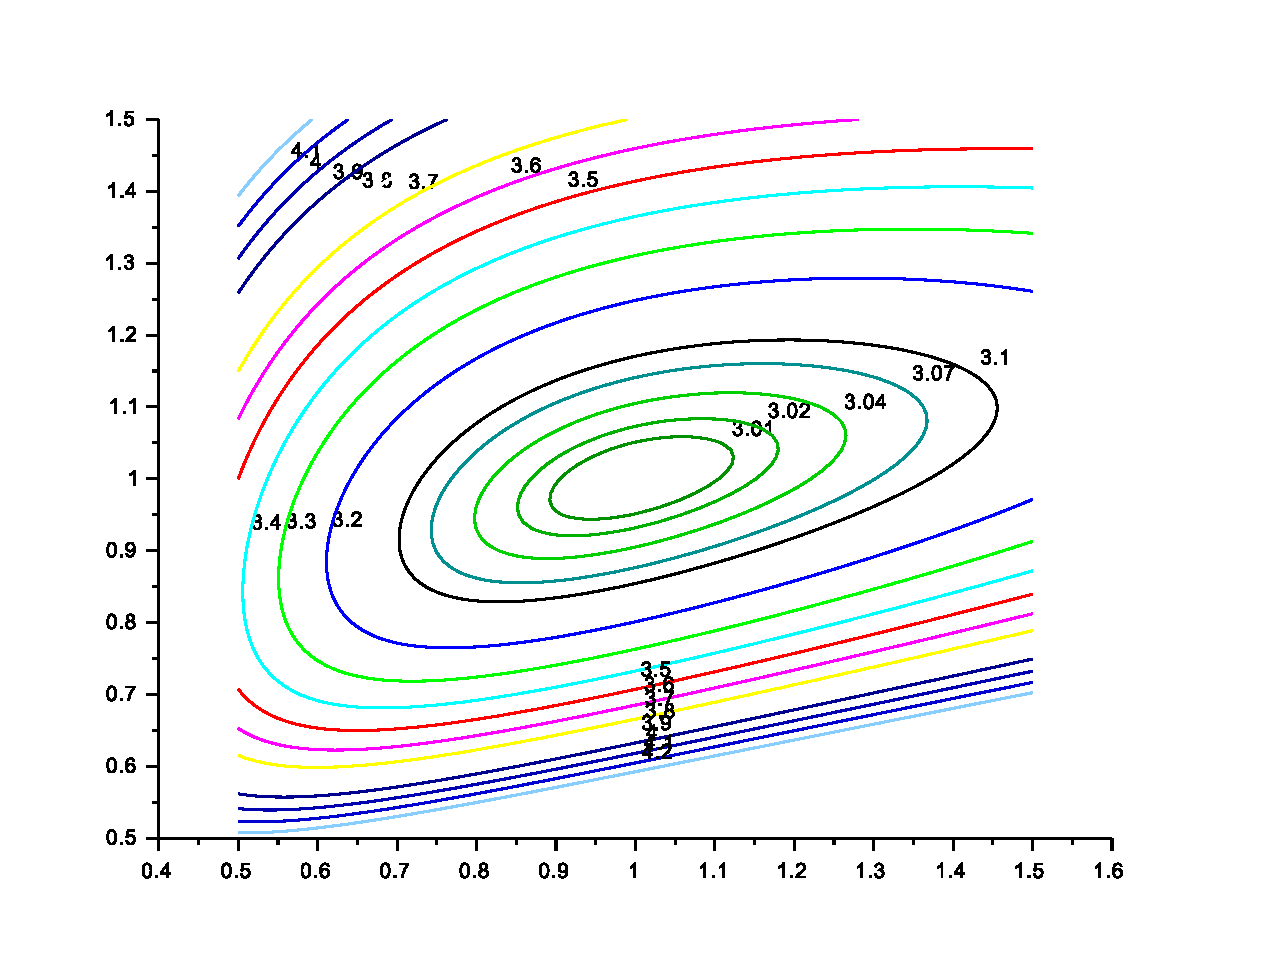
\includegraphics[width=10cm,height=10cm]{../Figures/ECRICOME_2019/Ecricome_2019_figure1.pdf}
  \end{center}
  Établir une conjecture à partir du graphique quant à l'existence
  d'un extremum local pour $f$, dont on donnera la nature, la valeur
  approximative et les coordonnées du point en lequel il semble être
  atteint.
  
  \begin{proof}~%
    \begin{noliste}{$\sbullet$}
    \item Le graphique fait apparaître les lignes de niveau de la
      fonction $f$. Ces courbes relient les points $(x, y) \in \R^2$
      pour lesquels la fonction $f$ prend la même valeur. Sur la
      représentation, on constate que la fonction $f$ prend des
      valeurs de plus en plus grande en s'écartant du point $(1,
      1)$. %

    \item De plus, en ce point, la valeur de la fonction $f$ est :
      \[
      f(1, 1) \ = \ \dfrac{1}{1^2} + 1^2 + \dfrac{1}{1} \ = \ 3
      \]
      Cette valeur est plus faible que les valeurs des lignes de
      niveau apparaissant sur le graphique. %
    \end{noliste}
    \concL{On peut émettre la conjecture que la fonction $f$ admet un
      minimum local, de valeur $3$, au point $(1, 1)$.}{15.4}~\\[-1.2cm]
  \end{proof}


  \newpage


\item
  \begin{noliste}{a)}
    \setlength{\itemsep}{2mm}
  \item Démontrer que $f$ est de classe $\Cont{2}$ sur $\R_+^{*}
    \times \R_+^{*}$.
    
    \begin{proof}~\\%
      La fonction $f$ est de classe $\Cont{2}$ sur $\R_+^{*} \times
      \R_+^{*}$ car est la somme $f = f_1 + f_2 + f_3$ des fonctions :
      \begin{noliste}{$\stimes$}
      \item $f_1 : (x, y) \mapsto \dfrac{x}{y^2}$ de classe $\Cont{2}$
        sur $\R_+^{*} \times \R_+^{*}$ en tant que quotient de
        fonctions de deux variables polynomiales dont le dénominateur
        ne s'annule pas sur $\R_+^{*} \times \R_+^{*}$.

      \item $f_2 : (x, y) \mapsto y^2$ de classe $\Cont{2}$ sur
        $\R_+^{*} \times \R_+^{*}$ en tant que fonction de deux
        variables polynomiale.

      \item $f_3 : (x, y) \mapsto \dfrac{1}{x}$ de classe $\Cont{2}$
        sur $\R_+^{*} \times \R_+^{*}$ en tant qu'inverse d'une
        fonction de deux variables polynomiale qui ne s'annule pas sur
        $\R_+^{*} \times \R_+^{*}$.
      \end{noliste}
      \conc{La fonction $f$ est bien de classe $\Cont{2}$ sur
        $\R_+^{*} \times \R_+^{*}$.}
      \begin{remarkL}{.98}
        \begin{noliste}{$\sbullet$}
        \item Il est important de noter que les fonctions $f_2$ et
          $f_3$ sont bien des fonctions de deux variables même si leur
          expression n'en fait apparaître qu'une. Considérer les
          fonctions $y \mapsto y^2$ et $x \mapsto \dfrac{1}{x}$
          démontre un manque de compréhension des objets utilisés et
          est donc sanctionné.
        \item Il en est de même pour chacune des deux fonctions du
          quotient définissant $f_1$.\\
          Plus précisément, cette fonction est le quotient : $f_1 =
          \dfrac{h_1}{h_2}$ de :
          \begin{noliste}{$\stimes$}
          \item $h_1 : (x, y) \mapsto x$ qui est une fonction de deux
            variables polynomiale.
          \item $h_2 : (x, y) \mapsto y^2$ qui est une fonction de deux
            variables polynomiale.            
          \end{noliste}
          Rappelons qu'une fonction de deux variables polynomiale est
          une fonction apparaissant comme combinaison linéaire de
          fonctions monomiales (fonctions de la forme $(x, y) \mapsto
          x^r \, y^s$ avec $(r, s) \in \N \times \N$).
        \end{noliste}
      \end{remarkL}~\\[-1.4cm]
    \end{proof}

  \item Calculer les dérivées partielles premières de $f$, puis
    démontrer que $f$ admet un unique point critique, noté $A$, que
    l'on déterminera.

    \begin{proof}~%
      \begin{noliste}{$\sbullet$}
      \item La fonction $f$ est de classe $\Cont{1}$ sur $\R_+^{*}
        \times \R_+^{*}$. \\
        Elle admet donc des dérivées partielles premières sur cet
        ensemble.

      \item Soit $(x, y) \in \R_+^{*} \times \R_+^{*}$. Tout d'abord
        : %
        \[
        \dfn{f}{1}(x, y) \ = \ \dfrac{1}{y^2} - \dfrac{1}{x^2}
        \]
        Par ailleurs : 
        \[
        \dfn{f}{2}(x, y) \ = \ -\dfrac{2x}{y^3} + 2 y
        \]
        \conc{$\dfn{f}{1}(x, y) \ = \ \dfrac{1}{y^2} - \dfrac{1}{x^2}$
          \quad et \quad $\dfn{f}{2}(x, y) \ = \ -\dfrac{2x}{y^3} + 2
          y$}

      \item D'autre part :
        \[
        \text{$(x, y)$ est un point critique de $f$} \ \Leftrightarrow
        \ \nabla(f)(x, y) = 0_{\M{2,1}} \ \Leftrightarrow \ \left\{
          \begin{array}{l}
            \dfn{f}{1}(x, y) \ = \ 0
            \\[.2cm]
            \dfn{f}{2}(x, y) \ = \ 0
          \end{array}
        \right.
        \]
        % Ainsi :
        \[
        \begin{array}[t]{R{.8cm}C{3.4cm}cl@{\qquad}>{\it}R{6.4cm}}
          Ainsi : & $(x, y)$ est un point critique de $f$ 
          & \Leftrightarrow & 
          \left\{
            \begin{array}{rcl}
              \dfrac{1}{y^2} - \dfrac{1}{x^2} & = & 0
              \\[.5cm]
              -\dfrac{2x}{y^3} + 2 y & = & 0
            \end{array}
          \right.
          \\[1.2cm]
          & & \Leftrightarrow & 
          \left\{
            \begin{array}{rcl}
              \dfrac{1}{y^2} & = & \dfrac{1}{x^2}
              \\[.4cm]
              \bcancel{2} y & = & \dfrac{\bcancel{2} \, x}{y^3}
            \end{array}
          \right.
          \\[1.2cm]
          & & \Leftrightarrow & 
          \left\{
            \begin{array}{rcl}
              y & = & x
              \\[.2cm]
              y & = & \dfrac{x}{y^3}
            \end{array}
          \right.
          & (car la fonction $x \mapsto \dfrac{1}{x^2}$ réalise
          \\[.2cm]
          une bijection de $\R_+^*$ dans $\R_+^*$)
          \nl
          \nl%[-.2cm]
          & & \Leftrightarrow & 
          \left\{
            \begin{array}{rcl}
              y & = & x
              \\[.2cm]
              x & = & \dfrac{x}{x^3}
            \end{array}
          \right.
          & (en remplaçant $y$ par $x$ dans la seconde équation)
          \nl
          \nl%[-.2cm]
          & & \Leftrightarrow & 
          \left\{
            \begin{array}{rcl}
              y & = & x
              \\[.2cm]
              x & = & \dfrac{1}{x^2}
            \end{array}
          \right.
          \\[.8cm]
          & & \Leftrightarrow & 
          \left\{
            \begin{array}{rcl}
              y & = & x
              \\[.2cm]
              x^3 & = & 1
            \end{array}
          \right.
          \\[.8cm]
          & & \Leftrightarrow & 
          \left\{
            \begin{array}{rcl}
              y & = & x
              \\[.1cm]
              x & = & 1
            \end{array}
          \right.
          & (car la fonction $x \mapsto x^3$ réalise \\
          une bijection de $\R$ dans $\R$)
        \end{array}
        \]
        \concL{On en déduit que la fonction $f$ admet comme unique
          point critique le point $A$ de coordonnées $(1, 1)$.}{15.4}
      \end{noliste}
      \begin{remarkL}{.98}%~%
        \begin{noliste}{$\sbullet$}
        \item La difficulté de cette question réside dans le fait
          qu'il n'existe pas de méthode générale pour résoudre
          l'équation $\nabla(f)(x,y) = 0_{\M{2,1}}$.\\
          On est donc confronté à une question bien plus complexe
          qu'une résolution de système d'équations linéaires (que l'on
          résout aisément à l'aide de la méthode du pivot de Gauss).
        \item Lors de la recherche de points critiques, on doit faire
          appel à des méthodes ad hoc. Il est par exemple assez
          fréquent de faire apparaître une équation du type :
          \[
          \varphi(x) = \varphi(y)
          \]
          où $\varphi : \R \to \R$ est une fonction bijective. En
          réalité, c'est le caractère injectif ($\varphi$ est
          strictement monotone sur $\R$ par exemple) qui nous
          intéresse ici puisqu'il permet de conclure : 
          \[
          x = y
          \]
          En injectant cette égalité $x = y$ dans la seconde équation,
          on obtient une nouvelle équation qui ne dépend plus que
          d'une variable et qu'il est donc plus simple de résoudre.\\[.1cm]
          C'est la stratégie utilisée ici avec la fonction $\varphi :
          x \mapsto \dfrac{1}{x^2}$ qui est strictement décroissante
          (et donc injective) sur $\R_+^*$.
        \end{noliste}
      \end{remarkL}


      \newpage


      \begin{remarkL}{.98}%~%
        \begin{noliste}{$\sbullet$}
        \item Il est aussi possible de détailler, pas à pas,
          l'équivalence $\dfrac{1}{y^2} = \dfrac{1}{x^2} \
          \Leftrightarrow \ y = x$.\\
          Plus précisément :
          \[
          \dfrac{1}{y^2} = \dfrac{1}{x^2} \ \Leftrightarrow \ y^2 =
          x^2 \ \Leftrightarrow \ \sqrt{y^2} = \sqrt{x^2} \
          \Leftrightarrow \ |y| = |x| \ \Leftrightarrow \ y = x
          \]
          La dernière étape est obtenue par le caractère positif de
          $x$ et de $y$.

        \item Détaillons enfin la dernière étape de résolution de la
          question.
          \[
          x^3 = 1 \ \Leftrightarrow \ x^3 - 1 = 0 \ \Leftrightarrow \
          (x - 1) (x^2 + x + 1) = 0 \ \Leftrightarrow \ \text{$x = 1$
            $\OU{}$ $x^2 + x + 1 = 0$}
          \]
          Or le polynôme $P(X) = X^2 + X + 1$ n'admet pas de racine
          réelle car il est de discriminant $\Delta = 1 - 4 = -3 <
          0$. On en déduit : $x^3 = 1 \ \Leftrightarrow \ x =
          1$.

        \item On a opté pour une rédaction différente. Détaillons
          l'argument utilisé. On cherche à résoudre $\psi(x) = 1$ où
          $\psi : x \mapsto x^3$. Cette équation admet comme solution
          évidente $x = 1$ et c'est l'unique solution car la fonction
          $\psi$ réalise une bijection de $\R$ dans $\R$ (encore une
          fois, le caractère injectif suffisait ici).
        \end{noliste}
      \end{remarkL}~\\[-1.6cm]
    \end{proof}
    
  \item Calculer les dérivées partielles secondes de $f$, puis
    démontrer que la matrice hessienne de $f$ au point $A$ est la
    matrice $H$ définie par : $H \ = \
    \begin{smatrix}
      2 & -2\\
      -2 & 8
    \end{smatrix}$.

    \begin{proof}~%
      \begin{noliste}{$\sbullet$}
      \item La fonction $f$ est de classe $\Cont{2}$ sur $\R_+^*
        \times \R_+^*$.\\
        Elle admet donc des dérivées partielles d'ordre $2$ sur $\R_+^*
        \times \R_+^*$.

      \item Soit $(x, y) \in \R_+^* \times \R_+^*$. Tout d'abord :
        \[
        \ddfn{f}{11}(x, y) \ = \ -\dfrac{-2}{x^3} \ = \ \dfrac{2}{x^3}
        \]

      \item Ensuite :
        \[
        \ddfn{f}{12}(x, y) \ = \ -\dfrac{2}{y^3} \ = \ \ddfn{f}{21}(x,
        y)
        \]
        La dernière égalité est obtenue en vertu du théorème de
        Schwarz puisque la fonction $f$ est $\Cont{2}$ sur l'{\bf
          ouvert} $\R_+^* \times \R_+^*$.
        
      \item Enfin :        
        \[
        \ddfn{f}{22}(x, y) \ = \ -2x \ \dfrac{-3}{y^4} + 2 \ = \
        \dfrac{6x}{y^4} + 2
        \]
      \end{noliste}
      \concL{Pour tout $(x, y) \in \R_+^* \times \R_+^*$, \
        $\ddfn{f}{11}(x, y) \ = \ \dfrac{2}{x^3}$, \ \
        $\ddfn{f}{12}(x, y) \ = \ -\dfrac{2}{y^3} \ = \
        \ddfn{f}{21}(x, y)$
        \\[.2cm]
        et $\ddfn{f}{22}(x, y) \ = \ \dfrac{6x}{y^4} +
        2$.}{15.4}%~\\[-1cm]
      \begin{remarkL}{1}%~%
        \begin{noliste}{$\sbullet$}
        \item Il faut penser à utiliser le théorème de Schwarz dès que
          la fonction à deux variables considérée est $\Cont{2}$ sur
          un ouvert $U \subset \R^2$.
        \item Ici, le calcul de $\ddfn{f}{12}(x, y)$ et
          $\ddfn{f}{21}(x, y)$ est aisé. Il faut alors concevoir le
          résultat du théorème de Schwarz comme une mesure de
          vérification : en dérivant par rapport à la $\ere{1}$
          variable puis par rapport à la $\eme{2}$, on doit obtenir le
          même résultat que dans l'ordre inverse.
        \end{noliste}      
      \end{remarkL}


      \newpage


      \noindent
      \begin{noliste}{$\sbullet$}
      \item On rappelle que la matrice hessienne de $f$ en un point
        $(x, y) \in \R_+^* \times \R_+^*$ est :
        \[
        \nabla^2(f)(x, y) =
        \begin{smatrix}
          \ddfn{f}{11}(x, y) & \ddfn{f}{12}(x, y) 
          \\[.6cm]
          \ddfn{f}{21}(x, y) & \ddfn{f}{22}(x, y) 
        \end{smatrix}
        = 
        \begin{smatrix}
          \dfrac{2}{x^3} & -\dfrac{2}{y^3}
          \\[.4cm]
          -\dfrac{2}{y^3} & \dfrac{6x}{y^4} + 2
        \end{smatrix}
        \]
        
      \item On en déduit : 
        \[
        H = \nabla^2(f)(1, 1) =
        \begin{smatrix}
          \dfrac{2}{1^3} & -\dfrac{2}{1^3}
          \\[.4cm]
          -\dfrac{2}{1^3} & \dfrac{6}{1^4} + 2
        \end{smatrix}        
        \]
      \end{noliste}
      \conc{$H =
        \begin{smatrix}
          2 & -2 \\[.2cm]
          -2 & 8
        \end{smatrix}$}~\\[-1cm]
    \end{proof}

  \item En déduire que la fonction $f$ admet au point $A$ un extremum
    local, préciser si cet extremum est un minimum, et donner sa
    valeur.


    \begin{proof}~\\%
      Soit $\lambda \in \R$. Rappelons tout d'abord que, pour toute
      matrice $H \in \M{2}$ :
      \[
      \begin{array}{R{4.8cm}cR{4.6cm}}
        $\lambda$ est une valeur propre de $H$ & \Leftrightarrow & $H
        - \lambda \ I$ n'est pas inversible        
        \nl
        \nl[-.2cm]
        & \Leftrightarrow & $\det(H - \lambda \ I) = 0$
      \end{array}
      \]

      \begin{noliste}{$\sbullet$}
      \item Or :
        \[
        \begin{array}{rcl}
          \det\Big(\nabla^2(f)(1, 1) - \lambda \ I\Big) & = & \det\left( 
            \begin{smatrix}
              2 - \lambda & -2 \\[.2cm]
              -2 & 8 - \lambda
            \end{smatrix} 
          \right)
          \\[.6cm]
          & = & (2 - \lambda)(8 - \lambda) - (-2)^2
          \\[.2cm]
          & = & (16 - 10 \, \lambda + \lambda^2) - 4
          \\[.2cm]
          & = & 12 - 10 \, \lambda + \lambda^2
        \end{array}
        \]
        Le polynôme $P(X) = 12 - 10 \, X + X^2$ admet pour
        discriminant :
        \[
        \Delta = (-10)^2 - 4 \times 12 = 100 - 48 = 52 > 0
        \]
        Ainsi, $P$ admet deux racines distinctes :
        \[
        \lambda_1 = \dfrac{10 + \sqrt{52}}{2} = \dfrac{10 + 2 \,
          \sqrt{13}}{2} = 5 + \sqrt{13} \qquad \text{ et } \qquad
        \lambda_2 = \dfrac{10 - \sqrt{52}}{2} = \dfrac{10 - 2 \,
          \sqrt{13}}{2} = 5 - \sqrt{13}
        \]        
        Enfin, comme $13 < 16$, on a : $\sqrt{13} \ < \ \sqrt{16} \ =
        \ 4$ et $-\sqrt{13} > -4$. On en déduit :
        \[
        \lambda_2 = 5 - \sqrt{13} > 5-4 = 1 > 0
        \]
        \concL{Ainsi, $\nabla^2(f)(1, 1)$ admet pour valeurs propres
          $\lambda_1 = 5 + \sqrt{13} > 0$ et $\lambda_2 > 0$.\\
          La fonction $f$ admet donc un minimum local au point $(1,
          1)$.}{14.4}~\\[-1.4cm]
      \end{noliste}
    \end{proof}
  \end{noliste}
\end{noliste}

\subsection*{Partie B} 

\noindent
Pour tout entier $n$ non nul, on note $h_n$ la fonction définie sur
$\R_+^{*}$ par :
\[
\forall x >0, \ \ h_n(x) \ = \ f(x^n,1) \ = \ x^n + 1 + \dfrac{1}{x^n}
\]
\begin{noliste}{1.}
  \setlength{\itemsep}{4mm} %
  \setcounter{enumi}{2}
\item Démontrer que pour tout entier naturel $n$ non nul, la fonction
  $h_n$ est strictement décroissante sur $]0,1[$ et strictement
  croissante sur $[1,+\infty[$.
  
  \begin{proof}~\\%
    Soit $n \in \N^*$.
    \begin{noliste}{$\sbullet$}
    \item La fonction $h_n$ est dérivable sur $\R_+^*$ car elle est la
      somme des fonctions :
      \begin{noliste}{$\stimes$}
      \item $x \mapsto x^n + 1$ dérivable sur $\R_+^*$ car
        polynomiale.

      \item $x \mapsto \dfrac{1}{x^n}$ dérivable sur $\R_+^*$ en tant
        qu'inverse de la fonction $x \mapsto x^n$ :
        \begin{noliste}{$-$}
        \item dérivable sur $\R_+^*$ car polynomiale,
        \item et qui ne s'annule pas sur $\R_+^*$.
        \end{noliste}        
      \end{noliste}

    \item Soit $x \in \R_+^*$.
      \[
      h_n'(x) \ = \ n \, x^{n-1} - \dfrac{n}{x^{n+1}} \ = \ n \
      \dfrac{x^{2n} - 1}{x^{n+1}}
      \]
      Comme $n > 0$ et $x^{n+1} > 0$, la quantité $h_n'(x)$ est du
      signe de $x^{2n} - 1$. On en déduit :
      \[
      h_n'(x) > 0 \ \Leftrightarrow \ x^{2n} - 1 > 0 \ \Leftrightarrow
      \ x^{2n} > 1  \ \Leftrightarrow \ x > 1
      \]
      La dernière équivalence est obtenue par stricte croissance de la
      fonction $x \mapsto x^{2n}$ sur $\R_+^*$.

    \item On en déduit le tableau de variations suivant.\\[-.2cm]
      \begin{center}
        \begin{tikzpicture}[scale=.8, transform shape] %
          \tkzTabInit[lgt=4,espcl=4] %
          {$x$ /1, %
            Signe de $h_n'(x)$ /1, %
            Variations de $h_n$ /2} %
          {$0$, $1$, $+\infty$}%
          \tkzTabLine{ d, -, z, +, }%
          \tkzTabVar{D+/$+\infty$, -/$3$, +/$+\infty$}%
          % \tkzTabIma{1}{3}{2}{$1$} %
        \end{tikzpicture}
      \end{center}
    \end{noliste}
    \begin{remarkL}{.98}%
      Afin de déterminer le signe de la quantité $x^{2n}-1$, on
      pouvait rédiger autrement.
      \begin{noliste}{$\sbullet$}
      \item Une première méthode consiste à étudier la fonction $g_n :
        x \mapsto x^{2n}-1$.\\
        Cette fonction étant polynomiale, elle est dérivable sur $\R$
        et pour tout $x \in \R_+^*$ :
        \[
        g_n'(x) \ = \ 2n\, x^{2n-1} > 0
        \]
        ~\\[-.7cm]
        La fonction $g_n$ est donc strictement croissante sur $]0,
        +\infty[$. Enfin, comme $g_n(1) = 0$ :
        \[
        \forall x \in \ ]0, 1[, \ x^{2n}-1 < 0 \qquad \text{ et }
        \qquad \forall x \in \ ]1, +\infty[, \ x^{2n}-1 > 0
        \]
        ~\\[-1.3cm]
      \item Une deuxième méthode consiste à factoriser $x^{2n}-1$ :
        \[
        x^{2n}-1 \ = \ \big( x^{n} \big)^2 - 1^2 \ = \ (x^n - 1) \,
        (x^n + 1)
        \]
        ~\\[-.7cm]
        Comme $x> 0$, alors $x^n > 0$ et $x^n + 1 > 0$. Le signe de
        $x^{2n}-1$ est donc celui de $x^n - 1$. Or :
        \[
        x^n - 1 \ = \ (x-1) (1 + x + \ldots + x^{n-1}) % \ = \ (x-1) \
        % \left( \Sum{k=0}{n-1} x^k \right)
        \]
        ~\\[-.7cm]
        Comme $1 + x + \ldots + x^{n-1} > 0$, le signe de $x^n - 1$
        (et donc de $x^{2n} - 1$) est celui de $x -1$.
      \end{noliste}
    \end{remarkL}~\\[-1.7cm]
  \end{proof}


  \newpage


\item En déduire que pour tout entier $n$ non nul, l'équation $h_n(x)
  = 4$ admet exactement deux solutions, notées $u_n$ et $v_n$ et
  vérifiant : $0 < u_n < 1 <v_n$.

    \begin{proof}~\\%
      Soit $n \in \N^*$.
      \begin{noliste}{$\sbullet$}
      \item La fonction $h_n$ est :
        \begin{noliste}{$\stimes$}
        \item continue sur $]0, 1[$,
        \item strictement décroissante sur $]0, 1[$.          
        \end{noliste}
        Elle réalise donc une bijection de $]0, 1[$ sur $h_n\big(]0,
        1[ \big)$. Or :
        \[
        h_n\big(]0, 1[ \big) \ = \ ]h_n(1), \dlim{x \tend 0} h_n(x)[ \
        = \ ]3, +\infty[
        \]
        Comme $4 \in \ ]3, +\infty[$, l'équation $h_n(x) = 4$ admet
        une unique solution sur $]0, 1[$.\\
        On note $u_n$ cette solution.

      \item De même, la fonction $h_n$ est :
        \begin{noliste}{$\stimes$}
        \item continue sur $]1, +\infty[$,
        \item strictement croissante sur $]1, +\infty[$.
        \end{noliste}
        Elle réalise donc une bijection de $]1, +\infty[$ sur
        $h_n\big( ]1, +\infty[ \big)$. Or :
        \[
        h_n\big( ]1, +\infty[ \big) \ = \ ]h_n(1), \dlim{x \tend
          +\infty} h_n(x)[ \ = \ ]3, +\infty[
        \]
        Comme $4 \in \ ]3, +\infty[$, l'équation $h_n(x) = 4$ admet
        une unique solution sur $]1, +\infty[$.\\
        On note $v_n$ cette solution.

      \item On remarque enfin : $h_n(1) \ = \ 3 \ \neq \ 4$. Ainsi, $x
        = 1$ n'est pas solution de l'équation $h_n(x) = 4$.%
        \concL{Pour tout entier $n$ non nul, l'équation $h_n(x) = 4$
          admet exactement deux solutions, notées $u_n$ et $v_n$ et
          vérifiant : $0 < u_n < 1 <v_n$.}{15.4}~\\[-1.3cm]
      \end{noliste}
    \end{proof}
  
\item
  \begin{noliste}{a)}
    \setlength{\itemsep}{2mm}
  \item Démontrer :
    \[
    \forall x > 0, \ \forall n \in \N^*, \ h_{n+1}(x) - h_n(x) = 
    \dfrac{(x-1)(x^{2n+1}-1)}{x^{n+1}}
    \]
    
    \begin{proof}~\\%
      Soit $x > 0$ et soit $n \in \N^*$.
      \[
      \begin{array}{rcl@{\qquad}>{\it}R{5.3cm}}
        h_{n+1}(x) - h_n(x) 
        & = & \left( x^{n+1} + \bcancel{1} + \dfrac{1}{x^{n+1}}
        \right) - \left( x^{n} + \bcancel{1} + \dfrac{1}{x^{n}}
        \right)  
        \\[.6cm]
        & = & \dfrac{x^{2n+2} +1}{x^{n+1}} - \dfrac{x^{2n+1}
          +x}{x^{n+1}} 
        \\[.6cm]
        & = & \dfrac{x^{2n+2} - x^{2n+1} - (x -1)}{x^{n+1}}
        \\[.6cm]
        & = & \dfrac{x^{2n+1} \, (x - 1) - (x -1)}{x^{n+1}}
        % \\[.6cm]
        \ = \ \dfrac{(x-1)(x^{2n+1} - 1)}{x^{n+1}}
      \end{array}
      \]
      \conc{$\forall x > 0, \ \forall n \in \N^*, \ h_{n+1}(x) -
        h_n(x) = \dfrac{(x-1)(x^{2n+1}-1)}{x^{n+1}}$}~\\[-.8cm]
    \end{proof}


    \newpage


  \item En déduire : $\forall n \in \N^*, \ h_{n+1}(v_n) \geq 4$.

    \begin{proof}~\\%
      Soit $n \in \N^*$.
      \begin{noliste}{$\sbullet$}
      \item D'après la question précédente, pour tout $x > 0$ :
        \[
        h_{n+1}(x) - h_n(x) \ = \ \dfrac{(x-1)(x^{2n+1}-1)}{x^{n+1}}
        \]
        Comme $x > 0$ alors $x^{n+1} > 0$. Ainsi, la quantité
        $h_{n+1}(x) - h_n(x)$ est du signe du produit
        $(x-1)(x^{2n+1}-1)$. Notons alors que pour tout $x > 1$,
        $x^{2n+1}-1 > 0$ (vu précédemment).%
        \conc{Ainsi : $\forall n \in \N^*, \ \forall x > 1, \
          h_{n+1}(x) - h_n(x) > 0$.}
        
      \item On applique l'inégalité précédente à $v_n > 1$ (d'après la
        question \itbf{4.}). On obtient :
        \[
        h_{n+1}(v_n) - h_n(v_n) > 0 \quad \text{ ou encore } \quad
        h_{n+1}(v_n) > h_n(v_n) = 4
        \]
        \conc{On a bien : $\forall n \in \N^*, \ h_{n+1}(v_n) \geq
          4$.}~\\[-1.5cm]
      \end{noliste}
    \end{proof}
    
  \item Montrer alors que la suite $(v_n)$ est décroissante.

    \begin{proof}~\\%
      Soit $n \in \N^*$.
      \begin{noliste}{$\sbullet$}
      \item Par définition de $v_{n+1}$, on a : $h_{n+1}(v_{n+1}) =
        4$. Ainsi, d'après la question précédente :
        \[
        h_{n+1}(v_{n}) \ \geq \ h_{n+1}(v_{n+1}) 
        \]

      \item De plus, on sait d'après la question \itbf{4.} que :
        \begin{noliste}{$\stimes$}
        \item $v_n > 1$ et $v_{n+1} > 1$,
        \item la fonction $h_{n+1}$ réalise une bijection de $]1,
          +\infty[$ sur $]3, +\infty[$.          
        \end{noliste}
        La réciproque de cette bijection, définie de $]3, +\infty[$
        sur $]1, +\infty[$ est strictement croissante car de même
        monotonie que $h_{n+1}$ sur $]1, +\infty[$. En l'appliquant de
        part et d'autre de l'inégalité : %précédente, on obtient :
        \[
        v_n \ \geq \ v_{n+1}
        \]
      \end{noliste}
      \conc{On en conclut : $\forall n \in \N^*$, $v_n \ \geq \
        v_{n+1}$. La suite $(v_n)$ est donc décroissante.}~\\[-1.1cm]
      \begin{remarkL}{1}%~
        \begin{noliste}{$\sbullet$}
        \item La {\bf Partie B} consiste en l'étude de la suite
          $(v_n)$. On parle ici de \og suite implicite \fg{} car on
          n'a pas accès à la définition explicite de la suite $(v_n)$
          mais simplement à la propriété qui permet de définir chacun
          de ses termes, à savoir :
          \[
          \begin{array}{R{14cm}}
            Pour tout $n \in \N^*$, $v_n$ est l'unique racine de
            l'équation $h_n(x) = 4$ sur $]1, +\infty[$
          \end{array}
          \]
          On comprend alors que l'étude de $(v_n)$ va passer par l'étude
          des propriétés de la fonction $h_n$.

        \item De cette définition, on tire la propriété :
          $\Boxed{\forall m \in \N^*, \ h_m(v_m) = 4}$.\\
          Cette propriété est au c\oe{}ur de l'étude de la suite
          implicite $(v_n)$.\\
          On l'utilise en \itbf{5.b)} pour $m = n$ et en \itbf{5.c)}
          pour $m = n+1$.

        \item Comme la suite $(v_n)$ est définie de manière implicite,
          on n'étudie pas la monotonie de $(v_n)$ à l'aide de la
          différence $v_{n+1} - v_n$. Il est par contre très classique
          de passer par l'inégalité : 
          \[
          h_{n+1}(v_n) \ \geq \ h_{n+1}(v_{n+})
          \]
          et de conclure : $v_n \ \geq \ v_{n+1}$ à l'aide d'une
          propriété de $h_{n+1}$.
        \end{noliste}
      \end{remarkL}~\\[-1.6cm]
    \end{proof}
  \end{noliste}
  

  \newpage


\item 
  \begin{noliste}{a)}
    \setlength{\itemsep}{2mm}
  \item Démontrer que la suite $(v_n)$ converge vers un réel $\ell$ et
    montrer : $\ell \geq 1$.

    \begin{proof}~\\%
      La suite $(v_n)$ est :
      \begin{noliste}{$\stimes$}
      \item décroissante d'après la question \itbf{5.c)},
      \item minorée par $1$ ($\forall n \in \N^*$, $v_n > 1$) d'après
        la question \itbf{4}.        
      \end{noliste}
      \conc{On en conclut que la suite $(v_n)$ converge vers un réel
        $\ell \geq 1$.}~\\[-1.2cm]
    \end{proof}
    
  \item En supposant que $\ell > 1$, démontrer : $\dlim{n \to +\infty}
    v_n^n = +\infty$.\\
    En déduire une contradiction.

    \begin{proof}~\\%
      Dans cette question, on suppose $\ell > 1$.
      \begin{noliste}{$\sbullet$}
      \item Comme $\ell \neq 0$, on a : $v_n \eqn{} \ell$. Ainsi :
        \[
        (v_n)^n \eqn{} \ell^n \tendn +\infty \quad \text{\it (car
          $\ell > 1$)}
        \]
        \conc{On a bien : $\dlim{n \tend +\infty} (v_n)^n = +\infty$.}
        \begin{remark}%
          Comme la suite $(v_n)$ est à termes strictement positifs, on
          pouvait aussi écrire :
            \[
            (v_n)^n \ = \ \exp\big( n \, \ln(v_n) \big)
            \]
            Puis : $\ln(v_n) \eqn{} \ln(\ell)$ puisque $\ell \neq
            1$.\\
            Ainsi : $n \, \ln(v_n) \eqn{} n \, \ell \tend +\infty$ car
            $\ell > 0$. Et enfin, par composition de limites :
            \[
            \dlim{n \tend +\infty} \exp\big( n \, \ln(v_n) \big) \ = \
            +\infty
            \]
        \end{remark}

      \item Remarquons alors : 
        \[
        h_n(v_n) \ = \ (v_n)^n + 1 + \dfrac{1}{(v_n)^n}
        \]
        Comme $\dlim{n \tend +\infty} (v_n)^n = +\infty$, on en
        conclut : 
        \[
        \dlim{n \tend +\infty} h_n(v_n) = +\infty
        \]
        Or, par définition de la suite $(v_n)$, pour tout $n \in
        \N^*$, $h_n(v_n) = 4$ et ainsi :
        \[
        \dlim{n \tend +\infty} h_n(v_n) = 4
        \]
        Contradiciton !
      \end{noliste}
        \begin{remark}
          C'est encore une fois la propriété de définition des termes
          de la suite $(v_n)$ qui est utilisée ici ($\forall n \in
          \N^*$, $h_n(v_n) = 4$). On insiste sur le fait que cette
          propriété est fondamentale pour l'étude de la suite
          implicite $(v_n)$.
        \end{remark}~\\[-1.6cm]
    \end{proof}


    \newpage

    
  \item Déterminer la limite de $(v_n)$.

    \begin{proof}~%
      \begin{noliste}{$\sbullet$}
      \item En question \itbf{6.a)}, on a démontré que la suite
        $(v_n)$ converge vers un réel $\ell \geq 1$.

      \item En question \itbf{6.b)}, on a démontré que l'hypothèse
        $\ell > 1$ menait à une contradiction.\\
        On en conclut que sa négation est vérifiée, à savoir : $\ell
        \leq 1$.

      \end{noliste}
      \conc{Ainsi, la suite $(v_n)$ converge ver $\ell = 1$.}~\\[-1.2cm]
      \begin{remark}%
        L'énoncé donne les réponses aux questions \itbf{6.a)} et
        \itbf{6.b)}. Il est donc possible de traiter la question
        \itbf{6.c)}, question bilan, sans avoir réussi à traiter les
        questions précédentes.
      \end{remark}~\\[-1.6cm]
    \end{proof}
  \end{noliste}
  
\item
  \begin{noliste}{a)}
    \setlength{\itemsep}{2mm}
  \item Montrer : $\forall n \geq 1, \ v_n \leq 3$.

    \begin{proof}~\\%
      Soit $n \in \N^*$.
      \begin{noliste}{$\sbullet$}
      \item Rappelons tout d'abord : $v_n > 1$ (question
        \itbf{4.}). D'autre part :
        \[
        \begin{array}{R{2cm}rcl@{\qquad}>{\it}R{5.3cm}}
          & v_n \leq 3 & \Leftrightarrow & h_n(v_n) \leq h_n(3)
          & (car $h_n$ est strictement croissante sur $]1, +\infty[$)
          \nl
          \nl[-.3cm]
          & & \Leftrightarrow & 4 \leq h_n(3)
          & (par définition de $v_n$)
        \end{array}
        \]

      \item Or, comme $3^n \geq 3$ (puisque $n > 0) $: 
        \[
        h_n(3) \ = \ 3^n + 1 + \dfrac{1}{3^n} \ \geq \ 3 + 1 +
        \dfrac{1}{3^n} > 4
        \]        
      \end{noliste}
      \conc{Pour tout $n \in \N^*$, on a bien : $h_n(3) \geq 4$ et
        donc $v_n \geq 3$.}~\\[-1.2cm]
      \begin{remarkL}{.98}
        \begin{noliste}{$\sbullet$}
        \item Encore une fois, c'est la propriété de définition des
          termes de la suite $(v_n)$ qui est utilisée ici. C'est
          logique puisqu'on ne connaît pas d'expression explicite des
          termes de $(v_n)$.

        \item La présence de la quantification \og $\forall n \in
          \N^*$ \fg{} peut faire penser à utiliser une récurrence. Ce
          type de raisonnement nécessite l'existence d'une propriété
          liant les termes de rangs successifs afin pouvoir mettre en
          \oe{}uvre l'étape d'hérédité. C'est pourquoi la récurrence
          est l'outil de base de démonstration des propriétés des
          suites récurrentes d'ordre $1$ (le terme au rang $n+1$
          s'exprime directement en fonction du terme au rang
          $n$). L'utilisation est plus rare dans le cas des suites
          implicites mais était possible dans cette question. En
          effet, comme la suite $(v_n)$ est décroissante, on sait que
          pour tout $n \in \N^*$ :
          \[
          v_{n+1} \leq v_n
          \]
          L'étape d'hérédité ne pose pas de problème.\\
          En effet, si l'on sait $v_n \leq 3$, on obtient alors, par
          transitivité : $v_{n+1} \leq v_n \leq 3$.\\
          Il reste alors à démontrer la propriété d'initialisation, à
          savoir $v_1 \leq 3$.\\
          Encore une fois, il faut revenir à la propriété de
          définition des termes de la suite $(v_n)$ :
          \[
          h_1(v_1) \ = \ v_1 + 1 + \dfrac{1}{v_1} \ = \ 4
          \]
          Ainsi : $v_1 \ = \ 3 - \frac{1}{v_1} \ \leq \ 3$ car $v_1 >
          0$ (question \itbf{4.)}).
        \end{noliste}

      \end{remarkL}~\\[-1.5cm]
    \end{proof}


    \newpage


  \item Écrire une fonction \Scilab{} d'en-tête {\tt function y =
      h(n,x)} qui renvoie la valeur de $h_n(x)$ lorsqu'on lui fournit
    un entier naturel $n$ non nul et un réel $x \in \R_+^{*}$ en
    entrée.

    \begin{proof}~%
      \begin{scilab}
        & \tcFun{function} \tcVar{y} = \underline{h}(\tcVar{n},
        \tcVar{x}) \nl % 
        & \quad y = x\puis{}n + 1 + (1 / x\puis{}n ) \nl %
        & \tcFun{endfunction}
      \end{scilab}~\\[-1cm]
      \begin{remark}%
        Il n'y a aucune difficulté à coder en \Scilab{} une fonction
        dont l'expression est donnée dans l'énoncé. Il est donc
        impensable de ne pas traiter cette question.
      \end{remark}~\\[-1.6cm]
    \end{proof}
        
  \item Compléter la fonction suivante pour qu'elle renvoie une valeur
    approchée à $10^{-5}$ près de $v_n$ par la méthode de dichotomie
    lorsqu'on lui fournit un entier $n \geq 1$ en entrée :
    \begin{scilab}
      & \tcFun{function} \tcVar{res} = \underline{v}(\tcVar{n}) \nl %
      & \quad a = 1 \nl %
      & \quad b = 3 \nl %
      & \quad \tcFor{while} (b-a) > 10\puis{}(-5) \nl %
      & \quad \quad c = (a+b) / 2 \nl %
      & \quad \quad \tcIf{if} h(\tcVar{n},c) < 4 \tcIf{then} \nl %
      & \quad \quad \quad ........ \nl %
      & \quad \quad \tcIf{else} \nl %
      & \quad \quad \quad ........ \nl %
      & \quad \quad \tcIf{end} \nl %
      & \quad \tcFor{end} \nl %
      & \quad .......... \nl %
      & \tcFun{endfunction}
    \end{scilab}

    \begin{proof}~\\%
%       \noindent Pour comprendre ce programme, commençons par rappeler
%       les différents éléments de l'algorithme de dichotomie.
      Commençons par rappeler le cadre de la recherche par
      dichotomie.\\[-.3cm] 
      \[
      \Boxed{
        \begin{array}{R{15cm}}
          \it Calcul approché d'un zéro d'une fonction par dichotomie
          \nl[.1cm] 
          {\bf Données} :
          \begin{noliste}{$\stimes$}
          \item une fonction $f : \R \to \R$,
          \item un intervalle de recherche $[a,b]$,
          \item une précision de recherche $\eps$.
          \end{noliste}
          \nl[-.2cm]
          {\bf Résultat} :  une valeur approchée à $\eps$ près d'un
          zéro (sur l'intervalle $[a, b]$) de la fonction $f$.\\[.1cm] 
          Autrement dit, une valeur approchée (à $\eps$ près) d'un
          réel $x \in [a, b]$ tel que : $f(x) = 0$.
        \end{array}
      }
      \]
      \begin{noliste}{$\sbullet$}
      \item La dichotomie est une méthode itérative dont le principe,
        comme son nom l'indique, est de découper à chaque itération
        l'intervalle de recherche en deux nouveaux
        intervalles. L'intervalle de recherche est découpé en son
        milieu. On obtient deux nouveaux intervalles :
        \begin{noliste}{$\stimes$}
        \item un intervalle dans lequel on sait que l'on va trouver un
          zéro de $f$. \\
          Cet intervalle est conservé pour l'itération suivante.
        \item un intervalle dans lequel ne se trouve pas forcément un
          zéro de $f$. \\
          Cet intervalle n'est pas conservé dans la suite de
          l'algorithme.
        \end{noliste}
        La largeur de l'intervalle de recherche est ainsi divisée par
        $2$ à chaque itération.\\
        On itère jusqu'à obtenir un intervalle $I$ contenant un zéro
        de $f$ et de largeur plus faible que $\eps$.\\
        Les points de cet intervalle $I$ sont tous de bonnes
        approximations du zéro contenu dans $I$.


        \newpage


      \item C'est le {\bf théorème des valeurs intermédiaires} qui
        permet de choisir l'intervalle qu'il faut garder à chaque
        étape. Rappelons son énoncé et précisons maintenant
        l'algorithme :
      \end{noliste}
      
      \begin{minipage}{.55\linewidth}
        \[
        \boxedhvv{0}{0.2}{0.2}{
          \begin{array}{R{9cm}}
            {\bf Théorème des Valeurs Intermédiaires}
            \begin{noliste}{}
            \item Soit $f : [a,b] \to \R$ continue sur
              l'\textbf{intervalle} $[a,b]$.
            \item Supposons : $f(a) \ f(b) \leq 0$.
            \end{noliste}
            Alors il existe $c \in [a, b]$ tel que $f(c) = 0$.
          \end{array}
        }
        \]
        \[
        \boxedhvv{0}{0.2}{0.4}{
          \begin{array}{R{9cm}}
            {\bf Calcul des suites $(a_m)$, $(b_m)$, $(c_m)$}\\[.2cm]
            \dashuline{Cas $f(a) \leq 0$ et $f(b) \geq 0$}
            \begin{noliste}{$\sbullet$}
            \item Initialement, $a_0 = a$, $b_0 = b$
              % , $c_0 = \dfrac{a_0+b_0}{2}$
            \item À chaque tour de boucle (tant que $b_m - a_m >
              \eps$) :
              \begin{liste}{$\stimes$}
              \item $c_{m} = \dfrac{a_{m} + b_{m}}{2}$ \quad (point milieu
                de $[a_m, b_m]$)
              \end{liste}
            \end{noliste}
            %\begin{multicols}{2}
            \begin{minipage}{.05\linewidth}
              ~
            \end{minipage}
            \begin{minipage}{.48\linewidth}
              \begin{liste}{$\stimes$}
              \item si $f(c_m) < 0$ alors :
                \begin{noliste}{$*$}
                \item $a_{m+1} = c_m$
                \item $b_{m+1} = b_m$
                \end{noliste}
              \end{liste}
            \end{minipage}
            \begin{minipage}{.42\linewidth}
              \begin{liste}{$\stimes$}
              \item si $f(c_m) \geq 0$ alors :
                \begin{noliste}{$*$}
                \item $a_{m+1} = a_m$
                \item $b_{m+1} = c_m$
                \end{noliste}
              \end{liste}
            \end{minipage}
                % \end{multicols}
          \end{array}
        }
        \]
      \end{minipage}
      \ \qquad \ 
      \begin{minipage}{.4\linewidth}
        \begin{center}
          %% French babel fout la merde : ne pas oublier shorthandoff
          \shorthandoff{;}
          \begin{tikzpicture}[scale = .65, %
            declare function = {f(\x) =
              -(\x+1)*(\x-sqrt(2)+.2)*(\x-9)/18;},] %
            \edef\a{0}. %
            \edef\cc{3}. %
            \edef\b{8}. %
            \def\bot{-6.3}. %
            \def\top{6.8}. %
            \draw[very thin,color=gray!50] (\a, \bot) grid (\b,
            \top); %
            \draw[-] (\a-.8,0) -- (\b+0.8,0) ; %
            \draw[-] (0,\bot) -- (0,\top) ; %
            \draw[-] (\b,\bot) -- (\b,\top) ; %
            \draw[color=blue, very thick, domain=\a:\b, samples = 60]
            plot (\x, {f(\x)}); %
            \draw[-, red, very thick] (\a,-2) node[left = 3pt] {$a_0$}
            -- (\b,-2) node[right = 3pt] {$b_0$}; %
            \pointG{\a}{-2}{.2}{red}; %
            \pointD{\b}{-2}{.2}{red}; %
            \foreach \x in {1,...,4} %
            { %
              \pgfmathparse{(\a+\b)/2}; %
              \xdef\cc{\pgfmathresult}; %
              \pgfmathparse{f(\cc)}; %
              \xdef\t{\pgfmathresult}; %
              % Résultat étonnant de la commande suivante :
              % \draw[blue] plot[very thick, mark=+, smooth] (\x,\t)
              % ;%
              \ifthenelse{\lengthtest{0 pt < \t pt}}%
              % pour tester des floattants il faut feinter !
              {\xdef\b{\cc};} %
              {\xdef\a{\cc};}; %
              \draw[-, red, very thick] (\a,{-\x-2}) node[left = 3pt]
              {$a_\x$} -- (\b,{-\x-2}) node[right = 3pt] {$b_\x$}; %
              \draw[dashed, red] (\cc,{f(\cc)}) -- (\cc,{-\x-2}) ; %
              \pointG{\a}{-\x-2}{.2}{red}; %
              \pointD{\b}{-\x-2}{.2}{red}; %
              \draw plot[very thick, mark=+, smooth] (\cc,{f(\cc)}) ;%
            };
          \end{tikzpicture}
        \end{center}
      \end{minipage}

      \begin{noliste}{$\sbullet$}
      \item On construit ainsi une suite $\big( [a_m, b_m] \big)_{m
          \in \N}$ de segments emboîtés :
        \begin{noliste}{$\times$}
        \item contenant tous un zéro de $f$,
        \item dont la largeur est divisée par deux d'un rang au
          suivant.
        \end{noliste}

      \item Il reste enfin à adapter cet algorithme à l'énoncé.\\
        Soit $n \in \N^*$. On cherche une valeur de $x$ telle que :
        $h_n(x) = 4$ ce qui s'écrit :
        \[
        h_n(x) - 4 = 0 \quad \text{ ou encore } \quad f_n(x) = 0 \
        \text{ où } \ f_n : x \mapsto h_n(x) - 4
        \]
        On se fixe initialement l'intervalle de recherche $[1, 3]$ de
        sorte que l'équation $f_n(x) = 0$ ne possède qu'une solution,
        à savoir la valeur $v_n$ qu'on cherche à approcher. D'un point
        de vue informatique, on crée des variables {\tt a} et {\tt b}
        destinées à contenir les valeurs succesives de $a_m$ et
        $b_m$. Ces variables sont initialisées respectivement à $1$ et
        $3$.\\[-.3cm]
        \begin{scilabC}{1}
          & \quad a = 1 \nl %
          & \quad b = 3 \nl %
        \end{scilabC}
        On procède alors de manière itérative, tant que l'intervalle
        de recherche n'est pas de largeur plus faible que la précision
        $10^{-5}$ escomptée.\\[-.3cm]
        \begin{scilabC}{3}
          & \quad \tcFor{while} (b-a) > 10\puis{}(-5) \nl %
        \end{scilabC}
        On commence par définir le point milieu du segment de
        recherche.\\[-.3cm] 
        \begin{scilabC}{4}
          & \quad \quad c = (a+b) / 2 \nl %
        \end{scilabC}
        Puis on teste si $f_n(\mathtt{c}) < 0$, c'est-à-dire si
        $h_n(\mathtt{c}) < 4$.\\
        Si c'est le cas, la recherche s'effectue dans le demi-segment
        de droite.\\[-.3cm]
        \begin{scilabC}{5}
          & \quad \quad \tcIf{if} h(\tcVar{n},c) < 4 \tcIf{then} \nl %
          & \quad \quad \quad a = c \nl %
        \end{scilabC}


        \newpage


        \noindent
        Sinon, elle s'effectue dans le demi-segment de gauche.\\[-.3cm]
        \begin{scilabC}{7}
          & \quad \quad \tcIf{else} \nl %
          & \quad \quad \quad b = c \nl %
          & \quad \quad \tcIf{end} \nl %
        \end{scilabC}
        En sortie de boucle, on est assuré que le segment de
        recherche, mis à jour au fur et à mesure de l'algorithme, est
        de largeur plus faible que $10^{-5}$ et contient un zéro de
        $f_n$. Tout point de cet intervalle est donc une valeur
        approchée à $10^{-5}$ près de ce zéro.\\
        On peut alors choisir de renvoyer le point le plus à gauche du
        segment.\\[-.3cm]
        \begin{scilabC}{11}
          & \quad res = a \nl %
        \end{scilabC}
        On peut tout aussi bien choisir le point le plus à droite : \\[-.3cm]
        \begin{scilabC}{11}
          & \quad res = b \nl %
        \end{scilabC}
        Ou encore le point milieu : \\[-.3cm]
        \begin{scilabC}{11}
          & \quad res = (a + b) / 2 \nl %
        \end{scilabC}
        Ce dernier choix présente un avantage : tout point (dont le
        zéro recherché) du dernier intervalle de recherche se situe à
        une distance d'au plus $\dfrac{10^{-5}}{2}$ de ce point
        milieu.\\
        On obtient ainsi une valeur approchée à $\dfrac{10^{-5}}{2}$
        du zéro recherché.
      \end{noliste}
      \begin{remarkL}{.99}%~
        \begin{noliste}{$\sbullet$}
        \item On peut se demander combien de tours de boucle sont
          nécessaires pour obtenir le résultat. Pour le déterminer, il
          suffit d'avoir en tête les éléments suivants :
          \begin{noliste}{$\stimes$}
          \item l'intervalle de recherche initial $[1, 3]$ est de
            largeur $4$.
          \item la largeur de l'intervalle de recherche est divisée
            par $2$ à chaque tour de boucle.\\
            À la fin du $\eme{m}$ tour de boucle, l'intervalle de
            recherche est donc de largeur $\dfrac{4}{2^m}$.
          \item l'algorithme s'arrête lorsque l'intervalle devient de
            largeur plus faible que $10^{-5}$.
          \end{noliste}
          On obtient le nombre d'itérations nécessaires en procédant
          par équivalence :
          \[
          \begin{array}{rcl@{\qquad}>{\it}R{5.3cm}}
            \dfrac{4}{2^m} \leq 10^{-5} & \Leftrightarrow &
            \dfrac{2^m}{4} \geq 10^{5} 
            & (par stricte croissance de la fonction inverse sur
            $\R_+^*$)
            \nl
            \nl[-.2cm]
            & \Leftrightarrow & 2^m \geq 4 \times 10^{5}
            & (car $4 > 0$)
            \nl
            \nl[-.2cm]
            & \Leftrightarrow & m \ \ln(2) \geq \ln(4) + 5 \ \ln(10)
            & (par stricte croissance de la fonction $\ln$ sur
            $\R_+^*$)
          \end{array}
          \]
          Ainsi : $\left\lceil 5 \ \dfrac{\ln(10)}{\ln(2)} +
            \dfrac{\ln(4)}{\ln(2)} \right\rceil$ tours de boucle
          suffisent. \\[.2cm]
          On retiendra que si l'on souhaite obtenir une précision de
          $5$ chiffres après la virgule, il suffit d'effectuer de
          l'ordre de $5$ tours de boucle. Cette algorithme est donc
          extrêmement rapide.

        \item Afin de permettre une bonne compréhension des mécanismes
          en jeu, on a détaillé avec beaucoup de précision la réponse
          à cette question. Cependant, compléter correctement le
          programme \Scilab{} (on place ci-dessous le programme
          obtenu) démontre la bonne compréhension de l'algorithme
          demandé et permet d'obtenir tous les points alloués à cette
          question.
        \end{noliste}
      \end{remarkL}%~\\[-1.4cm]


      \newpage


      \begin{noliste}{$\sbullet$}
      \item On obtient le programme complet suivant.
        \begin{scilab}
          & \tcFun{function} \tcVar{res} = \underline{v}(\tcVar{n})
          \nl %
          & \quad a = 1 \nl %
          & \quad b = 3 \nl %
          & \quad \tcFor{while} (b-a) > 10\puis{}(-5) \nl %
          & \quad \quad c = (a+b) / 2 \nl %
          & \quad \quad \tcIf{if} h(\tcVar{n},c) < 4 \tcIf{then} \nl %
          & \quad \quad \quad a = c \nl %
          & \quad \quad \tcIf{else} \nl %
          & \quad \quad \quad b = c \nl %
          & \quad \quad \tcIf{end} \nl %
          & \quad \tcFor{end} \nl %
          & \quad res = a \nl %
          & \tcFun{endfunction}
        \end{scilab}~\\[-1.4cm]
      \end{noliste}
    \end{proof}

  \item À la suite de la fonction {\tt v}, on écrit le code suivant :
    \begin{scilab}
      & X = 1:20 \nl %
      & Y = zeros(1,20) \nl %
      & \tcFor{for} k = 1:20 \nl %
      & \quad Y(k) = v(k)\puis{}k \nl %
      & \tcFor{end} \nl %
      & plot2d(X, Y, style=-2, rect=[1,1,20,3])
    \end{scilab}
    À l'exécution du programme, on obtient la sortie graphique
    suivante :~\\[-.4cm]
    \begin{center}
      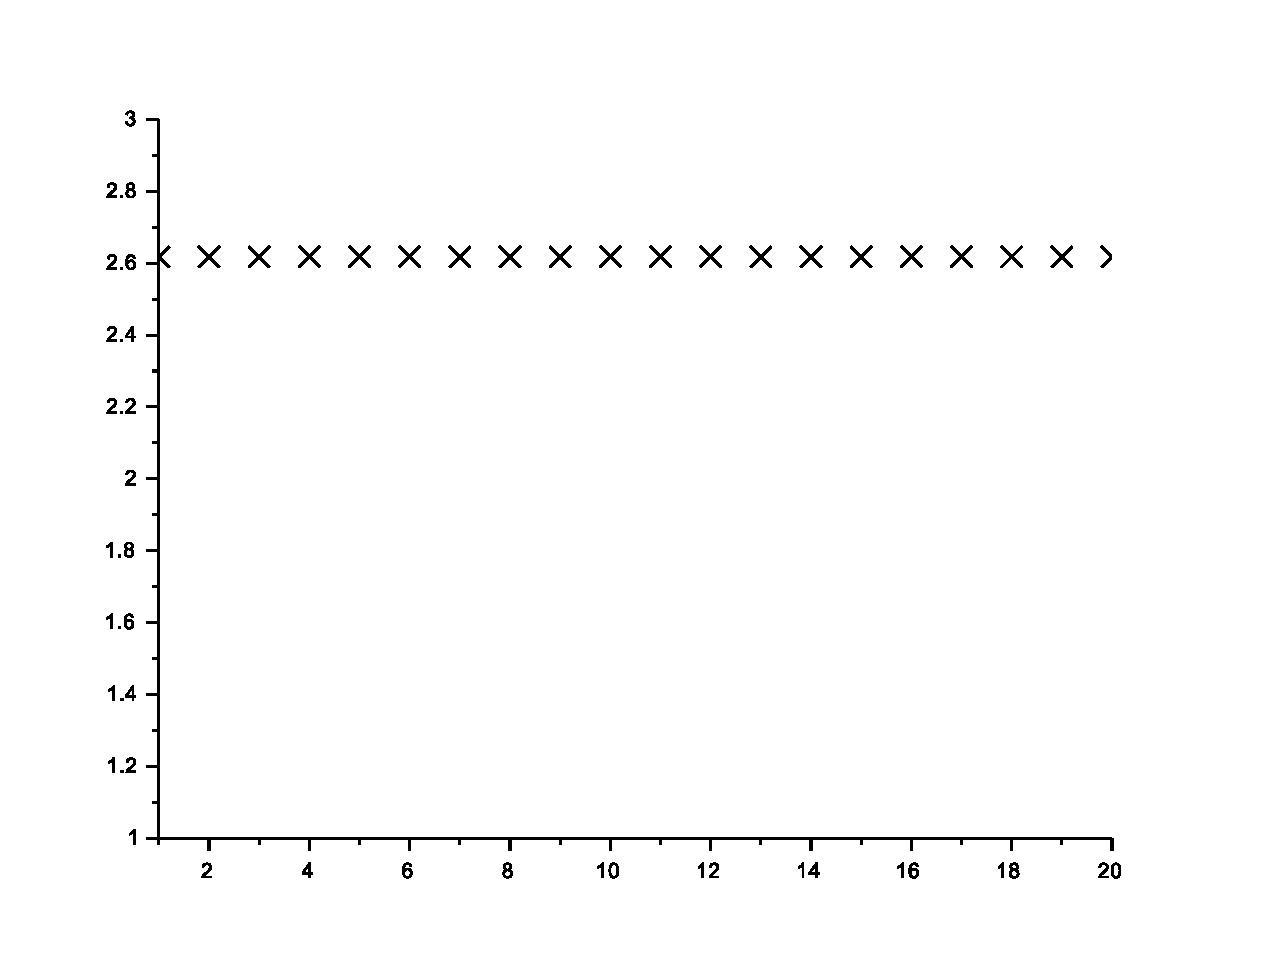
\includegraphics[width=9.5cm,height=9.5cm]{../Figures/ECRICOME_2019/Ecricome_2019_figure2.pdf}
    \end{center}
    Expliquer ce qui est affiché sur le graphique ci-dessus.\\
    Que peut-on conjecturer ?
    

    \newpage


    \begin{proof}~%
      \begin{noliste}{$\sbullet$}
      \item Le programme commence par définir deux tableaux (matrices
        lignes) {\tt X} et {\tt Y}.\\[-.3cm]
        \begin{scilab}
          & X = 1:20 \nl %
          & Y = zeros(1,20) \nl %
        \end{scilab}
        Le tableau {\tt X} contient initialement $[1, 2, \ldots,
        20]$, c'est-à-dire les $20$ premiers entiers non nuls.\\
        Le tableau {\tt Y} est destiné à contenir les $20$ premières
        valeurs de la suite $(v_n{}^n)$.\\
        Il est initialement rempli de $0$.

       \item À l'aide d'une boucle, la $\eme{k}$ case {\tt Y} est
         modifiée de sorte à contenir une valeur approchée de
         $v_k^k$.\\[-.3cm] 
        \begin{scilabC}{2}
          & \tcFor{for} k = 1:20 \nl %
          & \quad Y(k) = v(k)\puis{}k \nl %
          & \tcFor{end} 
        \end{scilabC}

      \item On effectue alors le tracé des points d'abscisse une
        valeur de {\tt X} et d'ordonnée la valeur correspondante de
        {\tt Y}. On obtient ainsi le tracé des points de coordonnées
        $(k, v_k^k)$ pour $k$ variant de $1$ à $20$.\\[-.3cm]
        \begin{scilabC}{5}
          & plot2d(X, Y, style=-2, rect=[1,1,20,3])
        \end{scilabC}
      \end{noliste}
      \concL{Le nuage de points obtenu correspond au tracé des $20$
        premières valeurs de la suite $(v_n{}^n)$.\\
        Au vu de la représentation graphique obtenue, on peut faire la
        conjecture que la suite $(v_n{}^n)$ est constante et
        approximativement de valeur $2.61$.}{15.4}~\\[-1cm]
    \end{proof}

  \item Montrer : $\forall n \geq 1, \ (v_n)^n = \dfrac{3+
      \sqrt{5}}{2}$.
    
    \begin{proof}~\\%
      Soit $n \in \N^*$.
      \begin{noliste}{$\sbullet$}
      \item Par définition de la suite $(v_n)$ : $h_n(v_n) = 4$. Ainsi
        :
        \[
        (v_n)^n + 1 + \dfrac{1}{(v_n)^n} = 4 \quad \text{ ou encore }
        \quad (v_n)^n - 3 + \dfrac{1}{(v_n)^n} = 0
        \]
        En multipliant par $(v_n)^n$, on obtient alors : 
        \[
        \big( (v_n)^n \big)^2 - 3 \, (v_n)^n + 1 = 0
        \]
        \conc{Ainsi, $(v_n)^n$ apparaît comme racine du polynôme $P(X)
          = X^2 - 3 \, X + 1$.}~

      \item Le polynôme $P$ admet pour discriminant : $\Delta = 9 - 4
        = 5 > 0$.\\
        Il admet donc deux racines réelles distinctes :
        \[
        x_+ = \dfrac{3 + \sqrt{5}}{2} \quad \text{ et } \quad x_- =
        \dfrac{3 - \sqrt{5}}{2}
        \]
        Comme $4 < 5 < 9$, on a : $\sqrt{4} < \sqrt{5} < \sqrt{9}$ \
        et \ $-2 > - \sqrt{5} > -3$. On en déduit :
        \[
        \dfrac{5}{2} \ < \ \dfrac{3 + \sqrt{5}}{2} \ < \ 3 \quad
        \text{ et } \quad 0 \ < \ \dfrac{3 - \sqrt{5}}{2} \ < \
        \dfrac{1}{2}
        \]


        \newpage


      \item Or, comme $v_n > 1$, par stricte croissance de la fonction
        $x \mapsto x^n$ sur $]1, +\infty[$, on a : 
        \[
        (v_n)^n \ > \ 1^n = 1
        \]
        On en déduit : $(v_n)^n \neq x_-$. %
      \end{noliste}
      \conc{Ainsi, pour tout $n \in \N^*$, $(v_n)^n = \dfrac{3 +
          \sqrt{5}}{2}$.}%
      \begin{remark}
        Dans cette question, on démontre la propriété :
        $\dfrac{3+\sqrt{5}}{2} \in \ ]2.5, 3[$.\\
        En prenant $2.24$ comme valeur approchée de $\sqrt{5}$, on
        obtient alors la valeur approchée :
        \[
        \dfrac{3 + \sqrt{5}}{2} \ \simeq \ 2.62
        \]
        Cela correspond à la valeur affichée par le graphique de la
        question \itbf{6.d)}.
      \end{remark}~\\[-1.2cm]
    \end{proof}

  \item Retrouver ainsi le résultat de la question \itbf{6.c)}.

    \begin{proof}~\\%
      Soit $n \in \N^*$.
      \begin{noliste}{$\sbullet$}
      \item D'après la question précédente : $(v_n)^n = \dfrac{3 +
          \sqrt{5}}{2}$. Comme $v_n > 0$, on en déduit :
        \[
        n \, \ln(v_n) \ = \ \ln\left( \dfrac{3 + \sqrt{5}}{2} \right)
        \quad \text{ ou encore } \quad \ln(v_n) \ = \ \dfrac{1}{n} \
        \ln\left( \dfrac{3 + \sqrt{5}}{2} \right)
        \]

      \item Finalement :
        \[
        v_n \ = \ \exp\big( \ln(v_n) \big) \ = \ \exp \left(
          \dfrac{1}{n} \ \ln\left( \dfrac{3 + \sqrt{5}}{2} \right)
        \right) \ \tendn \ \exp(0) \ = \ 1
        \]        
      \end{noliste}
      \conc{On retrouve le résultat de la question \itbf{6.c)} : la
        suite $(v_n)$ converge vers $1$.}~\\[-1.2cm]
    \end{proof}
  \end{noliste}
\end{noliste}


\newpage


\section*{Exercice 3}
\noindent
On suppose que toutes les variables aléatoires présentées dans cet exercice 
sont définies sur le même espace probabilisé.

\subsection*{Partie A} 
\noindent
Soit $f$ la fonction définie sur $\R$ par :
\[
  \forall t \in \R, \ f(t)= \left\{
  \begin{array}{cR{2.5cm}}
    \dfrac{1}{t^3} & si $t \geq 1$
    \nl
    \nl[-.2cm]
    0 & si $-1 < t < 1$
    \nl
    \nl[-.2cm]
    -\dfrac{1}{t^3} & si $t \leq -1$
  \end{array}
  \right.
\]
\begin{noliste}{1.}
  \setlength{\itemsep}{4mm}
  \item Démontrer que la fonction $f$ est paire.
  
    \begin{proof}~\\
      Soit $t \in \R$, alors : $-t \in \R$.\\
      Trois cas se présentent.
    \begin{noliste}{$\sbullet$}
    \item \dashuline{Si $t \in \ ]-\infty, -1]$}, alors $-t \in [1,
      +\infty[$. Donc :
      \[
        f(-t) \ = \ \dfrac{1}{(-t)^3} \ = \ \dfrac{1}{-t^3} \ = \ -
        \dfrac{1}{t^3} \ = \ f(t)
      \]

    \item \dashuline{Si $t \in \ ]-1,1[$}, alors $-t \in \
      ]-1,1[$. Donc :
      \[
        f(-t) \ = \ 0 \ = \ f(t)
      \]

    \item \dashuline{Si $t \in [1,+\infty[$}, alors $-t \in \
      ]-\infty, -1]$. Donc :
      \[
        f(-t) \ = \ - \dfrac{1}{(-t)^3} \ = \ -\dfrac{1}{-t^3} \ = \
        \dfrac{1}{t^3} \ = \ f(t)
      \]
    \end{noliste}
    Finalement, pour tout $t \in \R$ : $f(-t) = f(t)$.
    \conc{On en déduit que la fonction $f$ est paire.}~\\[-1cm]
  \end{proof}

  
  \item Justifier que l'intégrale $\dint{1}{+\infty} f(t) \dt$ converge et 
    calculer sa valeur.

    \begin{proof}~
      \begin{noliste}{$\sbullet$}
      \item La fonction $f$ est continue par morceaux sur $[1,+\infty[$.
        
      \item Soit $A \in [1,+\infty[$.
        \[
          \dint{1}{A} f(t) \dt \ = \ \dint{1}{A} \dfrac{1}{t^3} \dt \ =
          \ \dint{1}{A} t^{-3} \dt \ = \ \Prim{\dfrac{1}{-2} \
            t^{-2}}{1}{A} \ = \ -\dfrac{1}{2}\left( \dfrac{1}{A^2} - 1
          \right) \ = \ -\dfrac{1}{2 \, A^2} + \dfrac{1}{2}
        \]
        Or : $\dlim{A\to + \infty} \dfrac{1}{2 \, A^2} \ = \ 0$.
        \conc{Ainsi l'intégrale $\dint{1}{+\infty} f(t) \dt$ converge
          et vaut $\dfrac{1}{2}$.}~\\[-1.4cm]
      \end{noliste}
    \end{proof}


    \newpage
    
  
  \item
  \begin{noliste}{a)}
    \setlength{\itemsep}{2mm}
    \item \`A l'aide d'un changement de variable, montrer que pour
      tout réel $A$ strictement supérieur à 1, on a :
    \[
      \dint{-A}{-1} f(t) \dt \ = \ \dint{1}{A} f(u) \ du
    \]
    En déduire que l'intégrale $\dint{-\infty}{-1} f(t) \dt$ converge et donner sa valeur.

    \begin{proof}~
      \begin{noliste}{$\sbullet$}
      \item Soit $A \in \ ]1, +\infty[$.
      \end{noliste}
        \begin{liste}{$\stimes$}
        \item La fonction $f$ est continue par morceaux sur $[-A, -1]$.\\
          Ainsi, l'intégrale $\dint{-A}{-1} f(t)  \dt$ est bien définie.

        \item On effectue le changement de variable $\Boxed{u = - t}$.
          \[
            \left|
              \begin{array}{P{6cm}}
                $u = - t$ \quad (et donc $t = - u$) \nl
                $\hookrightarrow$ $du = -dt$ \quad et \quad $dt = -du$
                \nl
                \vspace{-.4cm}
                \begin{noliste}{$\sbullet$}
                \item $t = -A \ \Rightarrow \ u = A$
                \item $t = -1 \ \Rightarrow \ u = 1$ % \vspace{-.4cm}
                \end{noliste}
              \end{array}
            \right. %
          \]
          Ce changement de variable est valide car $\varphi : u
          \mapsto - u$ est de classe $\Cont{1}$ sur $[-A,-1]$.
        \item On obtient alors :
          \[
            \begin{array}{rcl@{\quad}>{\it}R{5cm}}
              \dint{-A}{-1} f(t) \dt
              & = & \dint{A}{1} f(-u) \big(- \ du\big)
              \\[.6cm]
              & = & \dint{1}{A} f(-u) \ du
              \\[.6cm]
              & = & \dint{1}{A} f(u) \ du
              & (car $f$ est paire d'après \itbf{1.})
            \end{array}
          \]
          \conc{Pour tout $A \in \ ]1,+\infty[$ : $\dint{-A}{-1} f(t)
            \dt = \dint{1}{A} f(u) \ du$.}
        \end{liste}
      \begin{noliste}{$\sbullet$}
      \item D'après la question précédente, l'intégrale
        $\dint{1}{+\infty} f(t) \dt$  converge.\\
        On déduit alors de l'égalité du point précédent que
        l'intégrale  $\dint{-\infty}{-1} f(t) \dt$ converge et, en
        passant à la limite quand $A$ tend vers $+\infty$, on obtient :
        \[
          \dint{-\infty}{-1} f(t) \dt \ = \ \dint{1}{+\infty} f(t) \dt
          \ = \ \dfrac{1}{2}
        \]
        \conc{L'intégrale $\dint{-\infty}{-1} f(t) \dt$ converge et
          vaut $\dfrac{1}{2}$.}~\\[-1.4cm]
      \end{noliste}
    \end{proof}


    \newpage
    

  \item Montrer que la fonction $f$ est une densité de probabilité.

    \begin{proof}~
      \begin{noliste}{$\sbullet$}
      \item La fonction $f$ est continue : \\[-.6cm]
      \end{noliste}
      \begin{liste}{$\stimes$}
      \item sur $]-\infty, -1[$, en tant qu'inverse de la fonction $t
        \mapsto t^3$ :
        \begin{noliste}{$-$}
        \item continue sur $]-\infty, -1[$ car polynomiale,
        \item et qui ne s'annule pas sur $]-\infty, -1[$.
        \end{noliste}
          
      \item sur $]-1,1[$, en tant que fonction constante,
          
      \item sur $]1,+\infty[$, en tant qu'inverse de la fonction $t
        \mapsto -t^3$ continue (car polynomiale) et qui ne s'annule
        pas sur cet intervalle.
      \end{liste}
      \conc{On en déduit que la fonction $f$ est continue sur $\R$
        sauf éventuellement en $-1$ et en $1$.}
        
      \begin{noliste}{$\sbullet$}
      \item Soit $t \in \R$. Trois cas se présentent :
        \begin{noliste}{$\stimes$}
        \item \dashuline{si $t \in \ ]-\infty, -1]$}, alors en
          particulier : $t < 0$. Donc : $t^3 < 0$. Ainsi :
          $\dfrac{1}{t^3} <0$.\\
          D'où : $f(t) = - \dfrac{1}{t^3} >0$.
          
        \item \dashuline{si $t \in \ ]-1,1[$}, alors : $f(t) =
          0$. Ainsi : $f(t) \geq 0$.
          
        \item \dashuline{si $t \in [1,+\infty[$}, alors en particulier
          : $t>0$. Ainsi : $f(t) = \dfrac{1}{t^3} >0$.
        \end{noliste}
        \conc{Finalement : $\forall t \in \R$, $f(t) \geq 0$.}
        
      \item Montrons que l'intégrale $\dint{-\infty}{+\infty} f(t)
        \dt$ converge et vaut $1$.
        \begin{noliste}{$\stimes$}
        \item D'après la question \itbf{3.a)}, l'intégrale
          $\dint{-\infty}{-1} f(t) \dt$ converge et vaut
          $\dfrac{1}{2}$.
          
        \item La fonction $f$ est nulle sur $]-1,1[$, donc
          l'intégrale $\dint{-1}{1} f(t) \dt$ converge
          et vaut $0$.
          
        \item D'après la question \itbf{2.}, l'intégrale
          $\dint{1}{+\infty} f(t) \dt$ converge et vaut
          $\dfrac{1}{2}$.
          
        \item On en déduit que l'intégrale $\dint{-\infty}{+\infty}
          f(t) \dt$ converge et :
          \[
            \dint{-\infty}{+\infty} f(t) \dt \ = \ \dint{-\infty}{-1}
            f(t) \dt + \dint{-1}{1} f(t) \dt + \dint{1}{+\infty} f(t)
            \dt \ = \ \dfrac{1}{2} + 0 + \dfrac{1}{2} \ = \ 1
          \]
        \end{noliste}
        \conc{L'intégrale $\dint{-\infty}{+\infty} f(t) \dt$ converge
          et vaut $1$.}
      \end{noliste}
      \conc{On en déduit que la fonction $f$ est une densité de
        probabilité.}~\\[-1.2cm]  
    \end{proof}
  \end{noliste}

  
  % \newpage
  
  
\item On considère une variable aléatoire $X$ admettant $f$ pour
  densité. On note $F_X$ la fonction de répartition de $X$.
  \begin{noliste}{a)}
    \setlength{\itemsep}{2mm}
  \item Montrer que, pour tout réel $x$, on a :
    \[
    F_X(x) \ = \ \left\{
      \begin{array}{cR{2.5cm}}
        \dfrac{1}{2x^2} & si $x \leq -1$
        \nl
        \nl[-.2cm]
        \dfrac{1}{2} & si $-1 < x < 1$
        \nl
        \nl[-.2cm]
        1 - \dfrac{1}{2 x^2} & si $x \geq 1$
      \end{array}
    \right.
    \]
    
    
    \newpage
    
    
    \begin{proof}~\\
      Soit $x \in \R$. Trois cas se présentent.
      \begin{noliste}{$\sbullet$}
      \item \dashuline{Si $x \in \ ]-\infty, -1]$}, alors :
        \[
        F_X(x) \ = \ \Prob(\Ev{X \leq x}) \ = \ \dint{-\infty}{x} f(t) \dt
        \]
        Soit $A \in \ ]-\infty, x]$. On a :
        \[
        \dint{A}{x} f(t) \dt \ = \ \dint{A}{x} - \dfrac{1}{t^3} \dt \
        = \ - \Prim{\dfrac{1}{-2} \ \dfrac{1}{t^2}}{A}{x} \ = \
        \dfrac{1}{2}\left( \dfrac{1}{x^2} - \dfrac{1}{A^2}\right) \ =
        \ \dfrac{1}{2 \, x^2} - \dfrac{1}{2 \, A^2}
        \]
        De plus : $\dlim{A \to - \infty} \dfrac{1}{2 \, A^2} = 0$.\\
        On en déduit : $F_X(x) \ = \ \dfrac{1}{2 \, x^2}$.
        
      \item \dashuline{Si $x \in \ ]-1,1[$}, alors :
        \[
        \begin{array}{rcl@{\qquad}>{\it}R{5cm}}
          F_X(x)
          & = & \dint{-\infty}{x} f(t) \dt
          \\[.6cm]
          & = & \dint{-\infty}{-1} f(t) \dt
          & (car $f$ est nulle en dehors de $]-\infty, -1] \cup
          [1,+\infty[$)
          \nl
          \nl[-.2cm]
          & = & \dfrac{1}{2}
        \end{array}
        \]
        
      \item \dashuline{Si $x \in [1,+\infty[$}, alors :
        \[
        \begin{array}{rcl@{\quad}>{\it}R{5cm}}
          F_X(x)
          & = & \dint{-\infty}{x} f(t) \dt
          \\[.6cm]
          & = & \dint{-\infty}{-1} f(t) \dt + \dint{-1}{1} f(t) \dt
          + \dint{1}{x} f(t) \dt
          \\[.6cm]
          & = & \dfrac{1}{2} + 0 + \dint{1}{x} \dfrac{1}{t^3} \dt
          & (car $f$ est nulle en dehors de $]-\infty, -1] \cup
          [1,+\infty[$)
          \nl
          \nl[-.2cm]
          & = & \dfrac{1}{2} + \Prim{\dfrac{1}{-2} \
            \dfrac{1}{t^2}}{1}{x}
          \\[.6cm]
          & = & \dfrac{1}{2} - \dfrac{1}{2}\left(\dfrac{1}{x^2} -
            1\right)
          \\[.6cm]
          & = & \dfrac{1}{2} - \dfrac{1}{2 \, x^2} + \dfrac{1}{2}
        \end{array}
        \]
      \end{noliste}
      \conc{Finalement : $F_X : x \mapsto \left\{
          \begin{array}{cR{2.5cm}}
            \dfrac{1}{2 \, x^2} & si $x \leq -1$
            \nl
            \nl[-.2cm]
            \dfrac{1}{2} & si $-1 < x < 1$
            \nl
            \nl[-.2cm]
            1- \dfrac{1}{2 \, x^2} & si $x \geq 1$               
          \end{array}
        \right.$.}~\\[-1.2cm]
    \end{proof}
    
    \newpage
    
  \item Démontrer que $X$ admet une espérance, puis que cette
    espérance est nulle.
    
    \begin{proof}~
      \begin{noliste}{$\sbullet$}
      \item La \var $X$ admet une espérance si et seulement si
        l'intégrale $\dint{-\infty}{+\infty} t \, f(t) \dt$ est
        absolument convergente, ce qui équivaut à démontrer la
        convergence pour ce calcul de moment du type
        $\dint{-\infty}{+\infty} t^m \, f(t) \dt$.
          
      \item Commençons par étudier la convergence de l'intégrale
        $\dint{0}{+\infty} t \, f(t) \dt$.
        \begin{noliste}{$\stimes$}
        \item Tout d'abord, comme la fonction $f$ est nulle en
          dehors de $]-\infty, -1] \cup [1,+\infty[$ :
          \[
          \dint{0}{+\infty} t \, f(t) \dt \ = \ \dint{1}{+\infty}
          t \, f(t) \dt
          \]
          
        \item De plus, la fonction $t \mapsto t \, f(t)$ est
          continue par morceaux sur $[1,+\infty[$.
          
        \item Enfin, soit $t \in [1,+\infty[$ :
          \[
          t \, f(t) \ = \ t \ \dfrac{1}{t^3} \ = \ \dfrac{1}{t^2}
          \]
          Or, l'intégrale $\dint{1}{+\infty} \dfrac{1}{t^2} \dt$ est
          une intégrale de Riemann, impropre en $+\infty$,
          d'exposant $2 > 1$. Elle est donc convergente.
        \end{noliste}
        \conc{On en déduit que l'intégrale $\dint{0}{+\infty} t \, f(t)
          \dt$ converge.}
        
      \item D'après la question \itbf{1.}, la fonction $f$ est
        paire.\\
        On en déduit que la fonction $t \mapsto t \, f(t)$ est
        impaire.%
        \conc{Ainsi, l'intégrale $\dint{-\infty}{0} t \, f(t) \dt$
          converge et : $\dint{-\infty}{0} t \, f(t) \dt = -
          \dint{0}{+\infty} f(t) \dt$.}
        
      \item On en déduit que l'intégrale $\dint{-\infty}{+\infty} t
        \, f(t) \dt$ converge. %
        \conc{Ainsi, la \var $X$ admet une espérance.}
        
      \item Enfin :
        \[
        \begin{array}{rcl}
          \E(X) & = & \dint{-\infty}{+\infty} t \, f(t) \dt 
          \\[.8cm]
          & = &
          \dint{-\infty}{0} t \, f(t) \dt + \dint{0}{+\infty} t \,
          f(t) \dt 
          \\[.8cm]
          & = &
          -\dint{0}{+\infty} t \, f(t) \dt +
          \dint{0}{+\infty} t \, f(t) \dt \ = \ 0
        \end{array}
        \]
        \conc{$\E(X) = 0$}
      \end{noliste}
      \begin{remark}
        On rappelle que l'égalité :
        \[
        \dint{-\infty}{0} t \, f(t) \dt \ = \ - \dint{0}{+\infty} t
        \, f(t) \dt
        \]
        se démontre à l'aide du changement de variable $\Boxed{u =
          -t}$.
        \[
        \left|
          \begin{array}{P{6cm}}
            $u = - t$ \quad (et donc $t = - u$) \nl
            $\hookrightarrow$ $du = -dt$ \quad et \quad $dt = -du$
            \nl
            \vspace{-.2cm}
            \begin{noliste}{$\sbullet$}
            \item $t = -\infty \ \Rightarrow \ u = +\infty$
            \item $t = 0 \ \Rightarrow \ u =0$ % \vspace{-.4cm}
            \end{noliste}
          \end{array}
        \right. %
        \]
        Ce changement de variable est valide car $\varphi : u
        \mapsto - u$ est de classe $\Cont{1}$ sur $]-\infty,0]$.
      \end{remark}~\\[-1.4cm]
    \end{proof}
    
  \item La variable aléatoire $X$ admet-elle une variance ?
    
    \begin{proof}~
      \begin{noliste}{$\sbullet$}
      \item La \var $X$ admet une variance si et seulement si
        l'intégrale $\dint{-\infty}{+\infty} t^2 \, f(t) \dt$ est
        absolument convergent, ce qui équivaut à démontrer la
        convergence pour ce calcul de moment du type
        $\dint{-\infty}{+\infty} t^m \, f(t) \dt$.
        
        
        % \newpage
        
        
      \item Commençons par étudier la nature de l'intégrale
        $\dint{0}{+\infty} t^2 \, f(t) \dt$.
        \begin{noliste}{$\stimes$}
        \item Tout d'abord, comme la fonction $f$ est nulle en
          dehors de $]-\infty, -1] \cup [1,+\infty[$ :
          \[
          \dint{0}{+\infty} t^2 \, f(t) \dt \ = \ \dint{1}{+\infty}
          t^2 \, f(t) \dt
          \]
          
        \item De plus, la fonction $t \mapsto t^2 \, f(t)$ est
          continue par morceaux sur $[1,+\infty[$.
          
        \item Enfin, soit $t \in [1,+\infty[$ :
          \[
          t^2 \, f(t) \ = \ t^2 \ \dfrac{1}{t^3} \ = \ \dfrac{1}{t}
          \]
          Or, l'intégrale $\dint{1}{+\infty} \dfrac{1}{t} \dt$ est
          une intégrale de Riemann, impropre en $+\infty$,
          d'exposant $1$. Elle est donc divergente.
        \end{noliste}
        \conc{On en déduit que l'intégrale $\dint{0}{+\infty} t^2 \,
          f(t) \dt$ diverge.}
        
      \item Ainsi, l'intégrale $\dint{-\infty}{+\infty} t^2 f(t)
        \dt$ diverge.%
        \conc{On en déduit que la \var $X$ n'admet pas de
          variance.}
      \end{noliste}
      \begin{remark}
        Lorsqu'un résultat à démontrer est formulé sous forme
        d'interrogation (et pas d'affirmation comme c'est le cas en
        général), on pensera, dans une majorité de cas à répondre
        par la négative. À titre d'illustration, lorqu'on rencontre
        les questions :
        \begin{noliste}{$\stimes$}
        \item \og Les \var $X$ et $Y$ sont-elles indépendantes ?
          \fg{}
          
        \item \og La \var $X$ admet-elle une variance ? \fg{}
          
        \item \og La matrice $A$ est-elle diagonalisable ? \fg{}
          
        \item \og La suite $(u_n)$ est-elle majorée ? \fg{}
        \end{noliste}
        la réponse est, généralement, \og non \fg{} (à justifier
        évidemment).
      \end{remark}~\\[-1.4cm]
    \end{proof}
  \end{noliste}
  
\item Soit $Y$ la variable aléatoire définie par $Y=|X|$.
  \begin{noliste}{a)}
    \setlength{\itemsep}{2mm}
  \item Donner la fonction de répartition de $Y$, et montrer que $Y$
    est une variable aléatoire à densité.

    \begin{proof}~
      \begin{noliste}{$\sbullet$}
      \item Tout d'abord, par définition de $Y$ : $Y(\Omega) \subset
        [0, +\infty[$.
        
      \item Soit $x \in \R$. Deux cas se présentent :
        \begin{noliste}{$\stimes$}
        \item \dashuline{si $x \in \ ]-\infty, 0[$}, alors $\Ev{Y
            \leq x} = \emptyset$, car $Y(\Omega) \subset
          [0,+\infty[$. Donc :
          \[
          F_Y(x) \ = \ \Prob(\Ev{Y \leq x}) \ = \
          \Prob(\emptyset) \ = \ 0
          \]
          
        \item \dashuline{si $x \in [0,+\infty[$}, alors :
          \[
          F_Y(x) \ = \ \Prob(\Ev{Y \leq x}) \ = \ \Prob(\Ev{|X|
            \leq x}) \ = \ \Prob(\Ev{ -x \leq X \leq x}) \ = \
          F_X(x) - F_X(-x)
          \]
          où la dernière égalité est obtenue car $X$ est une \var à
          densité.\\
          Deux cas se présentent alors :
        \end{noliste}
        \begin{liste}{-}
        \item \underline{si $x \in [0,1[$}, alors $-x \in \ ]-1,0]$.
          On obtient alors avec la question \itbf{4.a)} :
          \[
          F_Y(x) \ = \ F_X(x) - F_x(-x) \ = \ \bcancel{\dfrac{1}{2}} -
          \bcancel{\dfrac{1}{2}} \ = \ 0
          \]

        \item \underline{si $x \in [1,+\infty[$}, alors $-x \in \
          ]-\infty, -1]$.  On obtient alors avec la question
          \itbf{4.a)} :
          \[
          F_Y(x) \ = \ F_X(x) - F_X(-x) \ = \ \left(1- \dfrac{1}{2 \,
              x^2}\right) - \dfrac{1}{2 \, (-x)^2} \ = \ 1 -
          \dfrac{1}{2 \, x^2} - \dfrac{1}{2 \, x^2} \ = \ 1-
          \dfrac{1}{x^2}
          \]
        \end{liste}
        \conc{Finalement : $F_Y : x \mapsto \left\{
            \begin{array}{cR{2.5cm}}
              0 & si $x \in \ ]-\infty, 1[$
              \nl
              \nl[-.2cm]
              1-\dfrac{1}{x^2} & si $x \in [1,+\infty[$
            \end{array}
          \right.$.}
        
        
        \newpage
        
        
      \item Montrons que $Y$ est une \var à densité.
      \end{noliste}
      \begin{liste}{$\stimes$}
      \item La fonction $F_Y$ est continue :
        \begin{noliste}{-}
        \item sur $]-\infty, 1[$, en tant que fonction constante,
          
        \item sur $]1,+\infty[$, en tant que somme de fonctions
          continues sur $]1,+\infty[$,
          
        \item en $1$. En effet, d'une part : $\dlim{x\to 1^+} F_Y(x)
          \ = \ F_Y(1) \ = \ 1- \dfrac{1}{1^2} \ = \ 0$.\\
          D'autre part : $\dlim{x \to 1^-} F_Y(x) = 0$. Ainsi :
          \[
          \dlim{x \to 1^-} F_Y(x) \ = \ F_Y(1) \ = \ \dlim{x\to
            1^+} F_Y(x)
          \]
        \end{noliste}
        \conc{La fonction $F_Y$ est continue sur $\R$.}
        
      \item La fonction $F_Y$ est de classe $\Cont{1}$ sur $]-\infty,
        1[$ et $]1, +\infty[$ avec des arguments similaires à ceux de
        la continuité sur ces intervalles.
        \conc{La fonction $F_Y$ est de classe $\Cont{1}$ sur $\R$
          sauf éventuellement en $1$.}
      \end{liste}
      \conc{On en déduit que la \var $Y$ est une \var à densité.}~\\[-1cm]
    \end{proof}
    
  \item Montrer que $Y$ admet pour densité la fonction $f_Y$ définie
    par :
    \[
    f_Y : x \mapsto \left\{
      \begin{array}{cR{2cm}}
        \dfrac{2}{x^3} & si $x \geq 1$
        \nl
        \nl[-.2cm]
        0 & sinon 
      \end{array}
    \right. 
    \]
    
    \begin{proof}~\\
      Pour déterminer une densité $f_Y$ de $Y$, on dérive la fonction
      $F_Y$ sur les intervalles {\bf ouverts} $]-\infty, 1[$ et
      $]1,+\infty[$. Soit $x \in \R$.
      \begin{noliste}{$\sbullet$}
      \item \dashuline{Si $x \in \ ]-\infty, 1[$}.
        \[
        f_Y(x) \ = \ F_Y'(x) \ = \ 0
        \]
        
      \item \dashuline{Si $x \in \ ]1, +\infty[$}.
        \[
        f_Y(x) \ = \ F_Y'(x) \ = \ -(-2) \ \dfrac{1}{x^3} \ = \ \dfrac{2}{x^3}
        \]
        
      \item On choisit enfin : $f_Y(1) =
        \dfrac{2}{1^3} = 2$.
      \end{noliste}
      \conc{Ainsi, une densité $f_Y$ de $Y$ est : $f_Y : x \mapsto
        \left\{
          \begin{array}{cR{2.5cm}}
            0 & si $x \in \ ]-\infty, 1[$
            \nl
            \nl[-.2cm]
            \dfrac{2}{x^3} & si $x \in [1,+\infty[$
          \end{array}
        \right.$.}~\\[-1cm]
    \end{proof}
    
  \item Montrer que $Y$ admet une espérance et la calculer.
    \begin{proof}~
      \begin{noliste}{$\sbullet$}
      \item La \var $Y$ admet une espérance si et seulement si
        l'intégrale $\dint{-\infty}{+\infty} t \, f_Y(t) \dt$ est
        absolument convergente, ce qui équivaut à démontrer la
        convergence pour ce calcul de moment du type
        $\dint{-\infty}{+\infty} t^m \, f_Y(t) \dt$.
          
      \item Tout d'abord, comme la fonction $f_Y$ est nulle en dehors
        de $[1,+\infty[$ :
        \[
        \dint{-\infty}{+\infty} t \, f_Y(t) \dt \ = \
        \dint{1}{+\infty} t \, f_Y(t) \dt
        \]
            
      \item De plus, la fonction $t \mapsto t \, f_Y(t)$ est continue
        par morceaux sur $[1,+\infty[$.
            
      \item Enfin, soit $t \in [1,+\infty[$ :
        \[
        t \, f_Y(t) \ = \ t \ \dfrac{3}{t^3} \ = \ \dfrac{2}{t^2}
        \]
        Ainsi, soit $B \in [1, +\infty[$.
        \[
        \dint{1}{B} t \, f_Y(t) \dt \ = \ \dint{1}{B} \dfrac{1}{t^2}
        \dt \ = \ 2 \ \dint{1}{B} t^{-2} \dt \ = \ \bcancel{2} \
        \Prim{\dfrac{1}{-\bcancel{2}} \ t^{-1}}{1}{B} \ = \ -\left(
          \dfrac{1}{B} - 1\right) \ = \ 1 - \dfrac{1}{B}
        \]
        Or : $\dlim{B \to + \infty} \dfrac{1}{B} = 0$. On en déduit
        que l'intégrale $\dint{1}{+\infty} t \, f_Y(t) \dt$ converge.%
        \conc{Ainsi, la \var $Y$ admet une espérance.}
        
      \item De plus :
        \[
        \E(Y) \ = \ \dint{-\infty}{+\infty} t \, f_Y(t) \dt \ = \
        \dint{1}{+\infty} t \, f_Y(t) \dt \ = \ 1
        \]
        \conc{$\E(Y) = 1$}~\\[-1.4cm]
      \end{noliste}
    \end{proof}
  \end{noliste}
\end{noliste}

 
% \newpage


\subsection*{Partie B} 

\begin{noliste}{1.}
  \setlength{\itemsep}{4mm} %
  \setcounter{enumi}{5}
\item Soit $D$ une variable aléatoire prenant les valeurs $-1$ et $1$
  avec équiprobabilité, indépendante de la variable aléatoire $Y$.\\
  Soit $T$ la variable aléatoire définie par $T=DY$.
  \begin{noliste}{a)}
    \setlength{\itemsep}{2mm}
  \item Déterminer la loi de la variable $Z = \dfrac{D+1}{2}$. En
    déduire l'espérance et la variance de $D$.

    \begin{proof}~
      \begin{noliste}{$\sbullet$}
      \item D'après l'énoncé : $D \suit {\cal
          U}\left(\{-1,1\}\right)$. Ainsi :
        \begin{noliste}{$\stimes$}
        \item $D(\Omega) = \{-1,1\}$,
            
        \item $\Prob(\Ev{D = -1}) \ = \ \Prob(\Ev{ D = 1}) \ = \
          \dfrac{1}{2}$.
        \end{noliste}

      \item Tout d'abord, comme $D(\Omega) = \{-1, 1\}$, on obtient :
        $Z(\Omega) \ = \ \left\{ \dfrac{-1+1}{2},
          \dfrac{1+1}{2}\right\} \ = \ \{0,1\}$.
          
      \item De plus :
        \[
        \Ev{Z = 1} \ = \ \Ev{ \dfrac{D+1}{2} = 1} \ = \ \Ev{ D+1 =
          2} \ = \ \Ev{D = 1}
        \]
        On en déduit : $\Prob(\Ev{Z= 1}) \ = \ \Prob(\Ev{D = 1}) \ =
        \ \dfrac{1}{2}$.
      \end{noliste}
      \conc{Finalement : $Z \suit \Bern{\dfrac{1}{2}}$.}~\\[-1cm]
    \end{proof}
    
    
    \newpage
    
    
  \item Justifier que $T$ admet une espérance et préciser sa valeur.
    
    \begin{proof}~
      \begin{noliste}{$\sbullet$}
      \item La \var $T$ admet une espérance en tant que produit de
        \var indépendantes admettant une espérance. %
        \conc{La \var $T$ admet une espérance.}
          
      \item De plus :
        \[
        \begin{array}{rcl@{\quad}>{\it}R{5cm}}
          \E(T)
          & = & \E(DY)
          \\[.2cm]
          & = & \E(D) \ \E(Y)
          & (car $D$ et $Y$ sont indépendantes)  
        \end{array}
        \]
        
      \item Enfin, par définition de l'espérance :
        \[
        \E(D) \ = \ (-1) \times \Prob(\Ev{D = -1}) + 1 \times
        \Prob(\Ev{ D = 1}) \ = \ -\bcancel{\dfrac{1}{2}} +
        \bcancel{\dfrac{1}{2}} \ = \ 0
        \]
        \conc{On en déduit : $\E(T) = \E(D) \ \E(Y) = 0 \times \E(Y)
          = 0$.}~\\[-1.4cm]
      \end{noliste}
    \end{proof}
    
  \item Montrer que pour tout réel $x$, on a :
    \[
    \Prob(\Ev{T \leq x}) \ = \ \dfrac{1}{2} \ \Prob(\Ev{Y \leq x}) + 
    \dfrac{1}{2} \ \Prob(\Ev{Y \geq -x})
    \]
    
    \begin{proof}~\\
      Soit $x \in \R$.\\
      La famille $(\Ev{D = -1}, \Ev{D = 1})$ forme un système complet
      d'événements.\\
      Ainsi, par formule des probabilités totales :
      \[
      \begin{array}{rcl@{\qquad}>{\it}R{5cm}}
        \Prob(\Ev{T \leq x})
        & = & \Prob(\Ev{D = -1} \cap \Ev{T \leq x}) + \Prob(\Ev{D =
          1} \cap \Ev{T \leq x})
        \\[.2cm]
        & = & \Prob(\Ev{D = -1} \cap \Ev{DY \leq x}) + \Prob(\Ev{ D
          =1} \cap \Ev{DY \leq x})
        \\[.2cm]
        & = & \Prob(\Ev{D = -1} \cap \Ev{-Y \leq x}) + \Prob(\Ev{ D
          = 1} \cap \Ev{Y \leq x})
        \\[.2cm]
        & = & \Prob(\Ev{D = -1}) \ \Prob(\Ev{-Y \leq x}) +
        \Prob(\Ev{D = 1}) \ \Prob(\Ev{Y \leq x})
        & (car les \var $D$ et $Y$ \\ sont indépendantes)
        \nl
        \nl[-.2cm]
        & = & \dfrac{1}{2} \ \Prob(\Ev{Y \geq -x}) + \dfrac{1}{2} \
        \Prob(\Ev{Y \leq x})
      \end{array}
      \]
      \conc{$\forall x \in \R$, $\Prob(\Ev{T \leq x}) = \dfrac{1}{2} \
        \Prob(\Ev{Y \leq x}) + \dfrac{1}{2} \ \Prob(\Ev{Y \geq -x})$}~\\[-1cm]
    \end{proof}
    
  \item En déduire la fonction de répartition de $T$.
    
    \begin{proof}~\\
      Soit $x \in \R$.
      \begin{noliste}{$\sbullet$}
      \item D'après la question précédente :
        \[
        F_T(x) \ = \ \Prob(\Ev{T \leq x}) \ = \ \dfrac{1}{2} \
        \Prob(\Ev{Y \leq x}) + \dfrac{1}{2} \ \Prob(\Ev{Y \geq -x})
        \ = \ \dfrac{1}{2} \ F_Y(x) + \dfrac{1}{2} \left(1 - F_Y(-x)\right)
        \]
        où la dernière égalité est obtenue car $Y$ est une \var à
        densité d'après la question \itbf{5.a)}.
        

        \newpage


      \item Trois cas se présentent alors :
        \begin{noliste}{$\stimes$}
        \item \dashuline{si $x \in \ ]-\infty, -1]$}, alors $-x \in
          [1,+\infty[$. On obtient donc, avec la question \itbf{5.a)}
          :
          \[
          F_T(x) \ = \ \dfrac{1}{2} \times 0 + \dfrac{1}{2} \left(
            \bcancel{1} - \left(\bcancel{1}-
              \dfrac{1}{(-x)^2}\right)\right) \ = \ \dfrac{1}{2 \,
            x^2}
          \]
          
        \item \dashuline{si $x \in \ ]-1,1[$}, alors $-x \in \
          ]-1,1[$. On obtient donc, avec la question \itbf{5.a)} :
          \[
          F_T(x) \ = \ \dfrac{1}{2} \times 0 + \dfrac{1}{2}\left(1 -
            0\right) \ = \ \dfrac{1}{2}
          \]
          
        \item \dashuline{si $x \in [1,+\infty[$}, alors $-x \in \
          ]-\infty, -1]$. On obtient donc, avec la question
          \itbf{5.a)} :
          \[
          F_T(x) \ = \ \dfrac{1}{2}\left(1- \dfrac{1}{x^2}\right) +
          \dfrac{1}{2} \left(1 - 0\right) \ = \ \dfrac{1}{2} -
          \dfrac{1}{2 \, x^2} + \dfrac{1}{2} \ = \ 1 - \dfrac{1}{2 \,
            x^2}
          \]
        \end{noliste}
      \end{noliste}
      \conc{Finalement : $F_T : x \mapsto \left\{
          \begin{array}{cR{3.2cm}}
            \dfrac{1}{2 \, x^2} & si $x \in \ ]-\infty, -1]$
            \nl
            \nl[-.2cm]
            \dfrac{1}{2} & si $x \in \ ]-1,1[$
            \nl
            \nl[-.2cm]
            1 - \dfrac{1}{2 \, x^2} & si $x \in [1,+\infty[$               
          \end{array}
        \right.$.}
      \begin{remark}
        On remarque que les \var $T$ et $X$ ont même fonction de
        répartition. Or, la fonction de répartition caractérise la
        loi. On en déduit que les \var $X$ et $T$ ont même loi.
      \end{remark}~\\[-1.4cm]
    \end{proof}
  \end{noliste}
  
\item Soit $U$ une variable aléatoire suivant la loi uniforme sur $]0,1[$ 
  et $V$ la variable aléatoire définie par : $V = \dfrac{1}{\sqrt{1-U}}$.
  \begin{noliste}{a)}
    \setlength{\itemsep}{2mm}
  \item Rappeler la fonction de répartition de $U$.
    
    \begin{proof}~%
      \conc{Comme $U \suit \Uc{0}{1}$, alors $F_U : x \mapsto \left\{
          \begin{array}{cR{2.5cm}}
            0 & si $x \in \ ]-\infty, 0]$
            \nl
            \nl[-.2cm]
            x & si $x \in \ ]0,1[$
            \nl
            \nl[-.2cm]
            1 & si $x \in [1, +\infty[$        
          \end{array}
        \right.$.}~\\[-1cm]
    \end{proof}
    
  \item Déterminer la fonction de répartition de $V$ et vérifier que les 
    variable $V$ et $Y$ suivent la même loi.
    
    \begin{proof}~
      \begin{noliste}{$\sbullet$}
      \item On note $h : x \mapsto \dfrac{1}{\sqrt{1-x}}$ de telle
        sorte que $V = h(U)$.\\
        On sait tout d'abord : $U(\Omega) = \ ]0,1[$. On obtient alors
        :
        \[
        \begin{array}{rcl@{\quad}>{\it}R{6cm}}
          V(\Omega)
          & = & \big(h(U)\big)(\Omega) \ = \
          h\big(U(\Omega)\big)
          \\[.2cm]
          & = & h(]0,1[)
          \\[.2cm]
          & = & \left] \dlim{x\to 0} h(x), \dlim{x \to 1}
            h(x)\right[
          & (car $h$ est continue et \\ strictement croissante sur
          $]0,1[$) $(*)$
          \nl
          \nl[-.2cm]
          & = & ]1, +\infty[  
        \end{array}
        \]
        
        
        \newpage
          
          
        \noindent
        Détaillons $(*)$.
        \begin{noliste}{$\stimes$}
        \item La fonction $h$ est continue sur $]0,1[$ en tant que
          quotient de fonctions continues sur $]0,1[$ dont le
          dénominateur ne s'annule pas sur cet intervalle.
          
        \item La fonction $h$ est dérivable sur $]0,1[$ avec des
          arguments similaires.\\
          Soit $x \in \ ]0,1[$.
          \[
          h'(x) \ = \ - \dfrac{1}{2} \
          \dfrac{-1}{(1-x)^{\frac{3}{2}}} \ = \
          \dfrac{1}{2(1-x)^{\frac{3}{2}}} \ > \ 0
          \]
          Donc la fonction $h$ est bien strictement croissante sur $]0,1[$.
        \end{noliste}
        \conc{$V(\Omega) \ = \ ]1, +\infty|$}
        
      \item Soit $x \in \R$. Deux cas se présentent :
        \begin{noliste}{$\stimes$}
        \item \dashuline{si $x \in \ ]-\infty, 1]$}, alors : $\Ev{V
            \leq x} = \emptyset$, car $V(\Omega) = \
          ]1,+\infty[$. Donc :
          \[
          F_V(x) \ = \ \Prob(\Ev{V \leq x}) \ = \ \Prob(\emptyset) \
          = \ 0
          \]
          
        \item \dashuline{si $x \in \ ]1, +\infty[$}, alors :
          \[
          \begin{array}{rcl@{\quad}>{\it}R{6.5cm}}
            F_V(x)
            & = & \Prob(\Ev{V \leq x}) \ = \ \Prob\left(
              \Ev{ \dfrac{1}{\sqrt{1-U}} \leq x}\right)
            \\[.6cm]
            & = & \Prob\left( \Ev{\sqrt{1-U} \geq \dfrac{1}{x}}
            \right)
            & (car la fonction inverse est strictement
            décroissante sur $]0,+\infty[$)
            \nl
            \nl[-.2cm]
            & = & \Prob\left( \Ev{1-U \geq \dfrac{1}{x^2}} \right)
            & (car la fonction $x \mapsto x^2$ est strictement
            croissante sur $[0,+\infty[$)
            \nl
            \nl[-.2cm]
            & = & \Prob\left( \Ev{1-\dfrac{1}{x^2} \geq U}\right)
            \\[.6cm]
            & = & F_U\left(1 - \dfrac{1}{x^2}\right)
          \end{array}
          \]
          De plus :
          \[
          \begin{array}{R{2cm}C{1.8cm}l@{\qquad}>{\it}R{5cm}}
            & Comme & x > 1
            \\[.2cm]
            & alors & x^2 > 1
            & (par stricte croissance de la fonction $x
            \mapsto x^2$ sur $[0,+\infty[$)
            \nl
            \nl[-.2cm]
            & donc & \dfrac{1}{x^2} < 1
            & (par stricte décroissance de la fonction
            inverse sur $]0,+\infty[$)
            \nl
            \nl[-.2cm]
            & et & 0 < \dfrac{1}{x^2} < 1       
          \end{array}
          \]
          On en déduit, d'après la question précédente :
          \[
          F_V(x) \ = \ F_U\left(1 - \dfrac{1}{x^2} \right) \ = \ 1
          - \dfrac{1}{x^2}
          \]
        \end{noliste}
        \conc{Finalement : $F_V : x \mapsto \left\{
            \begin{array}{cR{2.5cm}}
              0 & si $x \in \ ]-\infty, 1]$
              \nl
              \nl[-.2cm]
              1 - \dfrac{1}{x^2} & si $x \in [1,+\infty[$    
            \end{array}
          \right.$.}
        
      \item On remarque que les \var $V$ et $Y$ ont même fonction de
        répartition, d'après la question \itbf{5.a)}. Or la fonction
        de répartition caractérise la loi.%
        \conc{On en déduit que les \var $V$ et $Y$ ont même loi.}~\\[-1.4cm]
      \end{noliste}
    \end{proof}
  \end{noliste}
  
    
  \newpage
    
  
\item
  \begin{noliste}{a)}
    \setlength{\itemsep}{2mm}
  \item Écrire une fonction en langage \Scilab{}, d'en-tête {\tt
      function a = D(n)}, qui prend un entier $n \geq 1$ en entrée, et
    renvoie une matrice ligne contenant $n$ réalisations de la
    variable aléatoire $D$.
    
    \begin{proof}~
      \begin{scilab}
        & \tcFun{function} \tcVar{a} = \underline{D}(\tcVar{n}) \nl %
        & \quad \tcVar{a} = zeros(1,\tcVar{n}) \nl %
        & \quad \tcFor{for} i = 1:\tcVar{n} \nl %
        & \quad \quad r = rand() \nl %
        & \quad \quad \tcIf{if} r < 1/2 \tcIf{then} \nl %
        & \quad \quad \quad \tcVar{a}(i) = -1 \nl %
        & \quad \quad \tcIf{else} \nl %
        & \quad \quad \quad \tcVar{a}(i) = 1 \nl %
        & \quad \quad \tcIf{end} \nl %
        & \quad \tcFor{end} \nl %
        & \tcFun{endfuntion}
      \end{scilab}
      
      \begin{noliste}{$\sbullet$}
      \item {\bf Début de la fonction}\\
        On commence par initialiser la variable {\tt a} qui doit
        contenir, d'après l'énoncé, une matrice ligne à {\tt n}
        colonnes.
        \begin{scilabC}{1}
          & \quad \tcVar{a} = zeros(1,\tcVar{n})
        \end{scilabC}
        
      \item {\bf Structure itérative}\\
        On met ensuite en place une structure itérative (boucle
        \tcFor{for}) pour affecter à chaque coefficient de la matrice
        {\tt a} une réalisation de la \var $D$.
        \begin{scilabC}{2}
          & \quad \tcFor{for} i = 1:\tcVar{n}
        \end{scilabC}
        On cherche maintenant à simuler la \var $D$.
        \begin{noliste}{$\stimes$}
        \item D'après l'énoncé : $D \suit {\cal U}(\{-1,1\})$.\\
          Ainsi, chaque coefficient de la variable {\tt a} doit :
        \end{noliste}
        \begin{liste}{-}
        \item prendre la valeur $-1$ avec probabilité $\Prob(\Ev{D=
            -1}) = \dfrac{1}{2}$.
          
        \item prendre la valeur $1$ avec probabilité $\Prob(\Ev{D =1})
          = \dfrac{1}{2}$.
        \end{liste}
        \begin{noliste}{$\stimes$}
        \item Pour cela, on utilise la commande suivante :
          \begin{scilabC}{4}
            & \quad \quad r = rand()
          \end{scilabC}
          L'instruction {\tt rand()} renvoie un réel choisi
          aléatoirement dans $]0,1[$.\\
          Plus formellement, il s'agit de simuler une \var $U$ telle
          que $U \suit \Uc{0}{1}$.
          
        \item  Cette valeur {\tt r} choisie aléatoirement dans $]0,1[$
          permet d'obtenir une simulation de $D$.
          \begin{center}
            %% French babel fout la merde : ne pas oublier shorthandoff
            \shorthandoff{;}
            \begin{tikzpicture}[scale = 1.5, domain = -.5 : 6.5]
              
              \def\debSeg{0}; % la valeur de epsilon
              \def\finSeg{4}; % la valeur (exacte) de epsilon
              \def\color{red}; % la couleur choisie
              \def\r{1.1};
              \def\seuil{2};
              
              \draw[-] (\r,.1) -- (\r,-.1) node[below] {\tt r}; %
              \draw[-] (\seuil,.2) -- (\seuil,-.2) node[below]
              {$\dfrac{1}{2}$}; %
            
              \pointG{\debSeg}{0}{.2}{\color}; %
              \pointD{\finSeg}{0}{.2}{\color}; %
            
              \draw[-] (\debSeg, 0) -- (\finSeg, 0) ; % segment [0,1]
                        
              \draw[-, color=\color, thick] ({\debSeg}, 0) --
              ({\finSeg}, 0); %
            
              \draw[-, color=\color, thick] ({\debSeg}, -.25)
              node[below] {$0$}; %
              \draw[-, color=\color, thick] ({\finSeg}, -.25)
              node[below] {$1$}; %
            \end{tikzpicture}
          \end{center}
          Deux cas se présentent :
        \end{noliste}
        \begin{liste}{-}
        \item Si ${\tt r} < \dfrac{1}{2}$ : alors on affecte à {\tt
            a(i)} ( la $\eme{i}$ coordonnée de {\tt a}) la valeur
          $-1$.\\
          Ce cas se produit avec la probabilité attendue :
          \[
          \Prob\left(\Ev{0 < U < \dfrac{1}{2}}\right) \ = \
          \Prob\left(\Ev{ U < \dfrac{1}{2}}\right) \ = \
          \dfrac{1}{2} \ = \ \Prob(\Ev{D = -1})
          \]
          
        \item Si ${\tt r} \geq \dfrac{1}{2}$ : alors on affecte à {\tt
            a(i)} la valeur $1$.\\
          Ce cas se produit avec la probabilité attendue :
          \[
          \Prob\left(\Ev{\dfrac{1}{2} <  U < 1}\right) \ = \
          \Prob\left(\Ev{\dfrac{1}{2} < U}\right) \ = \
          \dfrac{1}{2} \ = \ \Prob(\Ev{D = 1})
          \]
        \end{liste}
        \begin{noliste}{}
        \item  On obtient la suite du programme :
          \begin{scilabC}{5}
            & \quad \quad \tcIf{if} r < 1/2 \tcIf{then} \nl %
            & \quad \quad \quad \tcVar{a}(i) = -1 \nl %
            & \quad \quad \tcIf{else} \nl %
            & \quad \quad \quad \tcVar{a}(i) = 1 \nl %
            & \quad \quad \tcIf{end}
          \end{scilabC}
        \end{noliste}
      \end{noliste}
      \begin{remark}
        Afin de permettre une bonne compréhension des mécanismes en
        jeu, on a détaillé la réponse à cette question. Cependant,
        fournir la fonction \Scilab{} démontre la bonne compréhension
        de la simulation demandée et permet certainement d'obtenir la
        totalité des points alloués à cette question. On procèdera de
        même dans la question suivante.
      \end{remark}~\\[-1.4cm]
    \end{proof}
    
  \item On considère le script suivant :\\[-.3cm]
    \begin{scilab}
      & n = input(\ttq{}entrer n\ttq{}) \nl %
      & a = D(n) \nl %
      & b = rand(1,n) \nl %
      & c = a ./ sqrt(1-b) \nl %
      & disp(sum(c)/n)
    \end{scilab}
    De quelle variable aléatoire les coefficients du vecteur {\tt c}
    sont-ils une simulation ? \\
    Pour {\tt n} assez grand, quelle sera la valeur affichée ?
    Justifier votre réponse.
  \end{noliste}
  
  \begin{proof}~
    \begin{noliste}{$\sbullet$}
    \item On commence par demander à l'utilisateur d'entrer une valeur
      pour l'entier {\tt n}.\\[-.3cm]
      \begin{scilab}
        & n = input(\ttq{}entrer n\ttq{})
      \end{scilab}
      
    \item D'après la question précédente, on affecte ensuite à la
      variable {\tt a} une matrice ligne contenant {\tt n}
      réalisations de la \var $D$. Plus précisément, la variable {\tt
        a} est un {\tt n}-uplet $(d_1, \ldots, d_{\tt n})$ qui
      correspond à l'observation d'un {\tt n}-échantillon $(D_1,
      \ldots, D_{\tt n})$ de la \var $D$.\\
      {\it (cela signifie que les \var $D_1$, $\ldots$, $D_{\tt n}$
        sont indépendantes et de même loi que $D$)}\\[-.3cm]
      \begin{scilabC}{1}
        & a = D(n)
      \end{scilabC}
      
    \item On continue en affectant à la variable {\tt b} une matrice
      ligne contenant {\tt n} réalisations d'une loi uniforme sur
      $]0,1[$. Autrement dit,
      la variable {\tt b} est un {\tt n}-uplet
      $(u_1, \ldots, u_{\tt n})$ qui correspond à l'observation d'un
      {\tt n}-échantillon $(U_1, \ldots, U_{\tt n})$
      de la \var $U$.
      \begin{scilabC}{2}
        & b = rand(1,n)
      \end{scilabC}
      
      
      \newpage
      
      
    \item La ligne \ligne{4} permet de définir une nouvelle variable
      {\tt c} :
      \begin{scilabC}{3}
        & c = a ./ sqrt(1-b)
      \end{scilabC}
      \begin{noliste}{$\stimes$}
      \item On sait déjà que la variable {\tt a} contient
        % {\tt n} réalisation de la \var $D$.
        une observation du {\tt n}-échantillon $(D_1, \ldots, D_{\tt n})$.
        
      \item On rappelle de plus que la variable {\tt b} contient
        % {\tt n} réalisations de la \var $U$. Ainsi, la variable {\tt 1
        %   ./ sqrt(1-b)} contient {\tt n} réalisations de la \var $V$.
        une observation du {\tt n}-échantillon $(U_1, \ldots, U_{\tt
          n})$. Ainsi, la variable {\tt 1 ./ sqrt(1-b)} contient une
        observation du {\tt n}-échantillon
        $\left(\dfrac{1}{\sqrt{1-U_1}}, \ldots,
          \dfrac{1}{\sqrt{1-U_{\tt n}}}\right)$.\\[.1cm]
        D'après ce qui précède, cela correspond à un $n$-échantillon
        $(V_1, \ldots, V_{\tt n})$ de la \var $V$.\\
        Or, d'après la question \itbf{7.b)}, les \var $V$ et $Y$ ont
        même loi.\\
        Finalement, on construit ainsi par étape un {\tt
          n}-échantillon $(Y_1, \ldots, Y_{\tt n})$ de $Y$.\\
        La variable {\tt 1 ./ sqrt(1-b)} contient
        % {\tt n} réalisations de la \var $Y$.
        une observation de ce {\tt n}-échantillon.
      \end{noliste}
      Ainsi, la variable {\tt c} contient une observation du {\tt
        n}-échantillon $(D_1 \times Y_1, \ldots, D_{\tt n} \times
      Y_{\tt n})$, c'est-à-dire une observation $(t_1, \ldots, t_{\tt
        n})$ du {\tt n}-échantillon $(T_1, \ldots, T_{\tt n})$.
      
      \conc{Finalement, la variable {\tt c} contient donc
        l'observation d'un {\tt n}-échantillon de la \var $T$.}
      
      
      % \newpage
      
      
      \begin{remark}
        L'énoncé original proposait la ligne \ligne{4} suivante :\\[-.3cm]
        \begin{scilabC}{3}
          & c = a / sqrt(1-b)
        \end{scilabC}
        Cette commande ne permettait pas d'aboutir au résultat
        voulu. En effet, la commande :
        \begin{noliste}{$\sbullet$}
        \item {\tt /} correspond à l'opérateur de division à
          droite. Autrement dit, la commande {\tt A / B} renvoie la
          matrice {\tt X} (si elle existe) telle que : ${\tt X} \times
          {\tt B} = {\tt A}$.
          
        \item {\tt ./} correspond à la division terme à
          terme. Autrement dit, la commande {\tt A ./ B} renvoie la
          matrice composée des termes $\dfrac{a_{i,j}}{b_{i,j}}$.
          C'est bien ce qu'on voulait faire ici : diviser la $\ere{1}$
          coordonnée de la matrice {\tt a} par la $\ere{1}$ coordonnée
          de la matrice {\tt sqrt(1-b)}, diviser la $\eme{2}$
          coordonnée de la matrice {\tt a} par la $\eme{2}$ coordonnée
          de la matrice {\tt sqrt(1-b)} $\ldots$.
        \end{noliste}
      \end{remark}
      
    \item Enfin, la ligne \ligne{5} :
      \begin{scilabC}{4}
        & disp(sum(c)/n)
      \end{scilabC}
      permet d'afficher la valeur $\dfrac{1}{{\tt n}} \ \Sum{i=1}{{\tt
          n}} t_i$ qui correspond à une observation de la \var
      $\dfrac{1}{{\tt n}} \ \Sum{i=1}{{\tt n}} T_i$, qui n'est autre
      que la moyenne empirique des variables aléatoires $T_1$,
      $\ldots$, $T_{\tt n}$).\\[.2cm]
      Or, par loi faible des grands nombres (LfGN) :
      \[
      \text{moyenne de l'observation} \ = \ \dfrac{1}{{\tt n}} \
      \Sum{i=1}{{\tt n}} t_i \ \simeq \ \E(T)
      \]
      
      % \item On rappelle maintenant l'énoncé de la loi faible des
      %   grands nombres (LfGN).\\
      %   Soit $(X_n)_{n \in \N^*}$ une suite de \var :
      %   \begin{noliste}{$\stimes$}
      %   \item indépendantes,
          
      %   \item de même espérance $m$,
          
      %   \item de même variance.
      %   \end{noliste}
      %   Alors la \var $\dfrac{1}{n} \ \Sum{i=1}{n} X_i$ converge en
      %   probabilité vers $m$.
        
      % \item On serait donc tenter de dire, que d'après la LfGN, si
      %   {\tt n} est grand, le programme fourni par l'énoncé renvoie
      %   une valeur approchée de $\E(T)$. Vérifions donc que le cadre
      %   d'application de la LfGN est bien respecté.
      %   \begin{noliste}{-}
      %   \item Le {\tt n}-uplet $(T_1, \ldots, T_{\tt n})$ est un {\tt
      %       n}-échantillon de la \var $T$. Ainsi, les \var $T_1$, $\ldots$,
      %     $T_{\tt n}$ sont indépendantes (et de même loi).
          
      %   \item D'après la question \itbf{6.b)}, la \var $T$ admet une
      %     espérance. Comme les \var $T_1$, $\ldots$, $T_{\tt n}$ ont
      %     même loi que $T$, elles admettent bien la même espérance.
          
      %   \item On cherche maintenant à savoir si la \var $T$ admet une
      %     variance. Montrons par l'absurde que la \var $T$ n'admet pas
      %     de variance.\\
      %     Supposons alors que la \var $T$ admet une variance.
      %     \begin{noliste}{$\stimes$}
      %     \item Par formule de Koenig-Huygens :
      %       \[
      %         \V(T) \ = \ \E(T^2) - \Big(\E(T)\Big)^2 \ = \ \E(T^2)
      %       \]
      %       En effet, d'après la question \itbf{6.b)} : $\E(T) = 0$.
            
      %     \item Or :
      %       \[
      %         \begin{array}{rcl@{\quad}>{\it}R{5cm}}
      %           \E\left(T^2\right)
      %           & = & \E\left( (DY)^2 \right) \ = \ \E\left( D^2 \ Y^2
      %                 \right)
      %           \\[.4cm]
      %           & = & \E\left(D^2\right) \ \E\left( Y^2 \right)
      %           & (car les \var $D$ et $Y$ sont indépendantes)
      %         \end{array}
      %       \]
            
      %     \item De plus, par théorème de transfert :
      %       \[
      %         \E(D^2) \ = \ (-1)^2 \times \Prob(\Ev{D = -1}) + 1^2
      %         \times \Prob(\Ev{D = 1}) \ = \ \dfrac{1}{2} +
      %         \dfrac{1}{2} \ = \ 1
      %       \]
      %       Ainsi : $\V(T) \ = \ \E\left( T^2 \right) \ = \ \E\left(
      %         Y^2 \right)$.
            
      %     \item Par ailleurs, la \var $Y$ admet un moment d'ordre $2$
      %       si et seulement si l'intégrale $\dint{-\infty}{+\infty}
      %       t^2 \, f_Y(t) \dt$ est absolument convergente, ce qui
      %       équivaut à démontrer la convergence pour un calcul de
      %       moment du type $\dint{-\infty}{+\infty} t^m f_Y(t) \dt$.\\
      %       Comme la fonction $f_Y$ est nulle en dehors de
      %       $[1,+\infty[$ :
      %       \[
      %         \dint{-\infty}{+\infty} t^2 \, f_Y(t) \dt \ = \
      %         \dint{1}{+\infty} t^2 \, f_Y(t) \dt
      %       \]
      %       Enfin, soit $t \in [1,+\infty[$ :
      %       \[
      %         t^2 \, f_Y(t) \ = \ t^2 \ \dfrac{2}{t^3} \ = \ \dfrac{2}{t}
      %       \]
      %       Or, l'intégrale $\dint{1}{+\infty} \dfrac{1}{t} \dt$ est
      %       une intégrale de Riemann, impropre en $+\infty$,
      %       d'exposant $1$. Elle est donc divergente.\\
      %       On en déduit que la \var $Y$ n'admet pas de moment d'ordre
      %       $2$.\\
      %       Finalement {\bf la \var $T$ n'admet pas de variance}, ce
      %       qui est absurde.
          % \end{noliste}
      \conc{Ainsi, si {\tt n} est assez grand, le programme renvoie
        une valeur approchée de $\E(T) = 0$.}
      % \end{noliste}
    \end{noliste}
    \begin{remarkL}{.98}
      \begin{noliste}{$\sbullet$}
      \item Le programme proposé par l'énoncé n'est ici rien d'autre
        qu'une illustration de l'idée naturelle pour obtenir une
        approximation de $\E(T)$ :
        \begin{noliste}{$\stimes$}
        \item simuler un grand nombre de fois ({\tt n} $=10000$ par
          exemple) la \var $T$.\\
          Formellement, on souhaite obtenir un {\tt n}-uplet $(t_1,
          \ldots, t_{\tt n})$ qui correspond à l'observation d'un {\tt
            n}-échantillon $(T_1, \ldots, T_{\tt n})$ de la \var $T$.
          
        \item réaliser la moyenne des résultats de cette observation.
        \end{noliste}
          
      \item La réponse fournie à cette question passe à côté d'un
        détail : dans le programme d'ECE, l'énoncé de la LfGN comporte
        trois hypothèses. La suite de \var $(T_n)$ doit être
        constituée de \var {\bf indépendantes}, {\bf de même
          espérance}, {\bf de même variance}.\\
        Or, on pourrait démontrer que la \var n'admet pas de variance
        ! Il semble donc à première vue qu'on ne puisse pas
        appliquer la LfGN.\\
        Il existe en fait un énoncé de la LfGN (hors programme) se
        passant de l'hypothèse d'existence d'une variance. Ainsi, la
        réponse à cette question est toujours parfaitement correcte.
          
      \item Démontrons enfin que la \var $T$ n'admet pas de
        variance. Pour cela, on raisonne par l'absurde.\\
        Supposons alors que la \var $T$ admet une variance.
        \begin{noliste}{$\stimes$}
        \item Par formule de Koenig-Huygens : $\V(T) \ = \ \E(T^2) -
          \big( \E(T) \big)^2 \ = \ \E(T^2) $.\\
          En effet, d'après la question \itbf{6.b)} : $\E(T) = 0$.
          
        \item Or :
          \[
          \begin{array}{rcl@{\quad}>{\it}R{5cm}}
            \E\left(T^2\right)
            & = & \E\left( (DY)^2 \right) \ = \ \E\left( D^2 \ Y^2
            \right)
            \\[.4cm]
            & = & \E\left(D^2\right) \ \E\left( Y^2 \right)
            & (car les \var $D$ et $Y$ sont indépendantes)
          \end{array}
          \]
          
        \item De plus, par théorème de transfert :
          \[
          \E(D^2) \ = \ (-1)^2 \times \Prob(\Ev{D = -1}) + 1^2
          \times \Prob(\Ev{D = 1}) \ = \ \dfrac{1}{2} +
          \dfrac{1}{2} \ = \ 1
          \]
          Ainsi : $\V(T) \ = \ \E\left( T^2 \right) \ = \ \E\left(
            Y^2 \right)$.
          
        \item Par ailleurs, la \var $Y$ admet un moment d'ordre $2$ si
          et seulement si l'intégrale $\dint{-\infty}{+\infty} t^2 \,
          f_Y(t) \dt$ est absolument convergente, ce qui équivaut à
          démontrer la convergence pour ce calcul de moment du type
          $\dint{-\infty}{+\infty} t^m f_Y(t) \dt$.\\
          Comme la fonction $f_Y$ est nulle en dehors de $[1,+\infty[$
          :
          \[
          \dint{-\infty}{+\infty} t^2 \, f_Y(t) \dt \ = \
          \dint{1}{+\infty} t^2 \, f_Y(t) \dt
          \]
          Enfin, soit $t \in [1,+\infty[$ : $ t^2 \, f_Y(t) \ = \ t^2
          \ \dfrac{2}{t^3} \ = \ \dfrac{2}{t} $.\\
          Or, l'intégrale $\dint{1}{+\infty} \dfrac{1}{t} \dt$ est une
          intégrale de Riemann, impropre en $+\infty$, d'exposant
          $1$. Elle est donc divergente.\\
          On en déduit que la \var $Y$ n'admet pas de moment d'ordre
          $2$.\\
          On en déduit que la \var $T$ n'admet pas de variance, ce qui
          est absurde.
        \end{noliste}
      \end{noliste}
    \end{remarkL}~\\[-1.4cm]
  \end{proof}
\end{noliste}

\end{document}
